%\documentclass[handout]{beamer}
\documentclass{beamer}

%-----------------------------
%           PACKAGES

\usepackage[T1]{fontenc}
\usepackage[utf8]{inputenc}
\usepackage{eulervm}
\usepackage[scaled]{helvet}
\usepackage{graphicx}
\usepackage{amsmath,amsfonts,amssymb}
\usepackage{tikz}
\usepackage{multicol}
\usepackage{array,multirow,makecell}
\usepackage{color}
\usepackage{transparent}


\usetheme{Warsaw}
%\usetheme{Antibes}
%\usetheme{Montpellier}
%\usetheme{JuanLesPins}
%\usetheme{Goettingen}
\usefonttheme[onlymath]{serif}
\usecolortheme{Ben}
%\usecolortheme{fly}


\newcolumntype{K}[1]{>{\centering\arraybackslash}p{#1}}

\makeatletter
\def\insertsectionnavigation#1{%
  \hbox to #1{\vbox{{\usebeamerfont{section in head/foot}%
     \usebeamercolor[fg]{section in head/foot}%
     \def\slideentry##1##2##3##4##5##6{}%
     \def\sectionentry##1##2##3##4##5{%
       \ifnum##5=\c@part%
       \def\insertsectionhead{##2\hskip1em}%
       \def\insertsectionheadnumber{##1}%
       \def\insertpartheadnumber{##5}%
         \hyperlink{Navigation##3}{%
             \ifnum\c@section=##1%
               {\usebeamertemplate{section in head/foot}}%
             \else%
               {\usebeamertemplate{section in head/foot shaded}}%
             \fi%
         }\par
       \fi}%
       \parbox[c][0cm][c]{.5\paperwidth}{%
       \begin{multicols}{2}
       \dohead
       \end{multicols}}\space}
     }%
  \hfil}%
}

\def\insertsubsectionnavigation#1{%
  \hbox to #1{%
    \vbox{{%
      \usebeamerfont{subsection in head/foot}\usebeamercolor[fg]{subsection in head/foot}%
      \vskip0.5625ex%
      \beamer@currentsubsection=0%
      \def\sectionentry##1##2##3##4##5{}%
      \def\slideentry##1##2##3##4##5##6{\ifnum##6=\c@part\ifnum##1=\c@section%
        \ifnum##2>\beamer@currentsubsection%
        \beamer@currentsubsection=##2%
        \def\insertsubsectionhead{##5}%
        \def\insertsectionheadnumber{##1}%
        \def\insertsubsectionheadnumber{##2}%
        \def\insertpartheadnumber{##6}%
        \beamer@link(##4){%
              \ifnum\c@subsection=##2%
                {\usebeamertemplate{subsection in head/foot}}%
              \else%
                {\usebeamertemplate{subsection in head/foot shaded}}%
              \fi\hfill}\par
        \fi\fi\fi}%
       \hspace*{0.5em}\parbox[c][0cm][c]{\dimexpr.5\paperwidth-1em\relax}{%
       \begin{multicols}{2}
       \dohead\vskip0.5625ex\end{multicols}
       }\space
   }\hfil
}}}

\setbeamertemplate{headline}
{%
  \leavevmode\@tempdimb=2.4375ex%
  \ifnum\beamer@subsectionmax<\beamer@sectionmax%
    \multiply\@tempdimb by\beamer@sectionmax%
  \else%
    \multiply\@tempdimb by\beamer@subsectionmax%
  \fi%
  \ifdim\@tempdimb>0pt%
    \advance\@tempdimb by 1.125ex%
    \begin{beamercolorbox}[wd=.5\paperwidth,ht=0.5\@tempdimb,dp=2ex]{section in head/foot}%
      \vbox to0.5\@tempdimb{\vfill\insertsectionnavigation{.5\paperwidth}\vfill}%
    \end{beamercolorbox}%
    \begin{beamercolorbox}[wd=.5\paperwidth,ht=0.5\@tempdimb,dp=2ex]{subsection in head/foot}%
      \vbox to0.5\@tempdimb{\vfill\insertsubsectionnavigation{.5\paperwidth}\vfill}%
    \end{beamercolorbox}%
  \fi%
}
\makeatother

\usetikzlibrary{positioning,arrows}
\usetikzlibrary{decorations.pathmorphing}
\usetikzlibrary{decorations.markings}



\newcommand{\grille}{
    \begin{tikzpicture}[overlay,remember picture]
        \begin{scope}[shift={(current page.south west)}]
            \draw[gray!50] (0,0) grid[step=2mm] (current page.north east);
            \draw[red!50] (0,0) grid[step=1cm] (current page.north east);
            \draw (0.2,1) node {1};
            \draw (0.2,2) node {2};
            \draw (0.2,3) node {3};
            \draw (0.2,4) node {4};
            \draw (0.2,5) node {5};
            \draw (0.2,6) node {6};
            \draw (0.2,7) node {7};
            \draw (0.2,8) node {8};
            \draw (0.2,9) node {9};
            \draw (1,0.5) node {1};
            \draw (2,0.5) node {2};
            \draw (3,0.5) node {3};
            \draw (4,0.5) node {4};
            \draw (5,0.5) node {5};
            \draw (6,0.5) node {6};
            \draw (7,0.5) node {7};
            \draw (8,0.5) node {8};
            \draw (9,0.5) node {9};
            \draw (10,0.5) node {10};
            \draw (11,0.5) node {11};
            \draw (12,0.5) node {12};
        \end{scope}
    \end{tikzpicture}
}
\newcommand{\degres}{\ensuremath{^\circ}}
%\title[Ph. D. defense]{Développement d'une échelle double face pour la trajectométrie en physique des hautes énergies.}
\title[Ph. D. defense]{Development of a double-sided ladder for tracking in high energy physics}
\subtitle{Ph. D. defense}
\institute{Strasbourg}
\author[Benjamin BOITRELLE]{Benjamin BOITRELLE  \\ \scriptsize{Supervisors: Jérôme Baudot, Ingrid Maria Gregor}} %\\ On behalf of the PLUME Collaboration
\date{February 13, 2017}
\defbeamertemplate*{footline}{shadow theme}
%\titlegraphic{
\includegraphics[scale = 0.08]{Pictures/DESY-Logo.png}}
{%
    \leavevmode%
    \hbox{\begin{beamercolorbox}[wd=.5\paperwidth,ht=2.5ex,dp=1.125ex,leftskip=.3cm plus1fil,rightskip=.3cm]{author in head/foot}%
            \usebeamerfont{author in head/foot}\insertframenumber\,/\,\inserttotalframenumber\hfill\insertshortauthor
        \end{beamercolorbox}%
        \begin{beamercolorbox}[wd=.5\paperwidth,ht=2.5ex,dp=1.125ex,leftskip=.3cm,rightskip=.3cm plus1fil]{title in head/foot}%
            \usebeamerfont{title in head/foot}\insertshorttitle%
    \end{beamercolorbox}}%
    \vskip0pt%
}

%-------------
%
% INTRODUCTION:
%   - What is the SM?
%   - Higgs boson
%   - ILC and ILD
%
% WORK:
%   - PLUME and CMOS
%   - Impact parameter
% 
% CONCLUSION AND OUTLOOK

\begin{document}

  \begin{frame}[plain]
    \maketitle
    \begin{columns}[t]
        \begin{column}{2cm}
            
\includegraphics[width = 2cm, height = 2cm]{Pictures/DESY-Logo.png}
        \end{column}

        \begin{column}{3cm}
            
\includegraphics[width = 3cm, height = 2cm]{Pictures/logo_IPHC_10cm.png}
        \end{column}
        \begin{column}{3cm}
            
\includegraphics[width = 3cm, height = 2cm]{Pictures/logo_uni_stra.jpg}
        \end{column}        
        \begin{column}{3cm}
            
\includegraphics[width = 3cm, height = 1.5cm]{Pictures/logo_plume.png}
        \end{column}
    \end{columns}

  \end{frame}

  \begin{frame}[plain]
    \frametitle{Outlines}

    \tableofcontents[subsectionstyle=hide]
  \end{frame}

  \section{Introduction}
    \subsection{Standard Model}

    %\begin{frame}
    %  %\frametitle{Standard Model}
    %  \frametitle{What is the Universe made of?}

    %  \vspace{-0.3cm}
    %  \begin{block}{Matter:}
    %  \begin{center}
    %    \begin{tabular}{c c c c c c c}
    %    \multirow{3}*{\uncover<1->{Fermions}} & \multicolumn{3}{ c }{\uncover<2->{Leptons}} & \multicolumn{3}{ c }{\uncover<2->{Quarks}} \tabularnewline
    %      & \uncover<3->{$e^-$ & $\mu$ & $\tau$} & \uncover<4->{$u$ & $c$ & $t$} \tabularnewline 
    %      & \uncover<3->{$\nu_{e}$ & $\nu_{\mu}$ & $\nu_{\tau}$} & \uncover<4->{$d$ & $s$ & $b$ } \tabularnewline 
    %      
    %    \end{tabular}
    %    %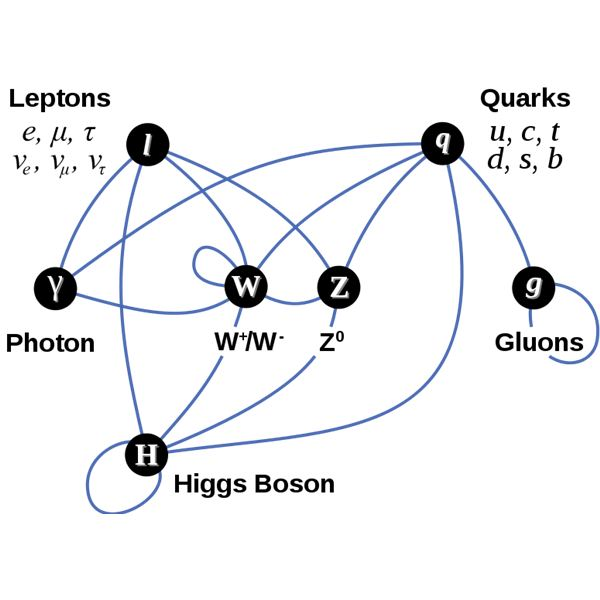
\includegraphics[width = 0.6\textwidth]{Pictures/elementaryParticles.jpg}
    %  \end{center}
    %  \end{block}
    %  
    %  \vspace{-0.25cm}
    %  \uncover<5->{
    %    \begin{block}{Antimatter:}
    %      \begin{itemize}
    %        \item To each fermion is associated an anti-fermion
    %        \item Same quantum numbers as fermions BUT opposite electric charge
    %      \end{itemize}
    %    \end{block}
    %  }

    %  \vspace{-0.25cm}
    %  \uncover<6->{\begin{block}{Forces:}
    %  \begin{center}
    %    \begin{tabular}{c c c c}
    %    \multirow{5}*{\uncover<6->{Bosons}} & \uncover<7->{$\gamma$} & \uncover<7->{$\rightarrow$} & \uncover<7->{E.M. interaction} \tabularnewline
    %    & \uncover<8->{$Z^{0}/W^{\pm}$} & \uncover<8->{$\rightarrow$} & \uncover<8->{Weak interaction} \tabularnewline
    %    & \uncover<9->{$g$ & $\rightarrow$} & \uncover<9->{Strong interaction} \tabularnewline
    %    & \uncover<10->{\textcolor{gray}{graviton} & \textcolor{gray}{$\rightarrow$}} & \uncover<10->{\textcolor{gray}{Gravitation}} \tabularnewline
    %    %\only<11->{\hline}
    %    & \uncover<11->{$H$ & $\rightarrow$} & \uncover<11->{Higgs field} \tabularnewline
    %    \end{tabular}
    %  \end{center}
    %  \end{block}}

    %\end{frame}

   \begin{frame}
     \frametitle{Standard Model}

     %\begin{block}{Standard Model:}
        \begin{itemize}
          \item Well-tested physics theory: predicts precisely a wide variety of phenomena with elementary particles
          \item Predicts a mechanism which breaks the electroweak symmetry (EWSB) and generates mass of particles \\
          $\Rightarrow$ Higgs mechanism: one gauge boson is expected in the SM (the Higgs boson)
          %\item Mass generation mechanism of particles: Higgs mechanism and electroweak symmetry breaking (EWSB)
          %\item Electro-Weak Symmetry Breaking (EWSB): explain how particles acquire mass via Higgs mechanism
          \item Last milestone: discovery of a particle compatible with the Higgs Boson, which would confirm the EWSB
        \end{itemize}
      
      \begin{center}
        $\Rightarrow$ Complete spectrum of Standard Model that could be correct up to very high energies
      \end{center}
     %\end{block}

   \end{frame} 
    
    \begin{frame}
      \frametitle{Open questions}

      %\begin{block}{Standard model:}
      %  \begin{itemize}
      %    \item Well-tested physics theory: predict precisely a wide variety of phenomena
      %    \item Electro-Weak Symmetry Breaking (EWSB): explain how particles acquire mass via Higgs mechanism
      %    \item Last milestone: discovery of the Higgs Boson
      %    %\item EWSB: explain how particle acquires mass
      %  \end{itemize}
      %\end{block}

      \begin{alertblock}{Limitations}
        \begin{itemize}
          \item Why electroweak symmetry is broken?
          \item Is there only one Higgs boson as defined in SM?
          \item Why are they 3 generations of leptons and quarks?
          \item Neutrino oscillation (theory does not predict mass of neutrino)
          \item What are the dark matter and the dark energy?
        \end{itemize}
      \end{alertblock}
          %\centering{\textbf{$\Rightarrow$ Need new experimental program}} 
      
    \end{frame}
    
    \begin{frame}
    \frametitle{How to study particle physics?}

    \only<1>{
      \vspace{0.3cm}
      \centering
      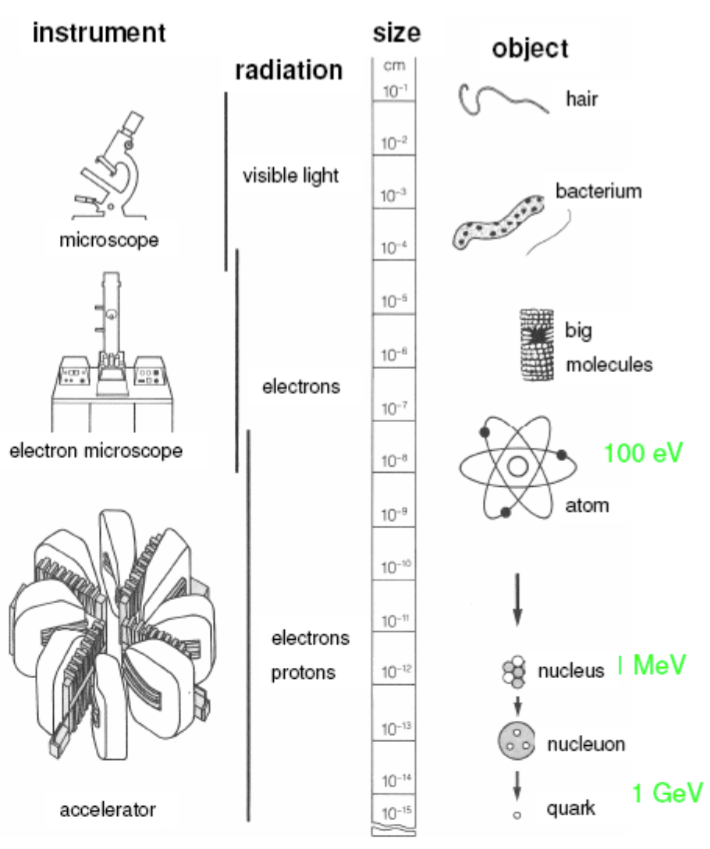
\includegraphics[width = 5cm]{Pictures/instrument.png}
    }

    \uncover<2->{
      \begin{columns}[c]
        \begin{column}{4cm}
          \centering
          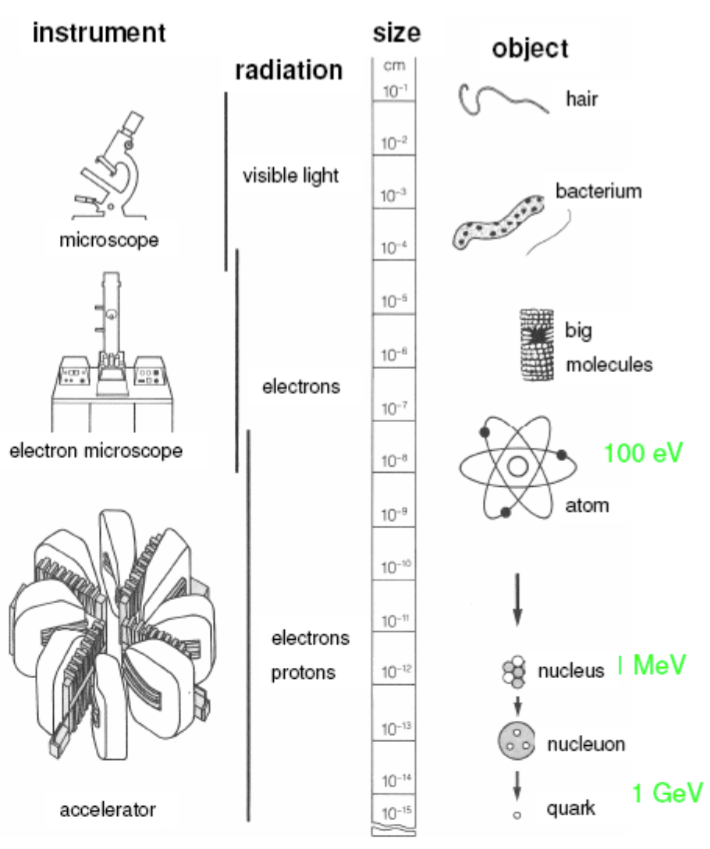
\includegraphics[width = 5cm]{Pictures/instrument.png}
        \end{column}
        \begin{column}{5cm}
          \centering
          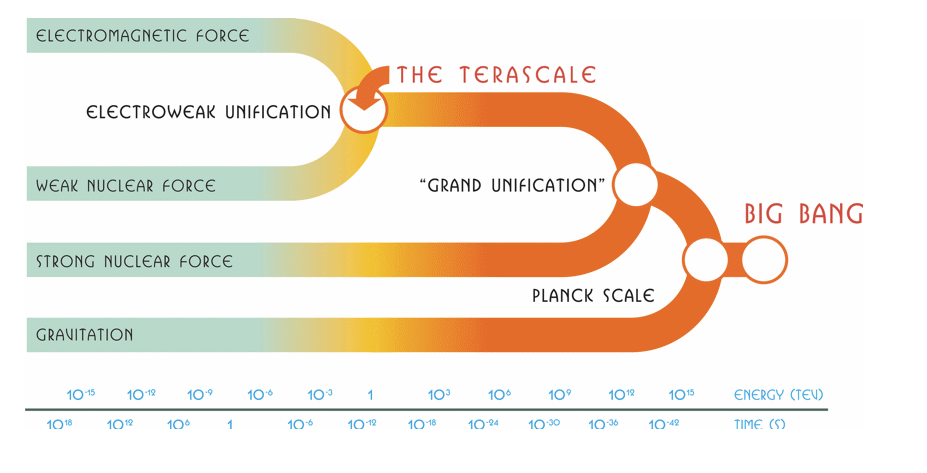
\includegraphics[width = 6cm]{Pictures/terascale_schematic.png}
          \
          EWSB and physics beyond SM: from 100 GeV to TeV scale
        \end{column}
      \end{columns}  
    }

    \uncover<3>{
      \vspace{0.1cm}
      \centering
      What tools do we have to reach this energy scale?
    }

    %\vspace{-0.15cm}
    %\begin{columns}[c]
    %  \begin{column}{5cm}
    %    \centering
    %    \uncover<2->{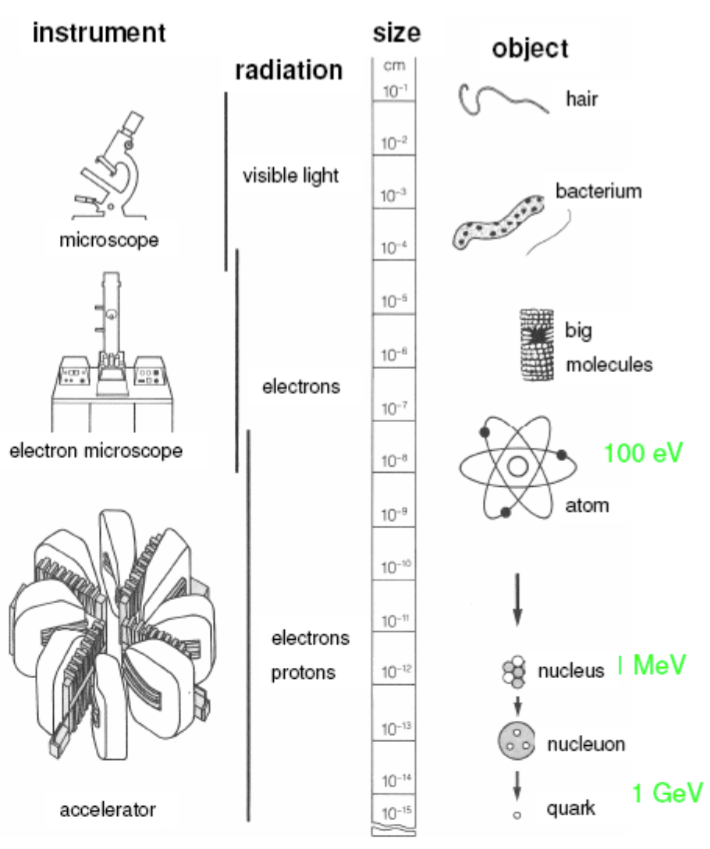
\includegraphics[width = 5cm]{Pictures/instrument.png}
    %    \footnotesize{
    %    EWSB and physics beyond SM: from 100 GeV to TeV scale
    %    }}
    %    
    %  \end{column}
    %  
    %  \begin{column}{5cm}
    %    \uncover<3->{\begin{block}{LHC: a discovery machine}
    %      \begin{itemize}
    %        \item Centre-of-mass energy $\sqrt{s} = 14~\text{TeV}$
    %        \item Collision with composites particles (protons or Pb)
    %            \begin{itemize}
    %                \item Unknown momentum distribution of partons
    %                \item Unknown polarisation of colliding partons
    %                \item Trigger needed
    %                \item Background made of complex Standard Model reactions
    %            \end{itemize}
    %      \end{itemize}
    %    \end{block}
    %    }
    %  \end{column}
    %\end{columns}

    %\vspace{0.1cm}
    %\uncover<3>{\centering{\textbf{$\Rightarrow$ Need complementary experimental program}} }
  \end{frame}

  \begin{frame}
    \frametitle{Large Hadron Collider (LHC)}

    \uncover<1->{
    \begin{columns}[c]
      \begin{column}{4cm}
        \centering

        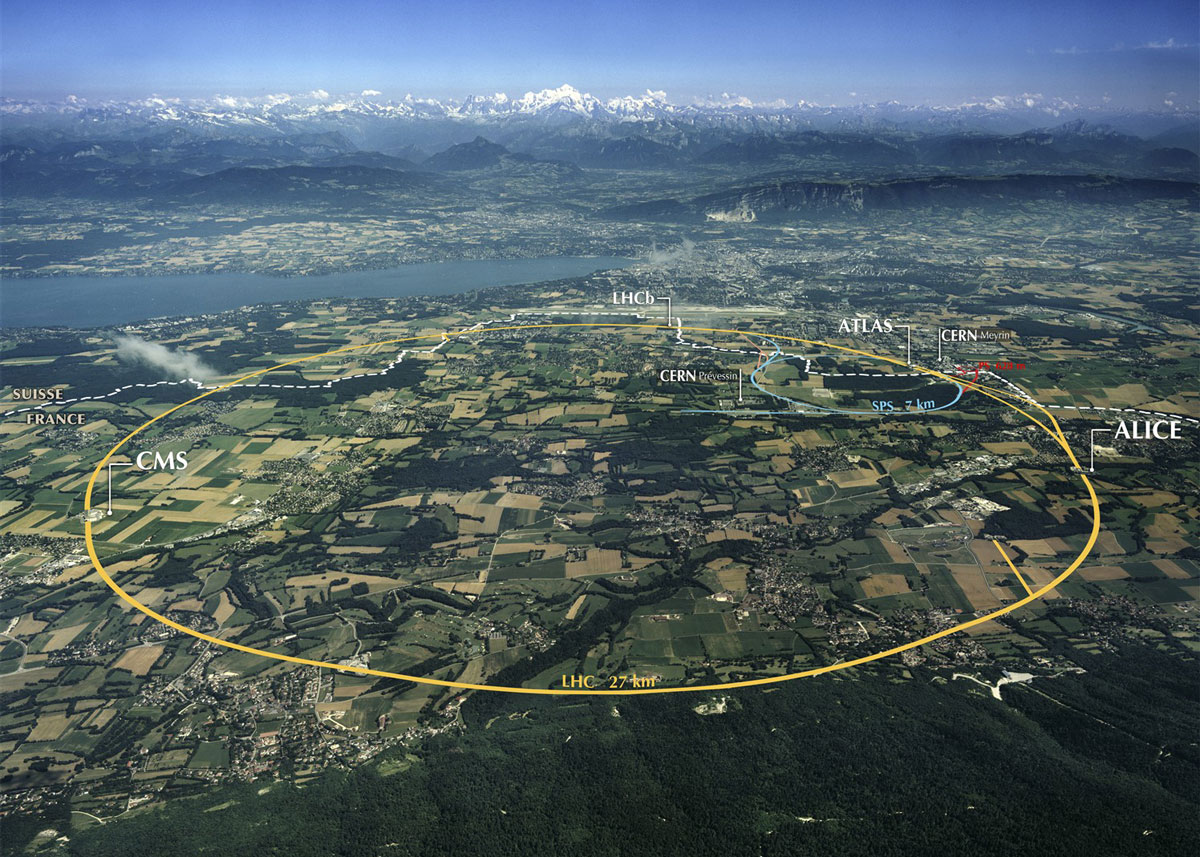
\includegraphics[width =\textwidth]{Pictures/cern-lhc-aerial.jpg}
      \end{column}

      \begin{column}{6cm}
        \begin{block}{LHC: a discovery machine}
          \begin{itemize}
            \item Centre-of-mass energy $\sqrt{s} = 14~\text{TeV}$
            \item Collision with composites particles (protons or Pb)
                \begin{itemize}
                    \item Unknown momentum distribution of partons
                    \item Unknown polarisation of colliding partons
                    \item Trigger needed
                    \item Background made of complex Standard Model reactions
                \end{itemize}
          \end{itemize}
        \end{block}
      \end{column}
    \end{columns}
    }

    \uncover<2>{
      \vspace{0.3cm}
      \centering{\textbf{$\Rightarrow$ Need complementary experimental program}}
    }

  \end{frame}

    
    \subsection{ILC and ILD}
%-------------------------------
%   Intro: ILC 
%-------------------------------

  \begin{frame}
    \frametitle{International Linear Collider}

    \vspace{-0.3cm}
    \begin{columns}[c]
      \begin{column}{3cm}
        \centering
        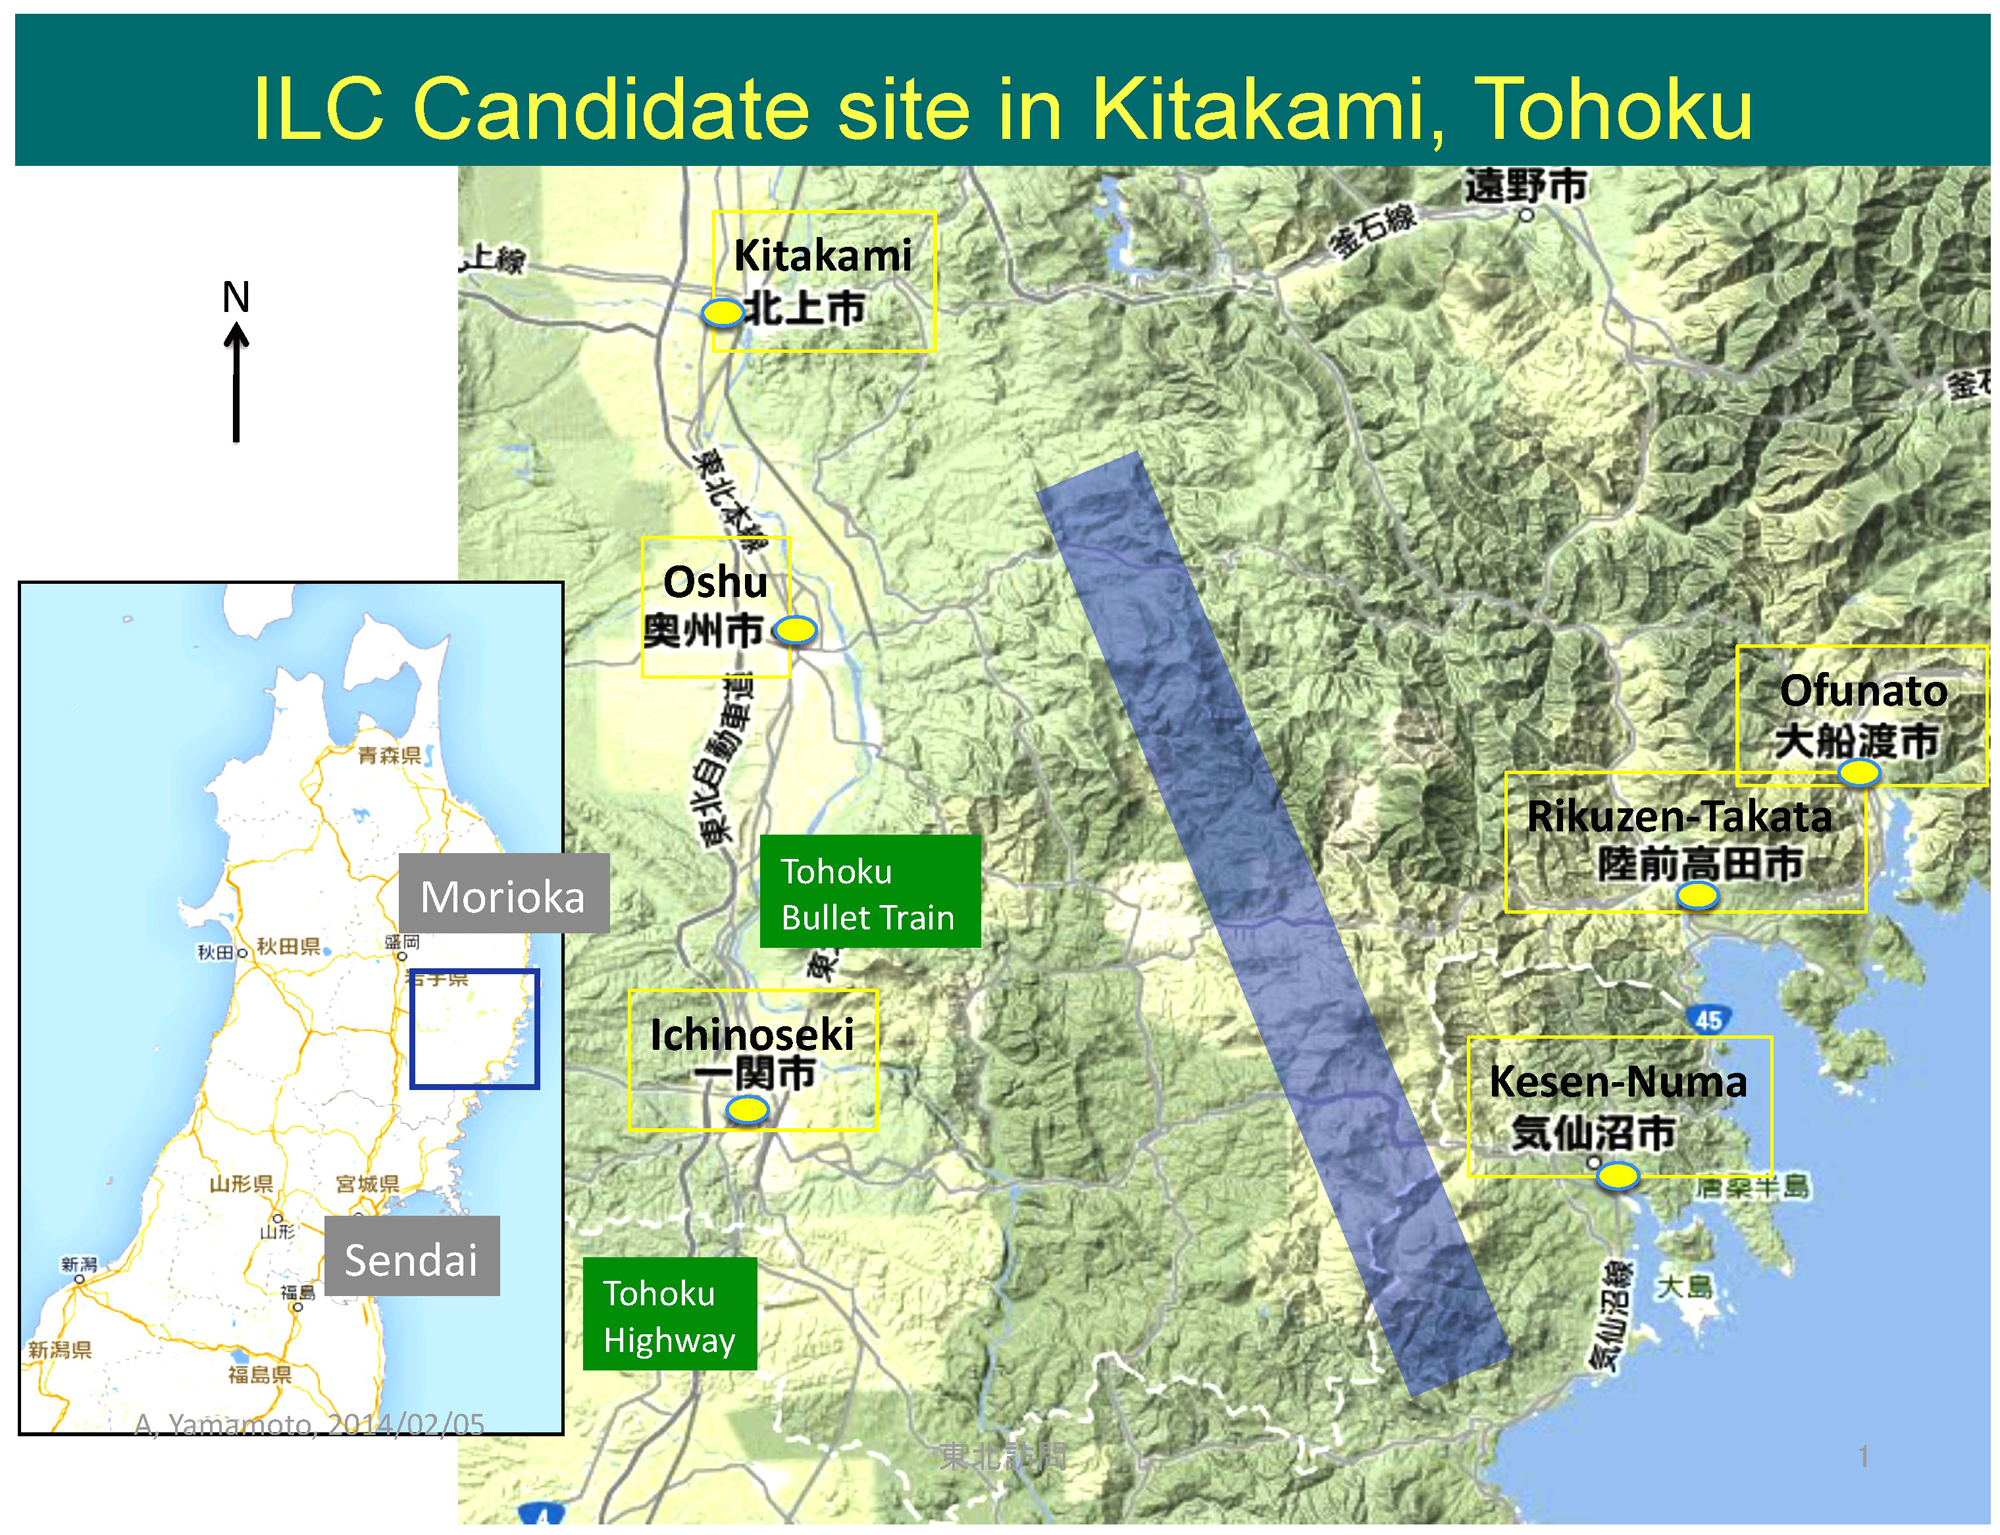
\includegraphics[width = 4 cm]{Pictures/ILC-Candidate-Area2.jpg}
      \end{column}
      \begin{column}{8cm}
        \centering
        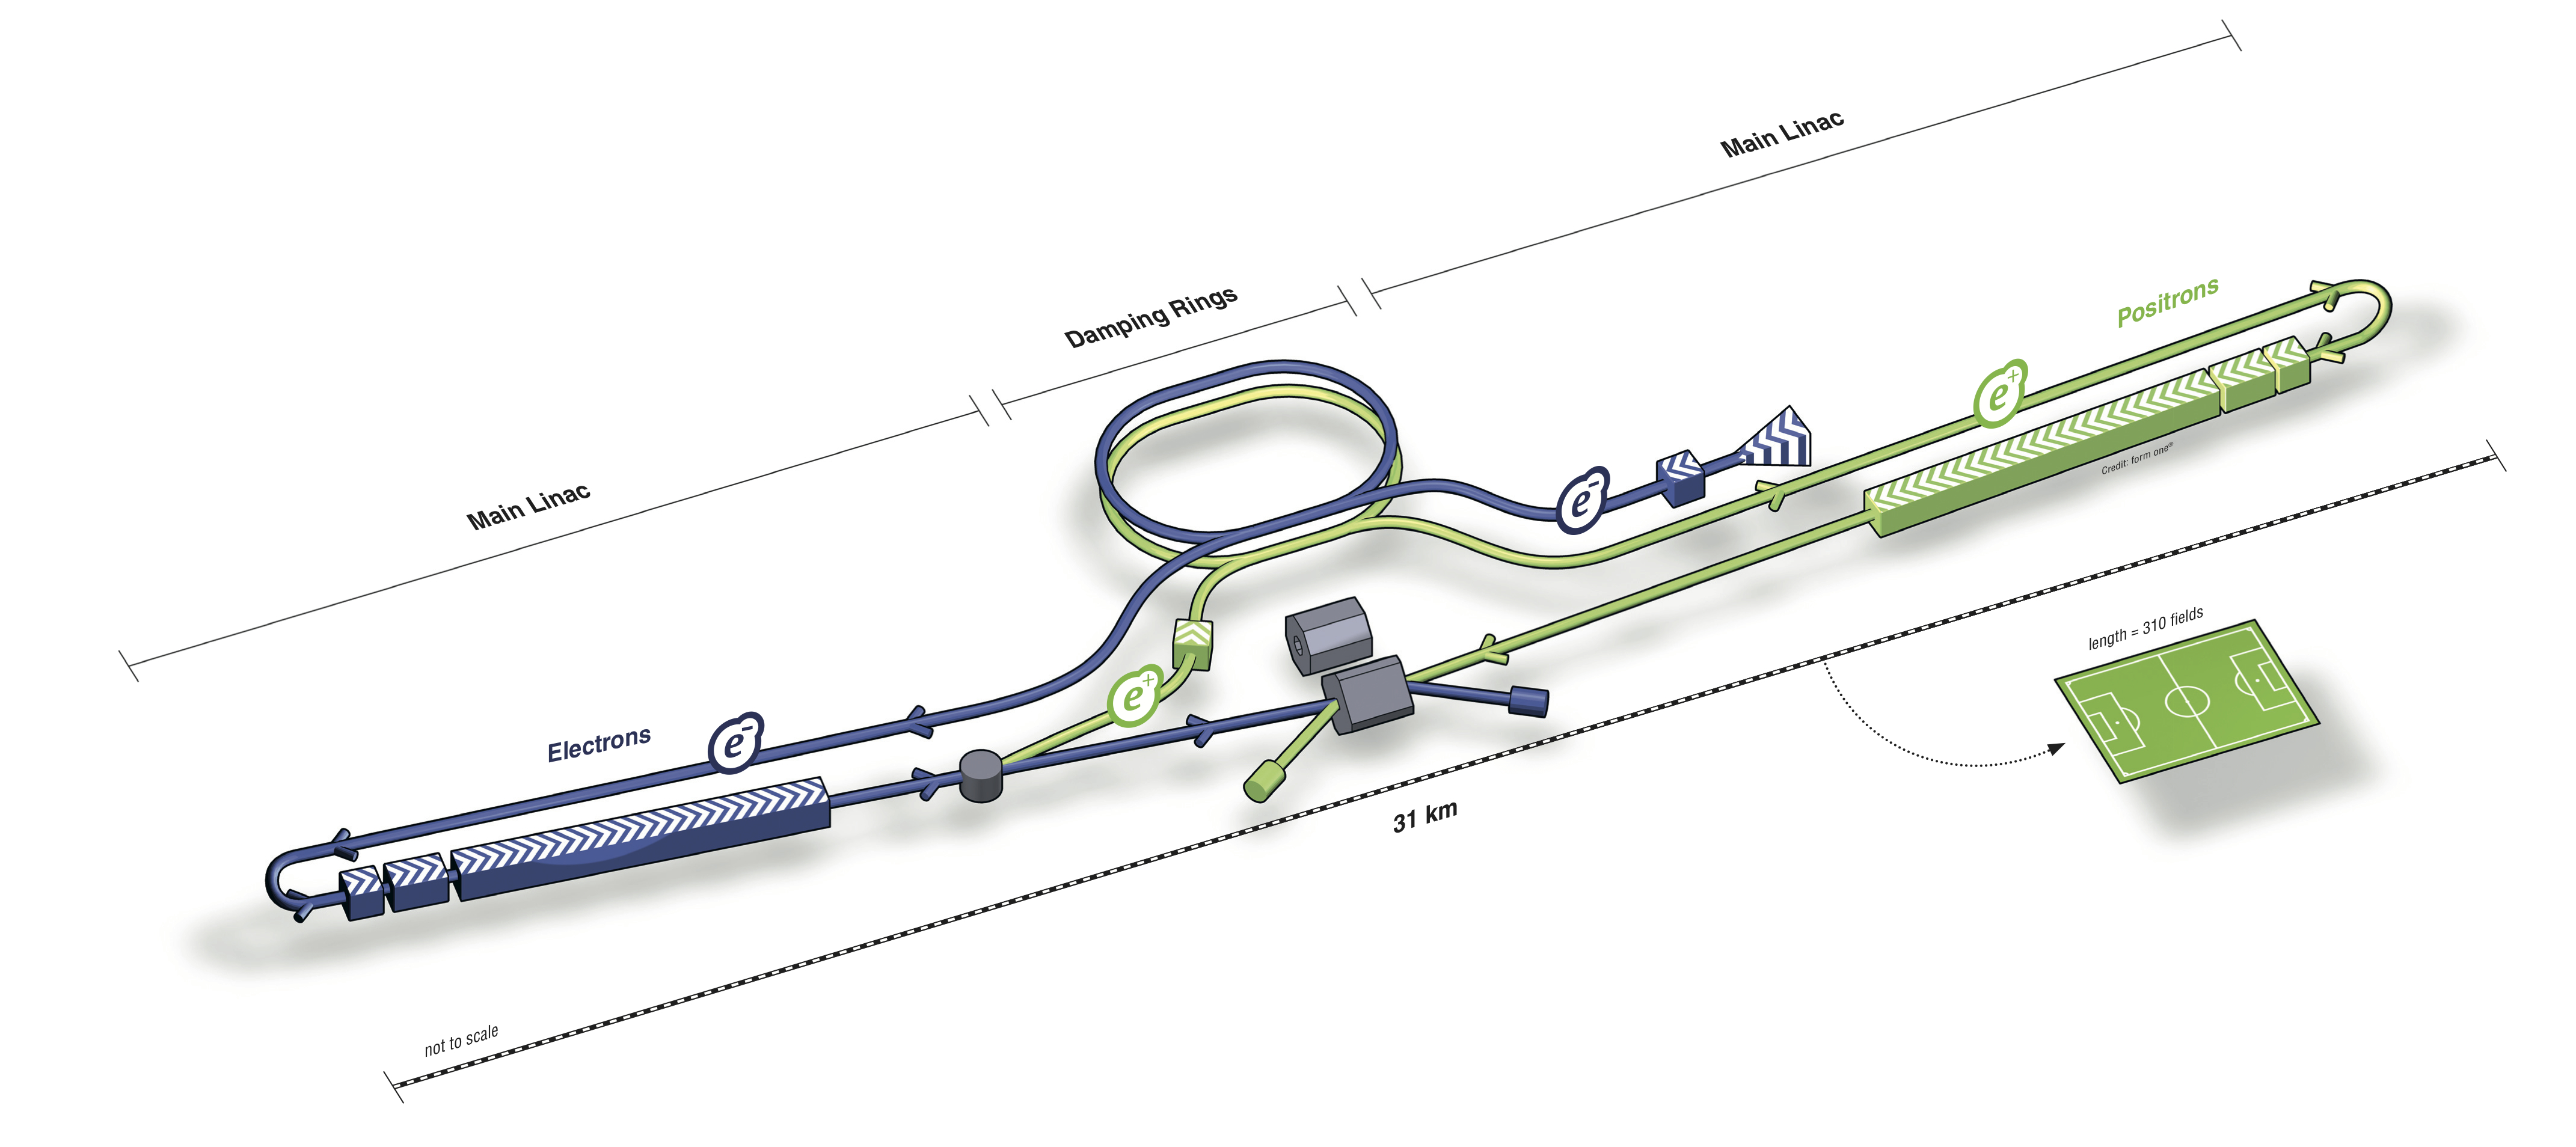
\includegraphics[width = 9 cm]{Pictures/ILC.png}
      \end{column}
    \end{columns}

    \vspace{-0.3cm}
    \begin{itemize}
      \item Future $\rm{e}^+\rm{e}^-$ linear collider at $\sqrt{s} = 250 - 500~\rm{GeV}$ \\ (upgrade up to $\sqrt{s} = 1~\rm{TeV}$)
      \item Polarised beam
      \item Luminosity $\simeq 2 \times 10^{34}~\rm{cm}^{-2}\rm{s}^{-1}$
      \item Candidate site: Kitakami in nothern Japan
      \item To study properties of the Higgs boson, top physics and discovery potential new physics
    \end{itemize}
  \end{frame}
 
 %-------------------------------
%                           Intro: ILD VS SiD 
%-------------------------------

\begin{frame}
  \frametitle{SiD and ILD}

  \begin{columns}[t]
    \begin{column}{5cm}
      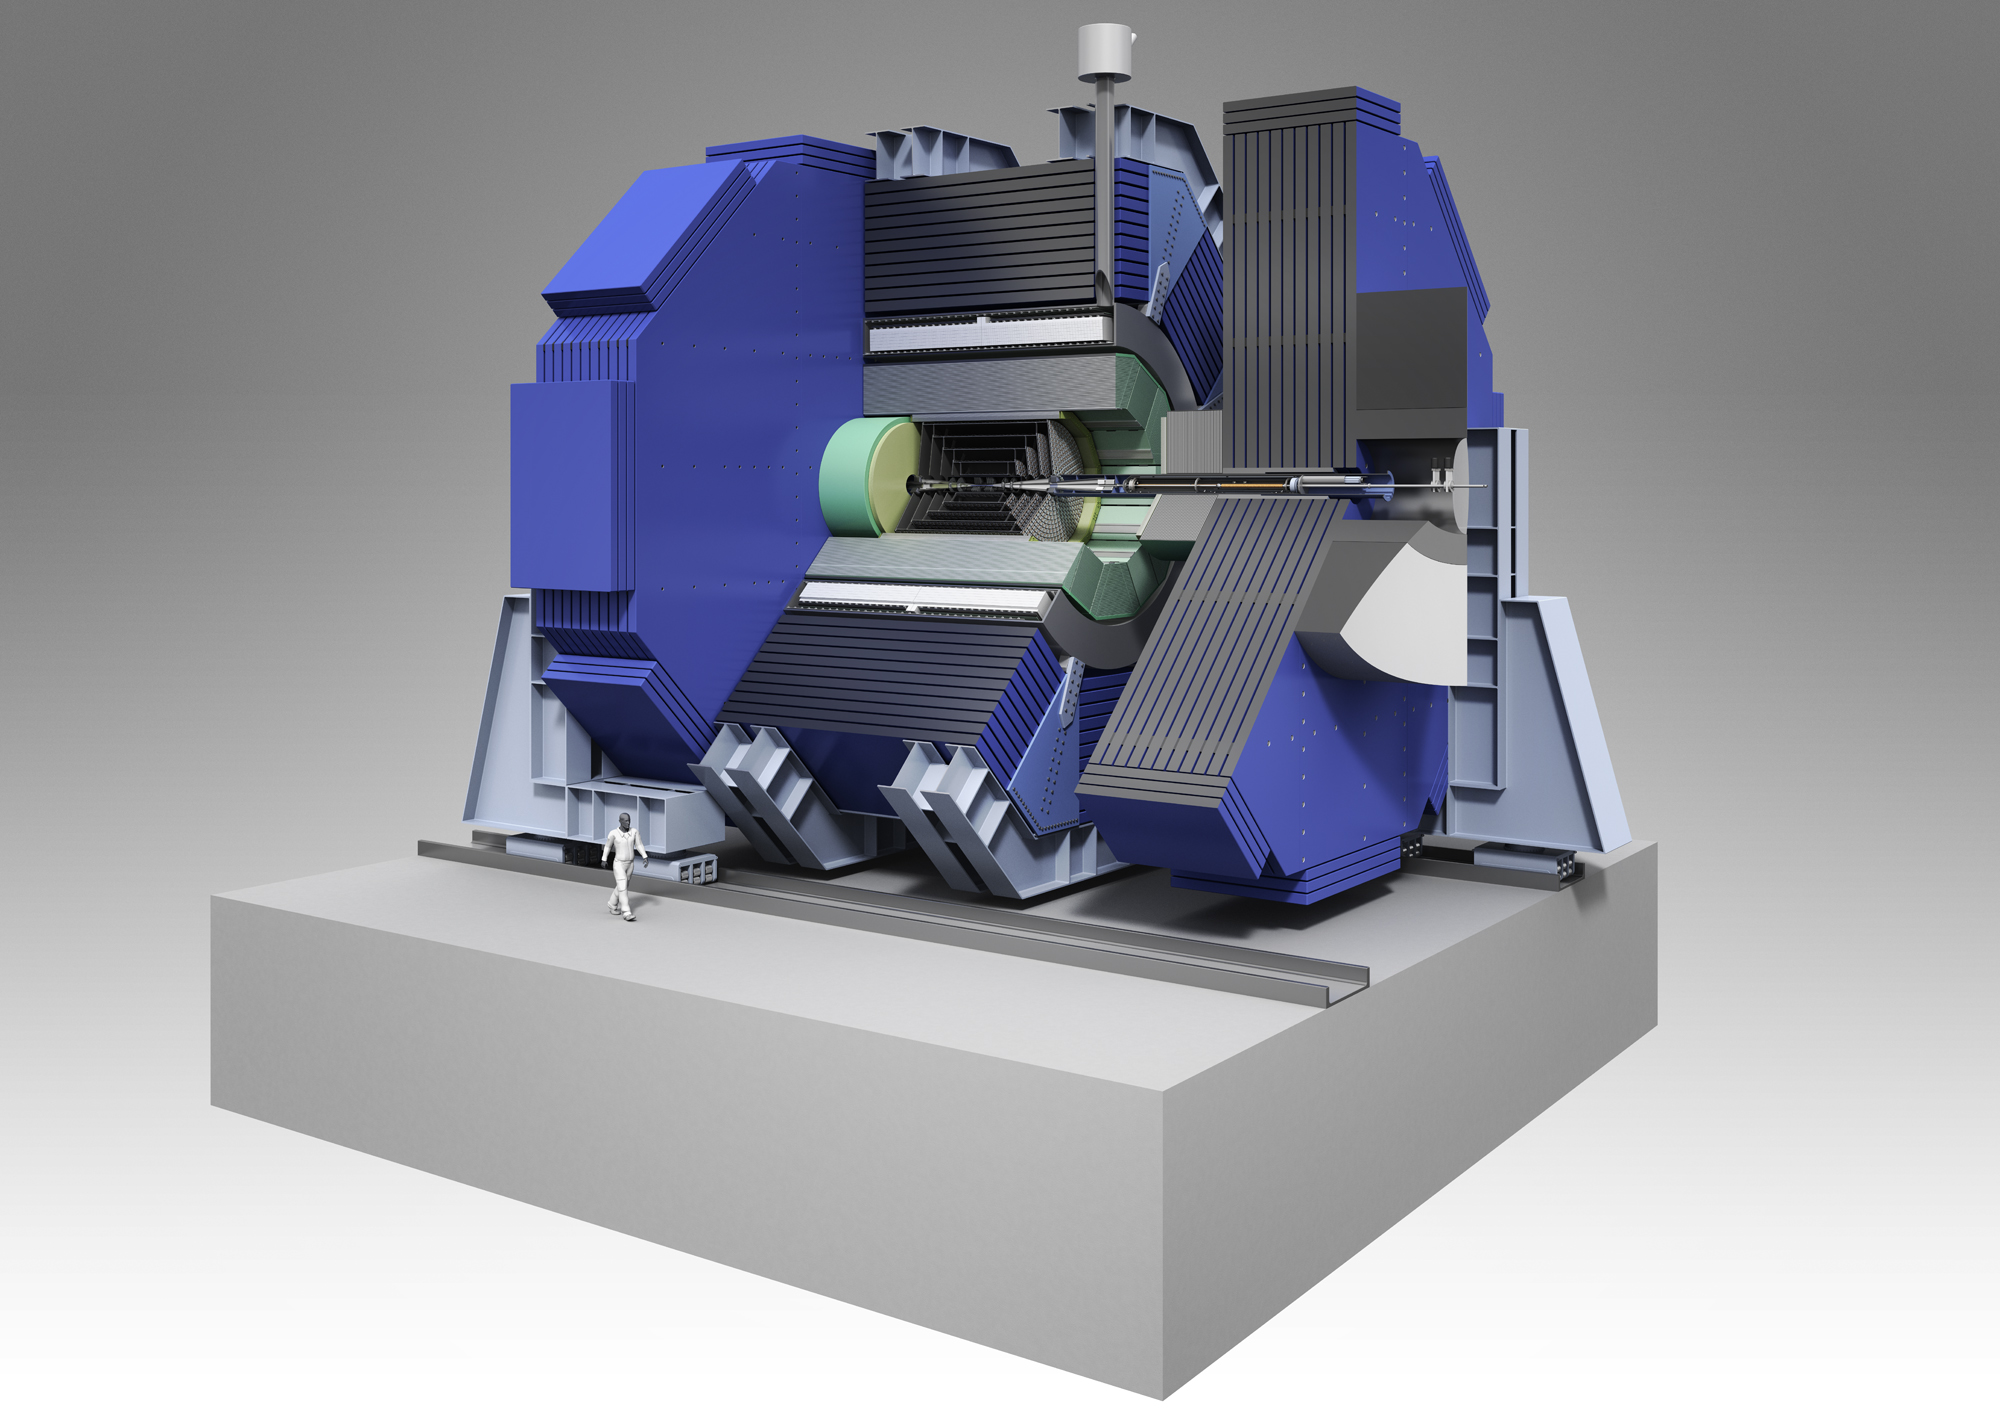
\includegraphics[width = 5cm, height = 2.9 cm]{Pictures/ILC_SiD.jpg}
      \vspace{-0.25cm}
      \begin{block}{Silicon Detector}
        \footnotesize{
        \begin{itemize}
          \item Silicon tracking \\ (radius = 1.2 m)
          \item B$_{field}$ = 5 T
        \end{itemize}
        }
      \end{block}
    \end{column}

    \begin{column}{5cm}
      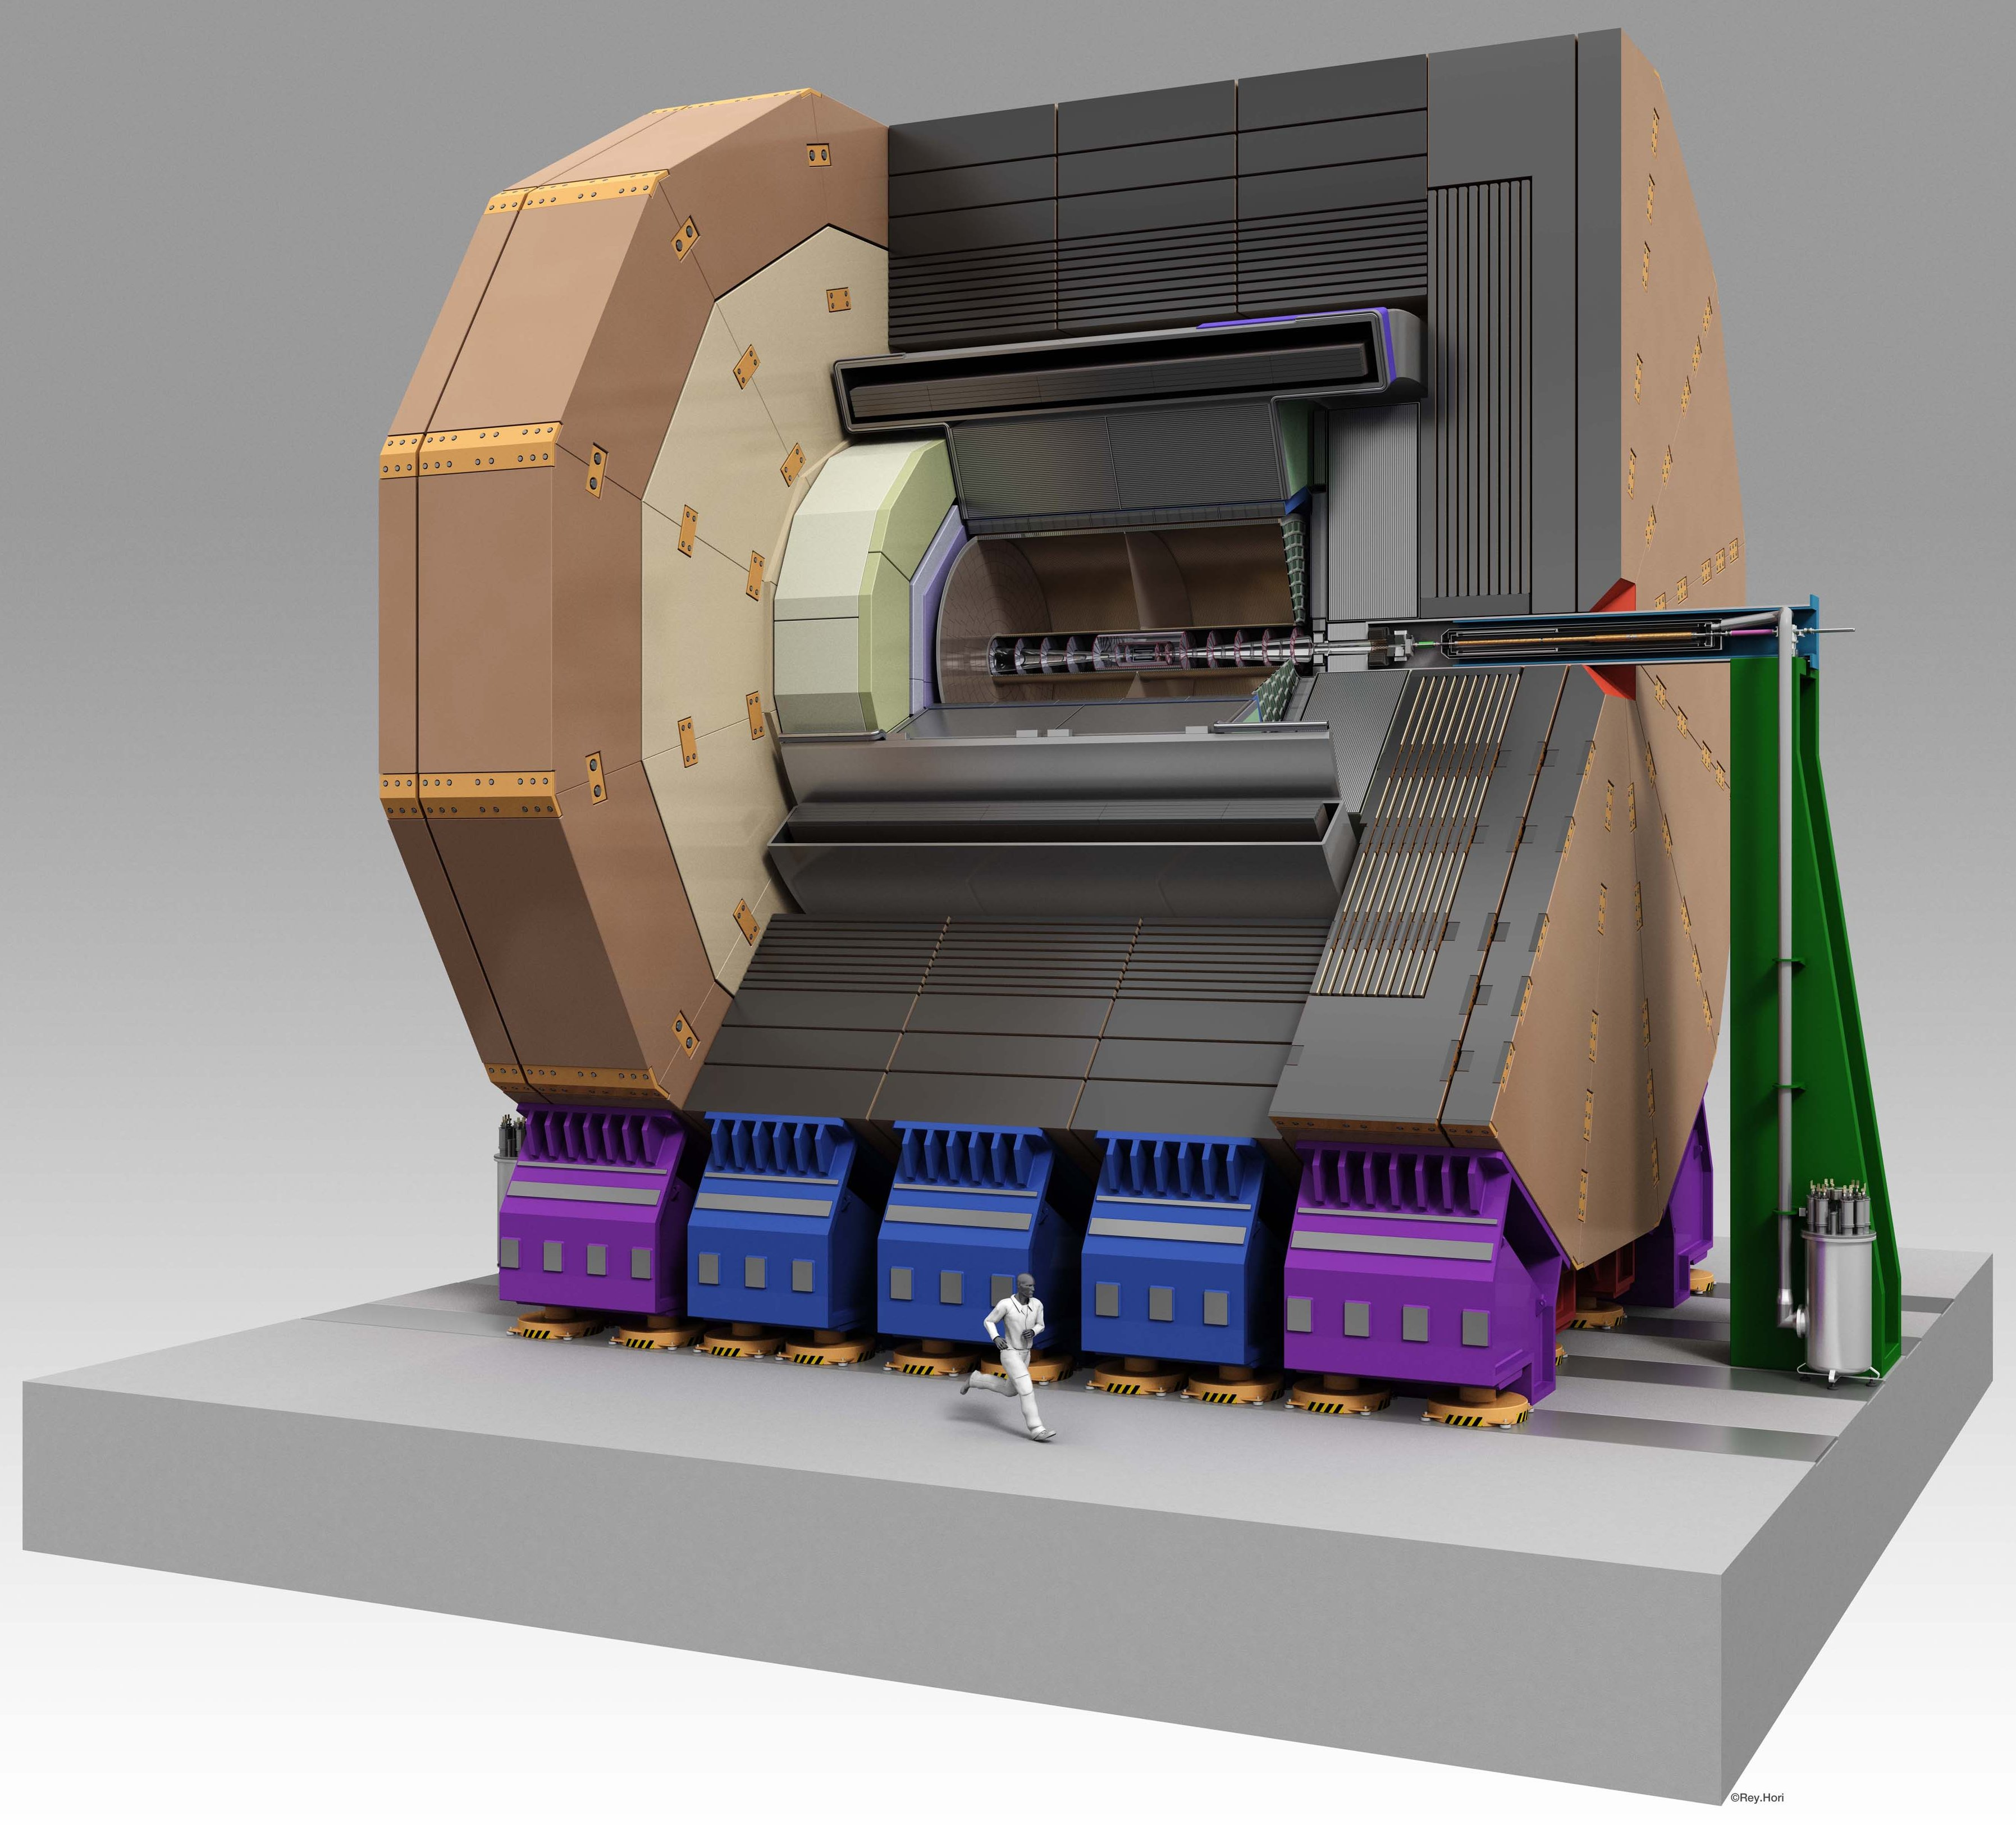
\includegraphics[width = 5cm, height = 2.9 cm]{Pictures/ILD_all_110826.jpg}
      \vspace{-0.25cm}
      \begin{block}{International Large Detector}
        \footnotesize{
        \begin{itemize}
          \item TPC + silicon envelope \\ (radius = 1.8 m)
          \item B$_{field}$ = 3.5 T
        \end{itemize}
        }
      \end{block}
    \end{column}
  \end{columns}

  \begin{block}{Both detectors designed for Particle Flow Calorimetry}
    \footnotesize{
    \begin{itemize}
      \item High granularity calorimeters (ECAL and HCAL) inside solenoid
      \item Low mass tracker to reduce interactions and conversions
    \end{itemize}
    }
  \end{block}
  
\end{frame}

\begin{frame}
  \frametitle{Particle Flow Algorithm}

  \begin{center}
    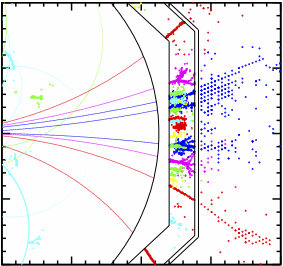
\includegraphics[width = 0.5\textwidth]{Pictures/ild_particleFlowConcept.png}
  \end{center}
\end{frame}
  
\section{Higgs boson study at the ILC}
  \begin{frame}
    \frametitle{Outlines}
    \begin{minipage}{\textwidth}
      \tableofcontents[currentsection,hideothersubsections, 
      sectionstyle=show/shaded,]
    \end{minipage}
  \end{frame}

  \subsection{Motivation}

    \begin{frame}
      \frametitle{Higgs boson study}

      \vspace{-0.3cm}
      \begin{block}{Measurements @ LHC}
        \begin{itemize}
          \item Higgs boson discovered in 2012 (ATLAS and CMS collaborations)
          \item Mass: $125.7 \pm 0.4$ GeV
          \item Spin: 0
          %\item Only a subset of Higgs couplings can be observed (with uncertainties of $5~\%$)
        \end{itemize}
      \end{block}
          
      \vspace{-0.1cm}
      \begin{columns}[c] 

        \begin{column}{5cm}
          \centering
          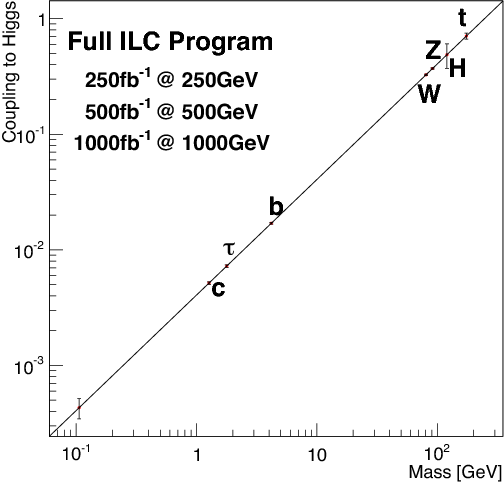
\includegraphics[width = 4cm]{Pictures/Chapter_Theory_figs_mass-coupling1TeV.png}
        \end{column}
        \begin{column}{5cm}
          \centering
          \begin{alertblock}{Missing measurements}
            \begin{itemize}
              \item Couplings of Higgs boson to $c$-quarks and gluons
              \item Higgs self-coupling 
            \end{itemize}
            \centering
            $\Rightarrow$ Is the boson discover compatible with the Higgs boson defined in the SM?
          \end{alertblock}
        \end{column}

      \end{columns}

    \end{frame}

    \begin{frame}
    \frametitle{Higgs boson study at the ILC}

    \vspace{-0.3cm}
    \begin{columns}[c]
      \begin{column}{5cm}
        \begin{center}
          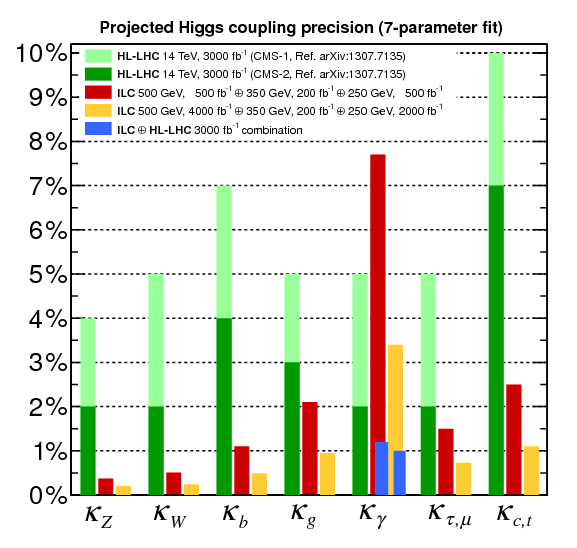
\includegraphics[width = 5cm]{Pictures/Figures_HiggsCoupling500LHC.png}
          %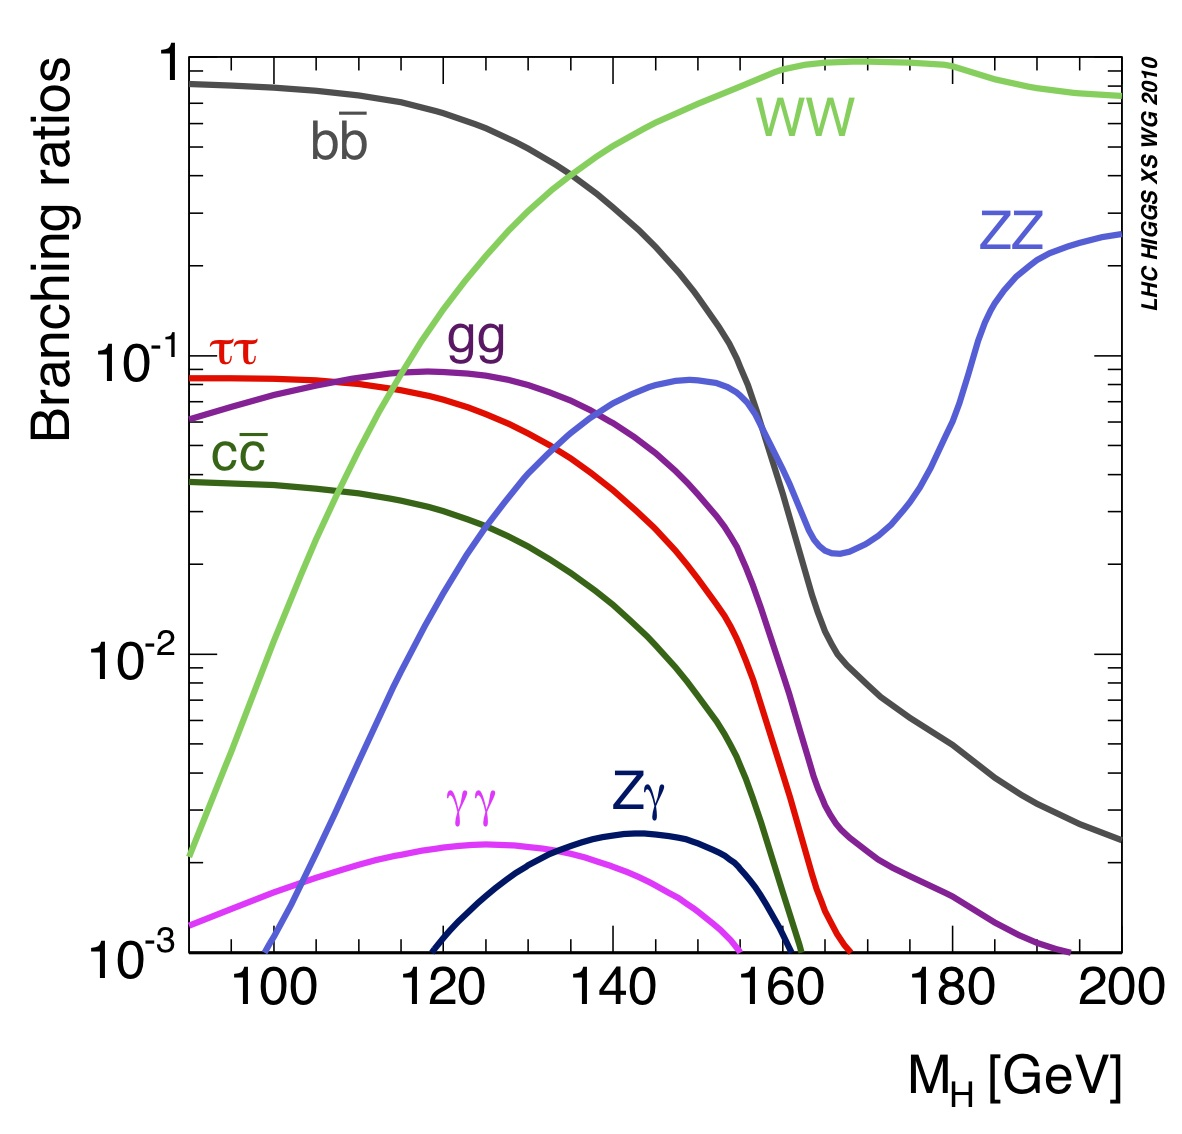
\includegraphics[width = 5cm]{Pictures/higgsbr.jpg}
        \end{center}
      \end{column}
      \begin{column}{5cm}
        \begin{block}{At the LHC}
          \footnotesize
          \begin{itemize}
            \item Higgs boson to quarks difficult to observe
            \item $H \rightarrow b\overline{b}$ observed in special kinematics
            \item $H \rightarrow c\overline{c}$ and $H \rightarrow gg$ are challenging to observe
          \end{itemize}
        \end{block}
        \vspace{-0.3cm}
        \begin{block}{At the ILC}
          \footnotesize
          \begin{itemize}
            \item $H \rightarrow b\overline{b}, c\overline{c}, WW^{*}, \tau\tau$ and $gg$ able to be separately identified with high efficiency 
          \end{itemize}
        \end{block}

      \end{column}
    \end{columns}

    \vspace{-0.1cm}
    \begin{center}
      Analysis of simulated data at the ILC @ \hyperlink{Xsec}{350 GeV} with different polarisations:
        \vspace{-0.2cm}
        \begin{itemize}
          \item $e^+_L e^-_R$
          \item $e^+_R e^-_L$
        \end{itemize}
    \end{center}

\end{frame}

  \subsection{Study of the H$\nu\nu$ final state}
\begin{frame}
  %\frametitle{How to perform the analysis?}
  \frametitle{Study of H$\nu\nu$ final state}

  \tikzset{
    particle/.style={thick,draw=black, postaction={decorate},
    decoration={markings,mark=at position .5 with {\arrow[black]{triangle 45}}}},
    aparticle/.style={thick,draw=black, postaction={decorate},
    decoration={markings,mark=at position .5 with {\arrow[black]{triangle 45 reversed}}}},
    gluon/.style={decorate, draw=black,
    decoration={coil,aspect=0}}
  }

  \vspace{-0.3cm}
  \begin{itemize}
    \item Study final state leading to H$\nu\nu$ channel where the Higgs boson decays into a pair of quarks or gluons
    \item Focus on Higgs Strahlung and WW fusion:
  \end{itemize}
  \vspace{-0.3cm}
  \begin{center}
    $m_H~\simeq~125~\text{GeV and }\sqrt{s} = 350~\text{GeV} \Rightarrow$ Higgs Strahlung and WW-fusion have comparable \hyperlink{Xsec}{cross sections}.  
  \end{center}
  \vspace{-0.1cm}
  \begin{columns}[c]
    \begin{column}{5cm}
      %\includegraphics[width = 6cm]{../../Crap/Pictures/higgsstrahlung.jpg}
      \begin{tikzpicture}[node distance=1cm and 1.5cm]
        \coordinate[label=left:$e^{+}$] (p1);
        \coordinate[below right=of p1] (aux1);
        \coordinate[below left=of aux1, label=left:$e^{-}$] (e1);
        \coordinate[right=1.25cm of aux1] (aux2);
        \coordinate[above right=of aux2,label=right:$H$] (higgs);
        \coordinate[below right=1cm of aux2, label=left:$Z$] (Z);
        \coordinate[above right=1cm of Z, label=right:$\nu$] (nu);
        \coordinate[below right=1cm of Z, label=right:$\overline{\nu}$] (nuB);

        \draw[aparticle] (p1) -- (aux1);
        \draw[aparticle] (aux1) -- (e1);
        \draw[dashed,red] (higgs) -- (aux2);
        \draw[gluon] (aux2) -- (Z);
        \draw[gluon] (aux1) -- node[label=above:$Z^*$] {} (aux2);
        \draw[particle] (Z) -- (nu);
        \draw[aparticle] (Z) -- (nuB);
      \end{tikzpicture}
    \end{column}

    \begin{column}{5cm}
      \begin{tikzpicture}[node distance = 1cm and 1.2cm]
        \coordinate[label=left:$e^{+}$] (p1);
        \coordinate[below right=of p1] (aux1);
        \coordinate[above right=of aux1,label=right:$\overline{\nu}$] (nuB);
        \coordinate[below=0.85cm of aux1,xshift=0.5cm] (aux2);
        \coordinate[right=of aux2, label=right:$H$] (higgs);
        \coordinate[below=0.85cm of aux2,xshift=-0.5cm] (aux3);
        \coordinate[below left=of aux3,label=left:$e^{-}$] (e1);
        \coordinate[below right=of aux3,label=right:$\nu$] (nu);

        \draw[aparticle] (p1) -- (aux1);
        \draw[aparticle] (aux1) -- (nuB);
        \draw[dashed,red] (aux2) -- (higgs);
        \draw[gluon] (aux1) -- node[label=left:$W$] {} (aux2);
        \draw[gluon] (aux2) -- node[label=left:$W$] {} (aux3);
        \draw[particle] (e1) -- (aux3);
        \draw[particle] (aux3) -- (nu);
      \end{tikzpicture}
      %\includegraphics[width = 6cm]{../../Crap/Pictures/HiggsProd_vvH.png}
    \end{column}
  \end{columns}

  \vspace{-0.3cm}
  \begin{center}
    Using polarised beam to separate the processes.
  \end{center}
\end{frame}

%-------------------------------
%                           How to
%-------------------------------

\begin{frame}
  \frametitle{Reconstruction of the H$\nu\nu$ channel}

  \begin{block}{Final state signature}
    \begin{itemize}
      \item 2 jets coming from the Higgs boson decay
      \item Missing energy
    \end{itemize}
  \end{block}

  \begin{block}{Events selection}
    \begin{enumerate}
      \item Reject events with isolated leptons
      \item Remove $\gamma\gamma$ overlay interactions 
      \item Look for jets
      \item Find displaced vertices of the jets
      \item Tag 2 jets coming from Higgs boson decay
    \end{enumerate}
  \end{block}
\end{frame}

\begin{frame}
  \frametitle{Background processes}

  %\begin{itemize}
  %\item
  {\footnotesize{
    \vspace{-0.3cm}
    \begin{block}{Events which give same detector response or same final state}
      \begin{itemize}
        \item W-boson pair production
          \vspace{-0.1cm}
          \begin{itemize}
            \item Semi-leptonic decay: $e^+e^- \ \rightarrow \ W^+W^- \ \rightarrow \  \nu_l l^{\pm}q\overline{q}$
            \item Hadronic decay: $e^+e^- \ \rightarrow \ W^+W^- \ \rightarrow \  q\overline{q}q\overline{q}$
          \end{itemize}
          \vspace{-0.2cm}
        \item Z-boson pair production
          \vspace{-0.1cm}
          \begin{itemize}
            \item $e^+e^- \ \rightarrow \  ZZ \rightarrow \ \nu_l \overline{\nu_l }q \overline{q}$ 
            \item $e^+e^- \ \rightarrow \  ZZ \rightarrow \ l^+ l^- q \overline{q}$ 
            \item $e^+e^- \ \rightarrow \  ZZ \rightarrow \ q \overline{q} q\overline{q}$ 
          \end{itemize}
          \vspace{-0.2cm}
        \item Single W-boson production
          \vspace{-0.1cm}
          \begin{itemize}
            \item $e^+e^- \ \rightarrow \ W^{\pm} e^{\pm} \nu_e \ \rightarrow \nu_ee^{\pm}q\overline{q}$
          \end{itemize}
          \vspace{-0.2cm}
        \item Single Z-boson production
          \vspace{-0.1cm}
          \begin{itemize}
            \item $e^+e^- \ \rightarrow \ Z e^-e^+ \ \rightarrow q\overline{q}e^-e^+$
            \item $e^+e^- \ \rightarrow \ Z \ q\overline{q} \ \rightarrow q\overline{q}q\overline{q}$
          \end{itemize}
          \vspace{-0.2cm}
        \item Higgsstrahlung:
          \vspace{-0.1cm}
          \begin{itemize}
            \item $e^+e^- \ \rightarrow ZH \ \rightarrow \ q\overline{q}q\overline{q}$ 
            \item $e^+e^- \ \rightarrow ZH \ \rightarrow \ l^+ l^- q \overline{q}$
          \end{itemize}
      \end{itemize}
    \end{block}
  }}
  %\end{itemize}
\end{frame}

\begin{frame}
  \frametitle{Distribution of the visible invariant mass with background}
  \begin{center}
    $\sqrt{s} = 350~\text{GeV}$, luminosity: $250~\text{fb}^{-1}$ and polarisation: e$^-_L$, e$^+_R$
    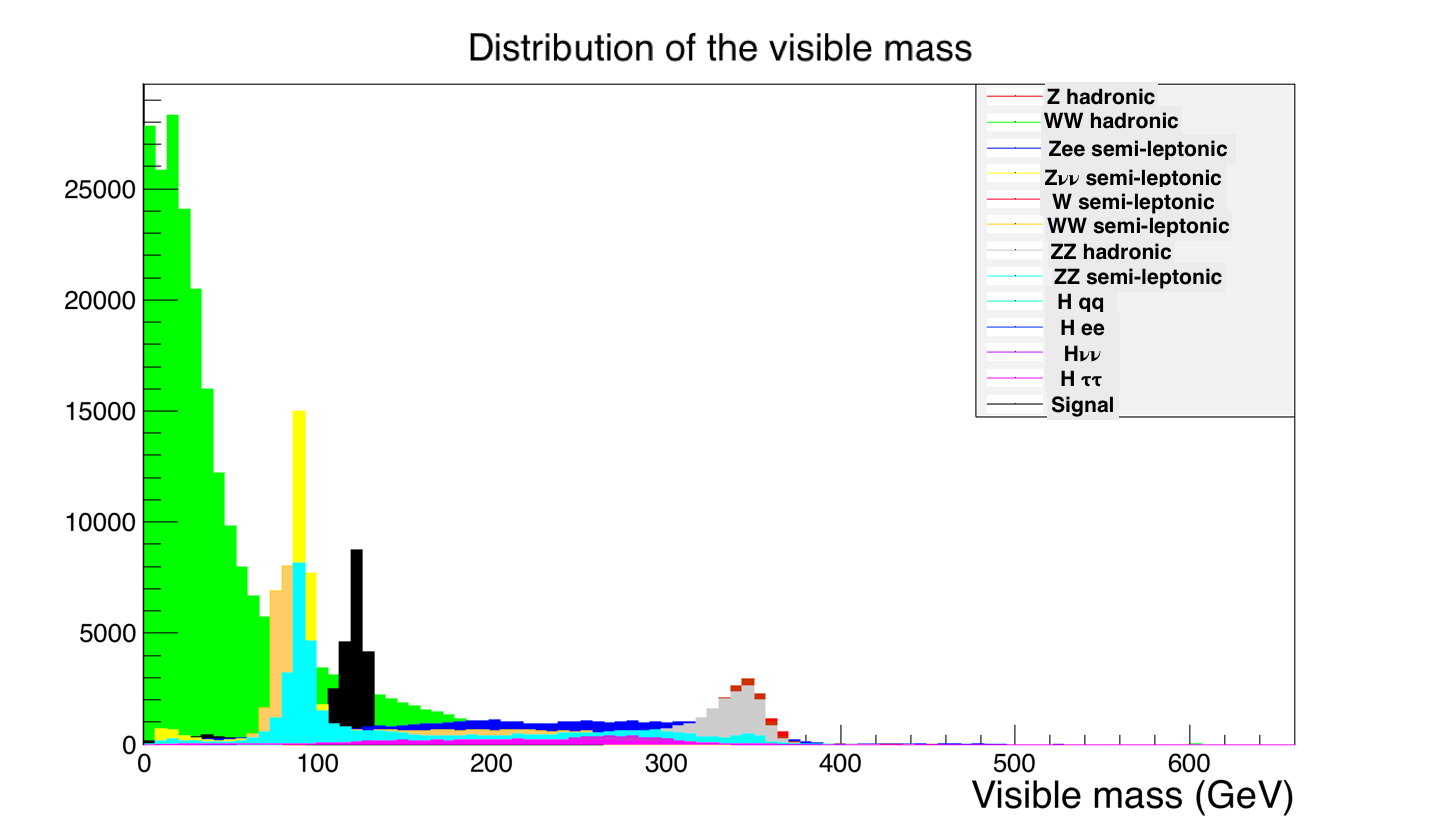
\includegraphics[width = \textwidth]{Pictures/mVis_all.png}
  \end{center}
  
  \begin{tikzpicture}[overlay,remember picture, red, shift={(current page.south west)}]
    \begin{scope}
      \draw[line width = 2pt,-latex] (6,4) -- (3.7,2.8);
    \end{scope}
  \end{tikzpicture}
  
  %\grille
\end{frame}

%\begin{frame}
%  \frametitle{Distribution of each processes}
%
%  \begin{center}
%    \footnotesize{
%      \begin{tabular}{c c}
%        \hline
%         Process        &  Expected events   \tabularnewline
%        \hline
%        \hline
%        $Z$ hadronic decay            & $1.3 \cdot 10^{7}$ \tabularnewline
%        $WW$ hadronic decay           & $2.2 \cdot 10^{6}$ \tabularnewline
%        $WW$ semi-leptonic decay      & $3.7 \cdot 10^{6}$ \tabularnewline
%        $ZZ$ hadronic decay           & $2.0 \cdot 10^{5}$ \tabularnewline
%        $ZZ$ semi-leptonic decay      & $1.9 \cdot 10^{5}$ \tabularnewline
%        $W$ semi-leptonic decay       & $5.4 \cdot 10^{5}$ \tabularnewline
%        $Zee$ semi-leptonic decay     & $1.0 \cdot 10^{5}$ \tabularnewline
%        $Z\nu\nu$ semi-leptonic decay & $1.2 \cdot 10^{5}$ \tabularnewline
%        Higgs BG                      & $5.3 \cdot 10^{4}$ \tabularnewline
%        Other Higgs boson decay       & $1.0 \cdot 10^{4}$ \tabularnewline
%        \hline
%        Background                    & $1.9 \cdot 10^{7}$ \tabularnewline
%        Signal                        & $2.2 \cdot 10^{4}$ \tabularnewline
%        \hline
%      \end{tabular}
%    }   
%  \end{center}
%\end{frame}

  \subsection{Reduction of the background}
\begin{frame}
  \frametitle{Reducing the background}
    
  \vspace{-0.25cm}
  \begin{block}{Find optimized cuts}
      \begin{itemize}
          \item For each cut, try to find the one which reduces the signal the least
              \[significance = \frac{signal}{\sqrt{signal + background}}\]
          \item Apply the cuts from the one which gives best significance to the one gives the worst
      \end{itemize}
  \end{block}

  \vspace{-0.2cm}
  \begin{exampleblock}{\hyperlink{cuts}{Sequential cuts strategy}}
      \begin{enumerate}
          \item [cut0] Number of isolated lepton (niso): niso = 0 %-1 < niso < 1
          \item [cut1] Transverse Momentum visible ($\rm{P_{t}^{vis}}$): 35 < $\rm{P_{t}^{vis}}$ < 155 GeV
          \item [cut2] Visible mass ($\rm{m_{vis}}$): 95 < $\rm{m_{vis}}$ < 140 GeV
          \item [cut3] Angle between the momentum axis of both jets ($\cos{\alpha}$):\\ -1 < $\cos{\alpha}$ < 0.22
          \vspace{-0.1cm}
          \item [...]
      \end{enumerate}
  \end{exampleblock}

\end{frame}

\begin{frame}
    \frametitle{Reduction table after applying cuts}

    %\hspace{-0.7cm}
    \centering 
    \footnotesize{ 
                \begin{tabular}{c c c c}
      \hline
      Process                                     & Background          & Signal              & Significance  \tabularnewline
      \hline
      \hline
      Cross-section (fb)                          & $5.69 \cdot 10^{4}$ & $6.82 \cdot 10^{2}$ &               \tabularnewline
      \hline
      Expected event number                       & $1.88 \cdot 10^{7}$ & $2.25 \cdot 10^{4}$ & $5.2$         \tabularnewline
      No isolated leptons                         & $1.65 \cdot 10^{7}$ & $2.23 \cdot 10^{4}$ & $5.5$         \tabularnewline
      {$35 <~\rm{{P}_{t}^{vis}} < 155~\rm{GeV} $} & $9.31 \cdot 10^{5}$ & $1.82 \cdot 10^{4}$ & $18.7$        \tabularnewline
      {$95 <~\rm{m_{vis}}< 140~\rm{GeV}$}         & $1.50 \cdot 10^{5}$ & $1.66 \cdot 10^{4}$ & $40.6$        \tabularnewline
      {$-1 <~\rm{\cos{\alpha}}< 0.22$}            & $8.76 \cdot 10^{4}$ & $1.57 \cdot 10^{4}$ & $48.8$        \tabularnewline
      $26 < (\rm{N.R.C > 1GeV}) < 99$             & $2.25 \cdot 10^{4}$ & $1.19 \cdot 10^{4}$ & $56.3$        \tabularnewline
      $0.11 < \rm{DurhamjD2ym} < 1$               & $1.78 \cdot 10^{4}$ & $1.05 \cdot 10^{4}$ & $62.3$        \tabularnewline
      $0 < \rm{abs(P_{z}^{vis})} < 113~\rm{GeV}$& $1.51 \cdot 10^{4}$ & $1.01 \cdot 10^{4}$ & $63.5$        \tabularnewline
      $156 < \rm{E_{miss}} < 230~\rm{GeV}$   & $1.37 \cdot 10^{4}$ & $9.85 \cdot 10^{3}$ & $64.1$        \tabularnewline      
      \hline %----------------------------
    \end{tabular}
   }
   \vspace{-0.15cm}
   \begin{block}{Outlook}
     \begin{itemize}
       \item Relative uncertainty on branching ratio is impacted by significance to measure signal
       \item Higher significance is needed to study Higgs decay (TMVA solution)
       \item Focus on Higgs boson decay mode, especially $H \rightarrow c \overline{c}$ 
     \end{itemize}
     \vspace{-0.2cm}
     \centering
     $\Rightarrow$ determine vertex detector geometry for $c$-tagging ability 
   \end{block}
\end{frame}

%-------------------------------
%                           PLUME Project
%-------------------------------

\section{Double-sided layers development}
\begin{frame}
  \frametitle{Outlines}
  \begin{minipage}{\textwidth}
    \tableofcontents[currentsection,hideothersubsections, 
    sectionstyle=show/shaded]
  \end{minipage}
\end{frame}

  \subsection{ILD vertex detector}
  \begin{frame}[label=vxd]
    \frametitle{The ILD Vertex Detector}

    \vspace{-0.3cm}
    \begin{block}{Vertex detector}

      \begin{columns}[c]
        \begin{column}{5cm}
          \begin{center}
            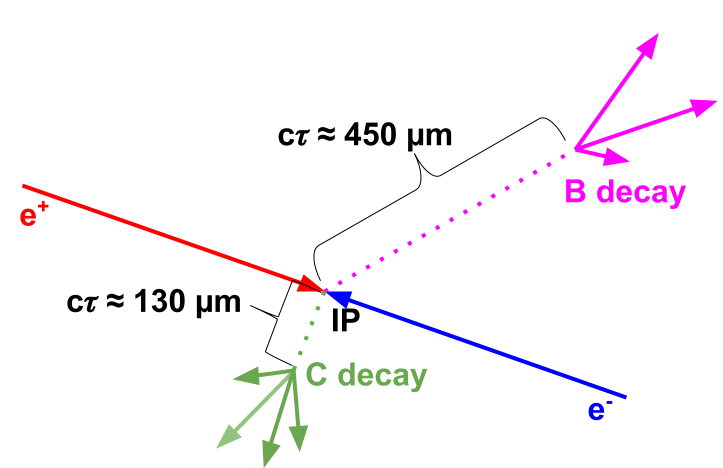
\includegraphics[width = \textwidth]{Pictures/ImpactParameter.png}
          \end{center}
        \end{column}
        \begin{column}{5cm}
          \centering
          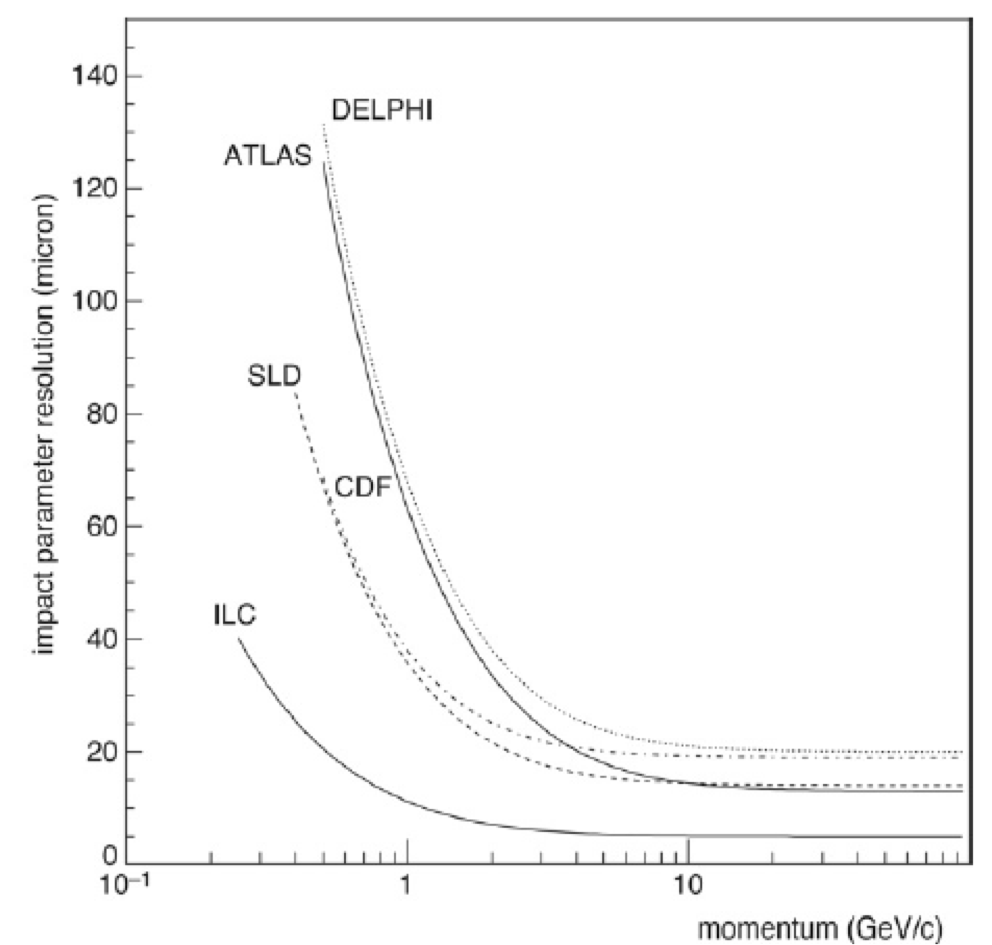
\includegraphics[width = 0.9\textwidth]{Pictures/IPresolution_variousColliders.png}
        \end{column}
      \end{columns}
    \end{block}

\end{frame}

%\subsection{Main aims}
%-------------------------------
%                           Aims
%-------------------------------

\begin{frame}
  \frametitle{ILD vertex detector}

  \vspace{-0.3cm}
  \begin{alertblock}{Impact parameter resolution}
      \centering{ $\sigma_{r\phi} \simeq \sigma_{rz} \simeq a \oplus \frac{b}{p \cdot sin^{2/2} \theta}$}
    \begin{itemize}
      \item Hit resolution: $a \simeq 4~\mu m \Rightarrow ~ \sigma_{spatial} < 3~\mu m$
      \item Multiple scattering: $b \simeq 9 - 15~\mu m \Rightarrow$ material budget per measurement point $\simeq 0.15~\%$ X$_0$ 
    \end{itemize}
  \end{alertblock}

  \vspace{-0.2cm}
  \begin{block}{Double-sided layer concept}
    \begin{columns}[c]
      \begin{column}{3cm}
        \vspace*{-0.1cm}
        \centering
        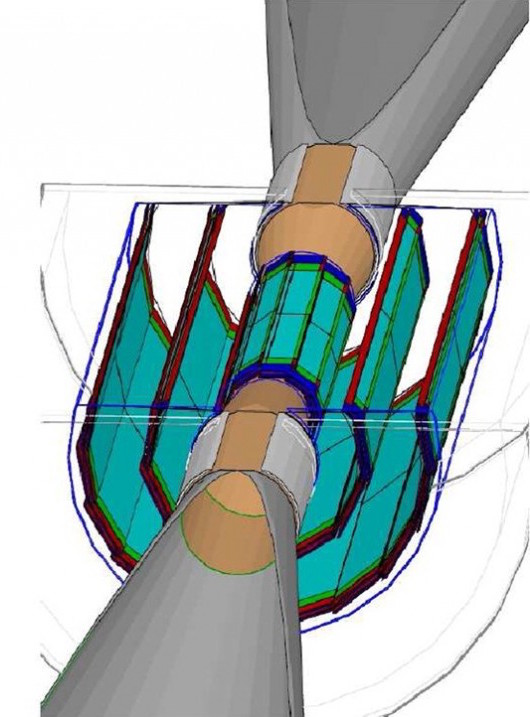
\includegraphics[width = 3cm]{Pictures/ild_vxd_3layers.jpg}
      \end{column}
      \begin{column}{7cm}
        %\vspace{-4cm}
        \centering
        \begin{itemize}
          \item 1 mechanical structure for \\ 2 measurement points
          \item Alignment
          \item Possibility to use 2 different technologies
        \end{itemize}
      \end{column}
    \end{columns}
  \end{block}

\end{frame}

%\begin{frame}
%  \frametitle{Main aims}
%
%  \begin{itemize}
%    \item \only<1>{Constraint material budget $\Rightarrow$ $< 0.3~\%$ X$_0$} \only<2>{\textbf{Constraint material budget} $\Rightarrow$ $< 0.3~\%$ X$_0$}
%    \item \only<1>{Study impact of the mechanical structure on sensor performance} \only<2>{\textbf{Study impact of the mechanical structure on sensor performance}}
%    \item Study the added value of double-sided measurement (\hyperlink{miniVec}{mini vectors})
%  \end{itemize}
%\end{frame}



%--------------------------------
%       PART I: PLUME

\begin{frame}
  \frametitle{Double-sided VXD: PLUME}

  \begin{columns}[c]
    \begin{column}{3cm}
      
\includegraphics[width = 3cm]{Pictures/logo_plume.png}
    \end{column}
    \vspace{-0.2cm}
    \begin{column}{7cm}
      PLUME = \textbf{P}ixelated \textbf{L}adder with \textbf{U}ltra-low \textbf{M}aterial \textbf{E}mbedding
    \end{column}
  \end{columns}

  \begin{columns}[t]
    \begin{column}{1cm}
      
\includegraphics[width = 1.5cm]{Pictures/logo_IPHC_10cm.png}
    \end{column}
    \begin{column}{1cm}
      
\includegraphics[width = 1cm]{Pictures/DESY-Logo.png}
    \end{column}
    \begin{column}{1cm}
      
\includegraphics[width = 2cm]{Pictures/logo_uni_bristol.jpg}
    \end{column}
  \end{columns}

  \vspace{-0.15cm}

  \begin{block}{Motivation}
    To build double-sided ladder with a geometry adapted for the ILD vertex detector at the ILC
  \end{block}

  \begin{block}{Goals}
    \begin{itemize}
      \item Reach a constraint material budget < $0.3~\%$ X$_0$
      \item Study the added values of double-sided measurement
      \item Study the mechanical structure and its impact on sensors' performance
    \end{itemize}
  \end{block}

  %\vspace{-0.18cm}
  %\begin{block}{Design}
  %  \begin{itemize}
  %    \item Double-sided ladder with an active area of 1x12cm$^2$
  %    \item On each side: six MIMOSA-26 CMOS sensors thinned down to $\sim 50~\mu$m on a kapton-metal flex cable
  %    \item 2 mm of silicon carbide foam as mechanical support and spacer between two modules
  %  \end{itemize}
  %\end{block}
\end{frame}

\subsection{Design}
%-------------------------------
%                           PLUME scheme + picture of a module
%-------------------------------

\begin{frame}
  \frametitle{What does it look like?}

  \vspace{-0.2cm}
  \begin{center}
    %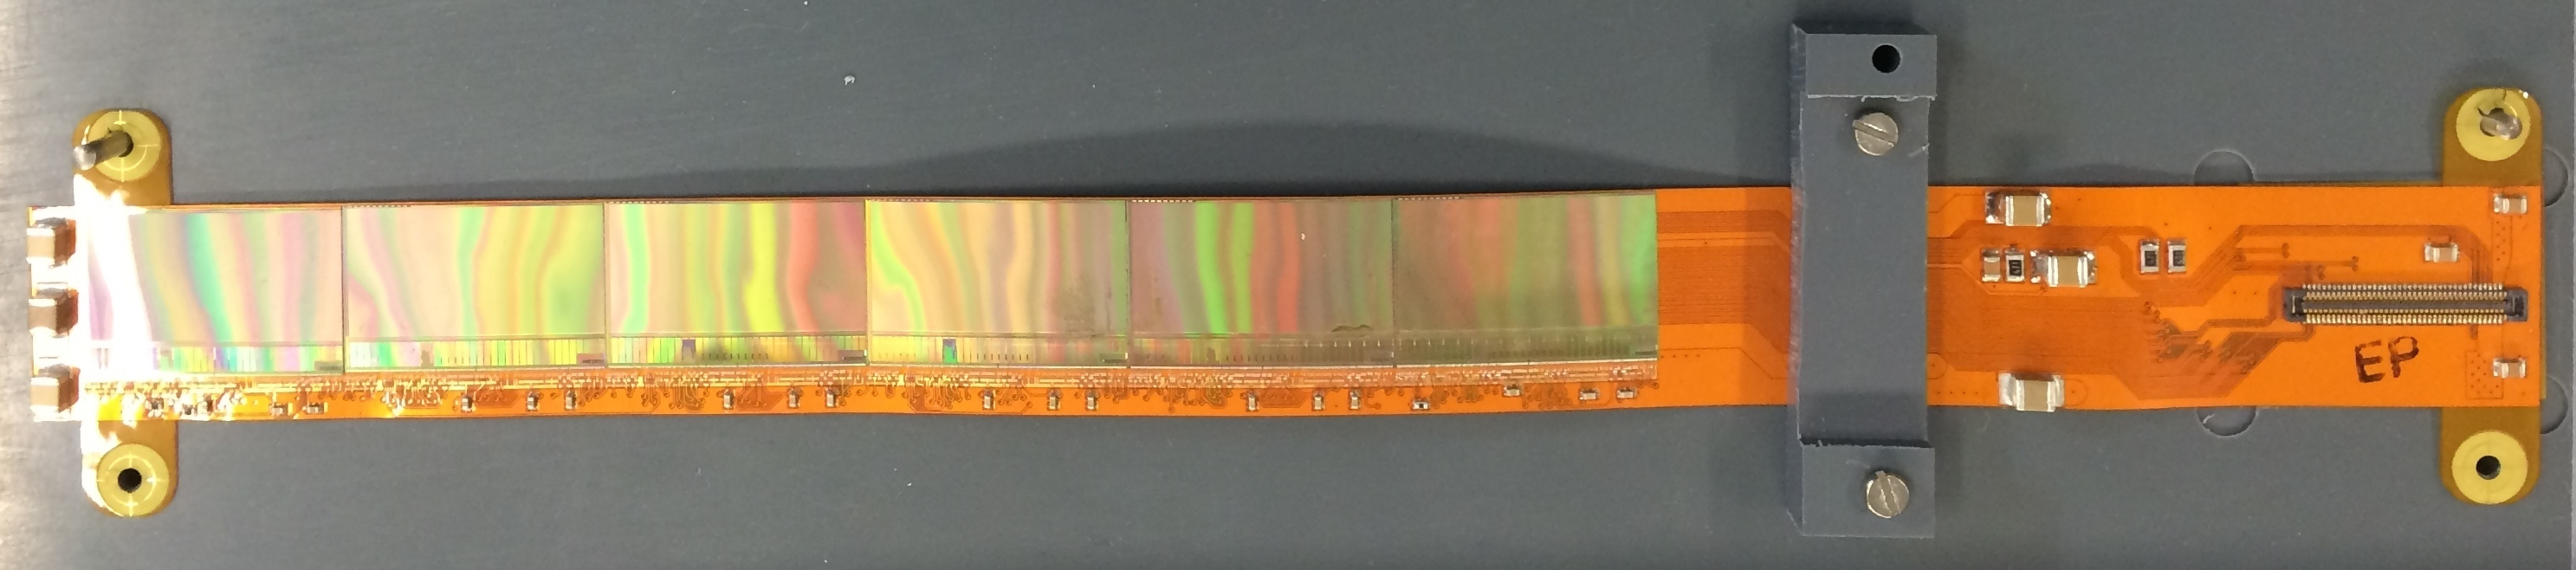
\includegraphics[width = 10 cm]{Pictures/PLUME_copper_module.png}
    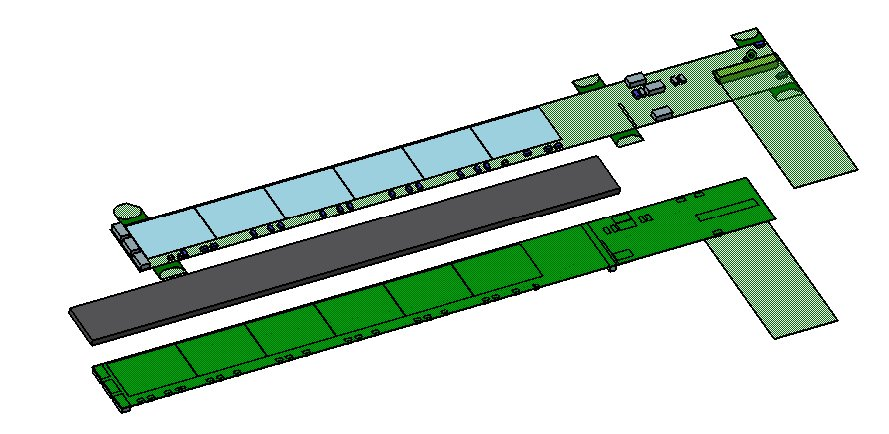
\includegraphics[width = 0.8\textwidth]{Pictures/Plume2_vue_eclatee.jpg}

    %Picture of one module with copper traces.
  \end{center}

  \vspace{-0.2cm}
  \begin{center}
    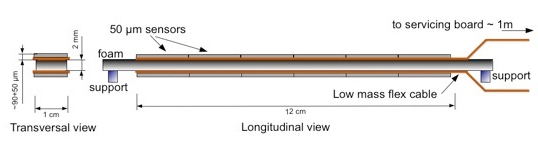
\includegraphics[width = 10 cm]{Pictures/scheme_plume.png}

    %Scheme of one PLUME ladder.
  \end{center}
\end{frame}

%-------------------------------
%                           FOAM
%-------------------------------

\begin{frame}
  \frametitle{PLUME in real}

  \begin{center}
    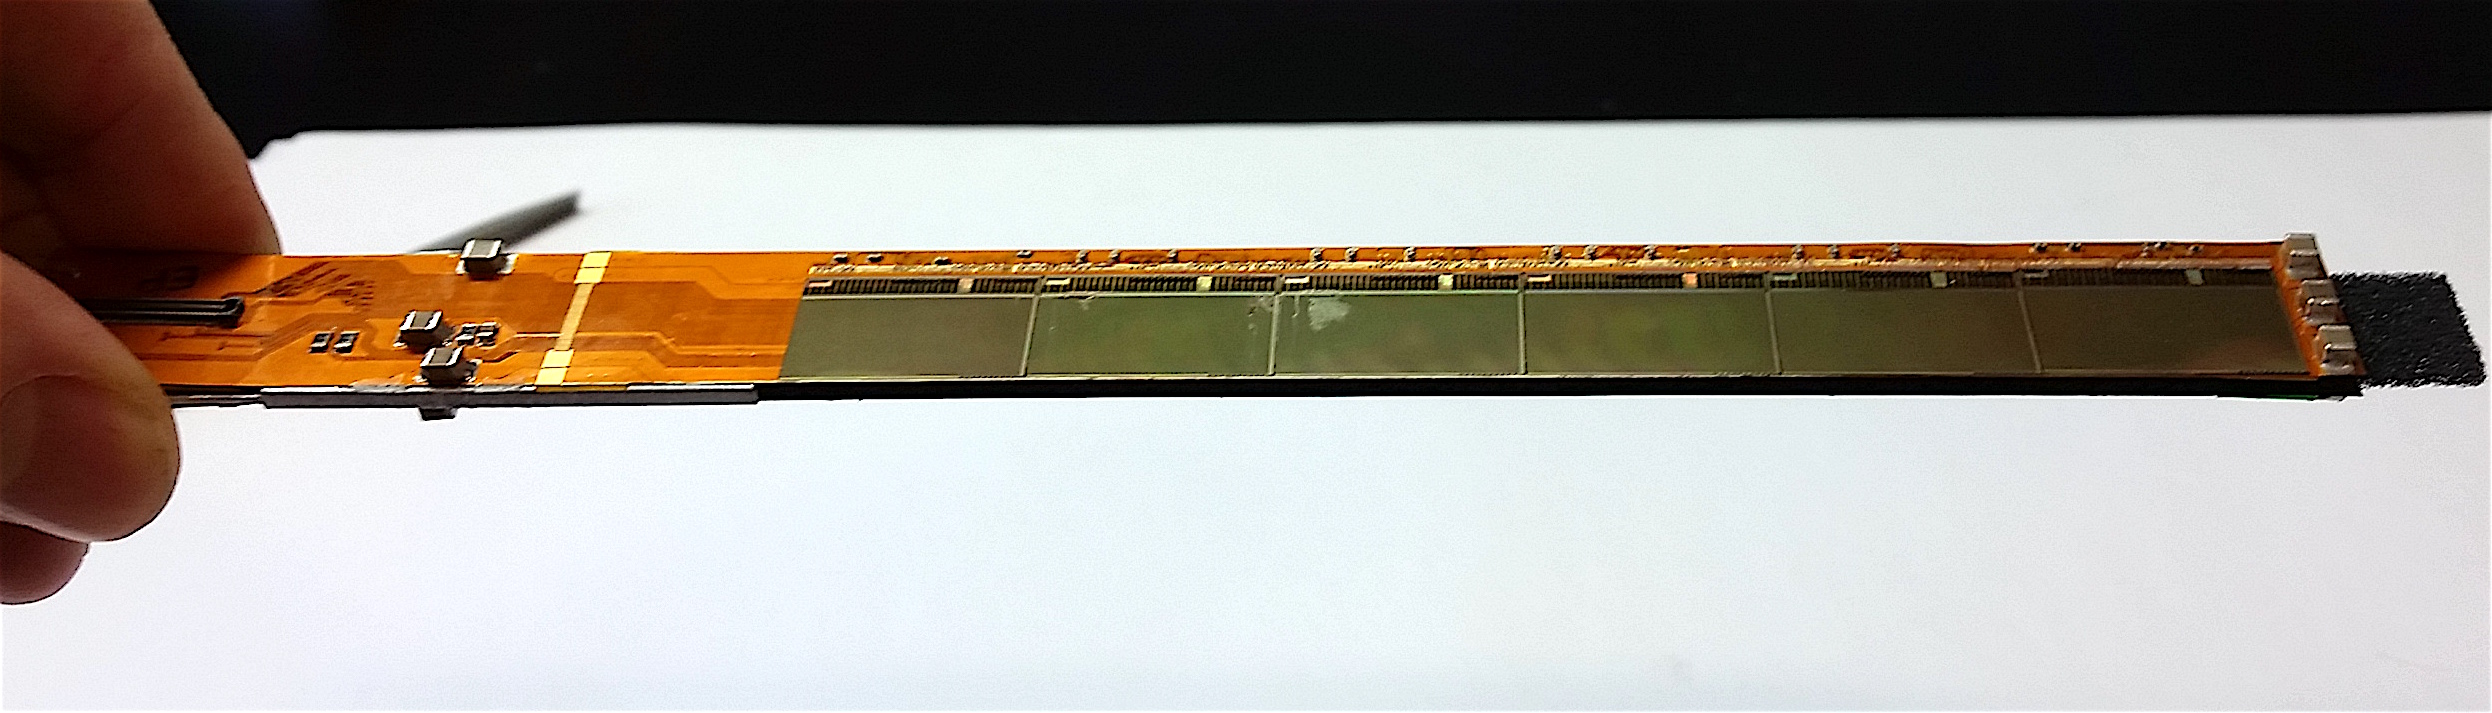
\includegraphics[width = \textwidth]{Pictures/plume2.jpg}
  \end{center}
  
  \begin{columns}{t}
    \begin{column}{0.5\textwidth}
      \centering
      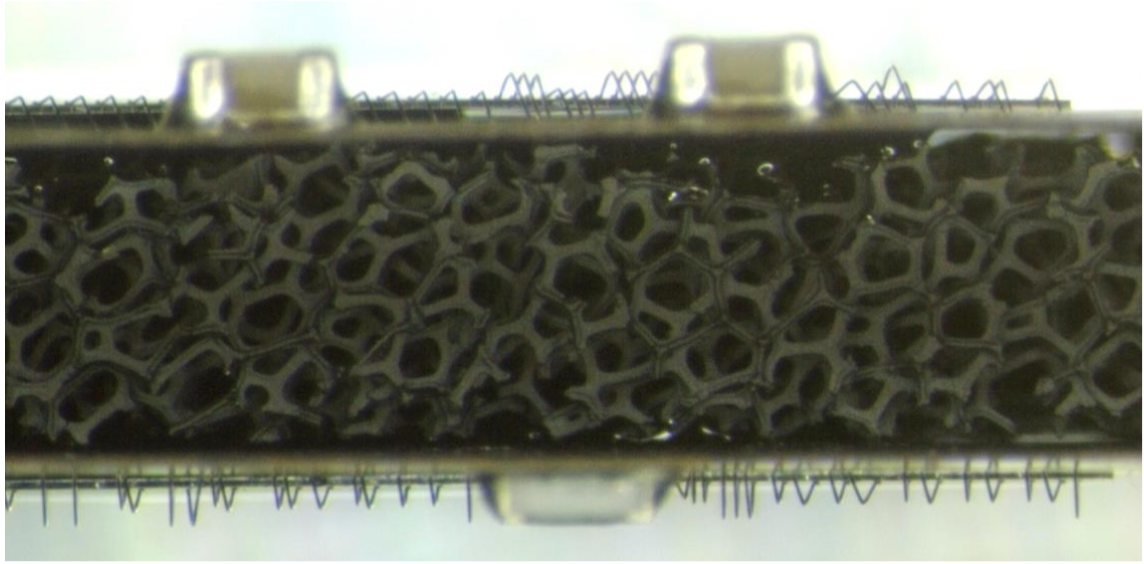
\includegraphics[width = \textwidth]{Pictures/SiC.png}
    \end{column}
    \begin{column}{0.5\textwidth}
      \begin{itemize}
        \item $2~\text{mm}$ SiC foam
        \item $50~\mu\text{m}$ CMOS pixel sensor
        \item $100~\mu\text{m}$ flex-cable
        \item Air-flow cooling system
      \end{itemize}
    \end{column}
  \end{columns}
\end{frame}

%-------------------------------
%                           Mi26 
%-------------------------------

\begin{frame}
  \frametitle{MIMOSA-26 sensor}

  \vspace{-0.5cm}
  \begin{columns}[c]
    \begin{column}{4cm}
      \begin{center}
        %\vspace{-0.3cm}
        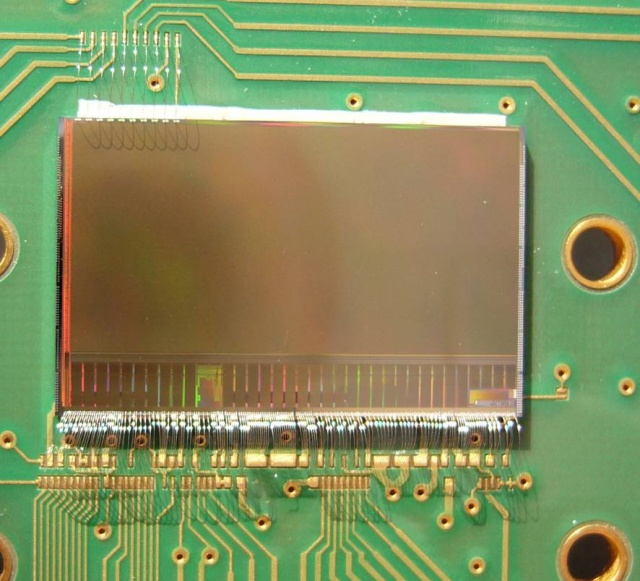
\includegraphics[width = 4.0cm,height=3.6cm]{Pictures/mi26.jpg}
      \end{center}
    \end{column}

    \begin{column}{4cm}
      \vspace{-0.3cm}
      \begin{center}
        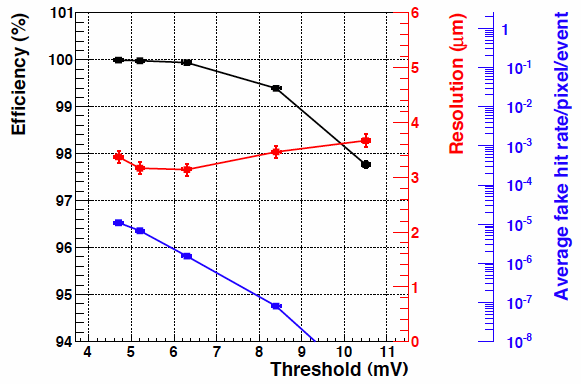
\includegraphics[width = 4.5cm]{Pictures/MIMOSA26_chip26_HR15_20deg.png}

        % \tiny{From IPHC - Strasbourg}
      \end{center}
      %    \begin{center}
      %        \begin{block}{Well known chips}
      %        Used for EUDET style telescopes since 2009
      %        \end{block}
      %    \end{center}
    \end{column}
    \begin{column}{4cm}
      \begin{center}
        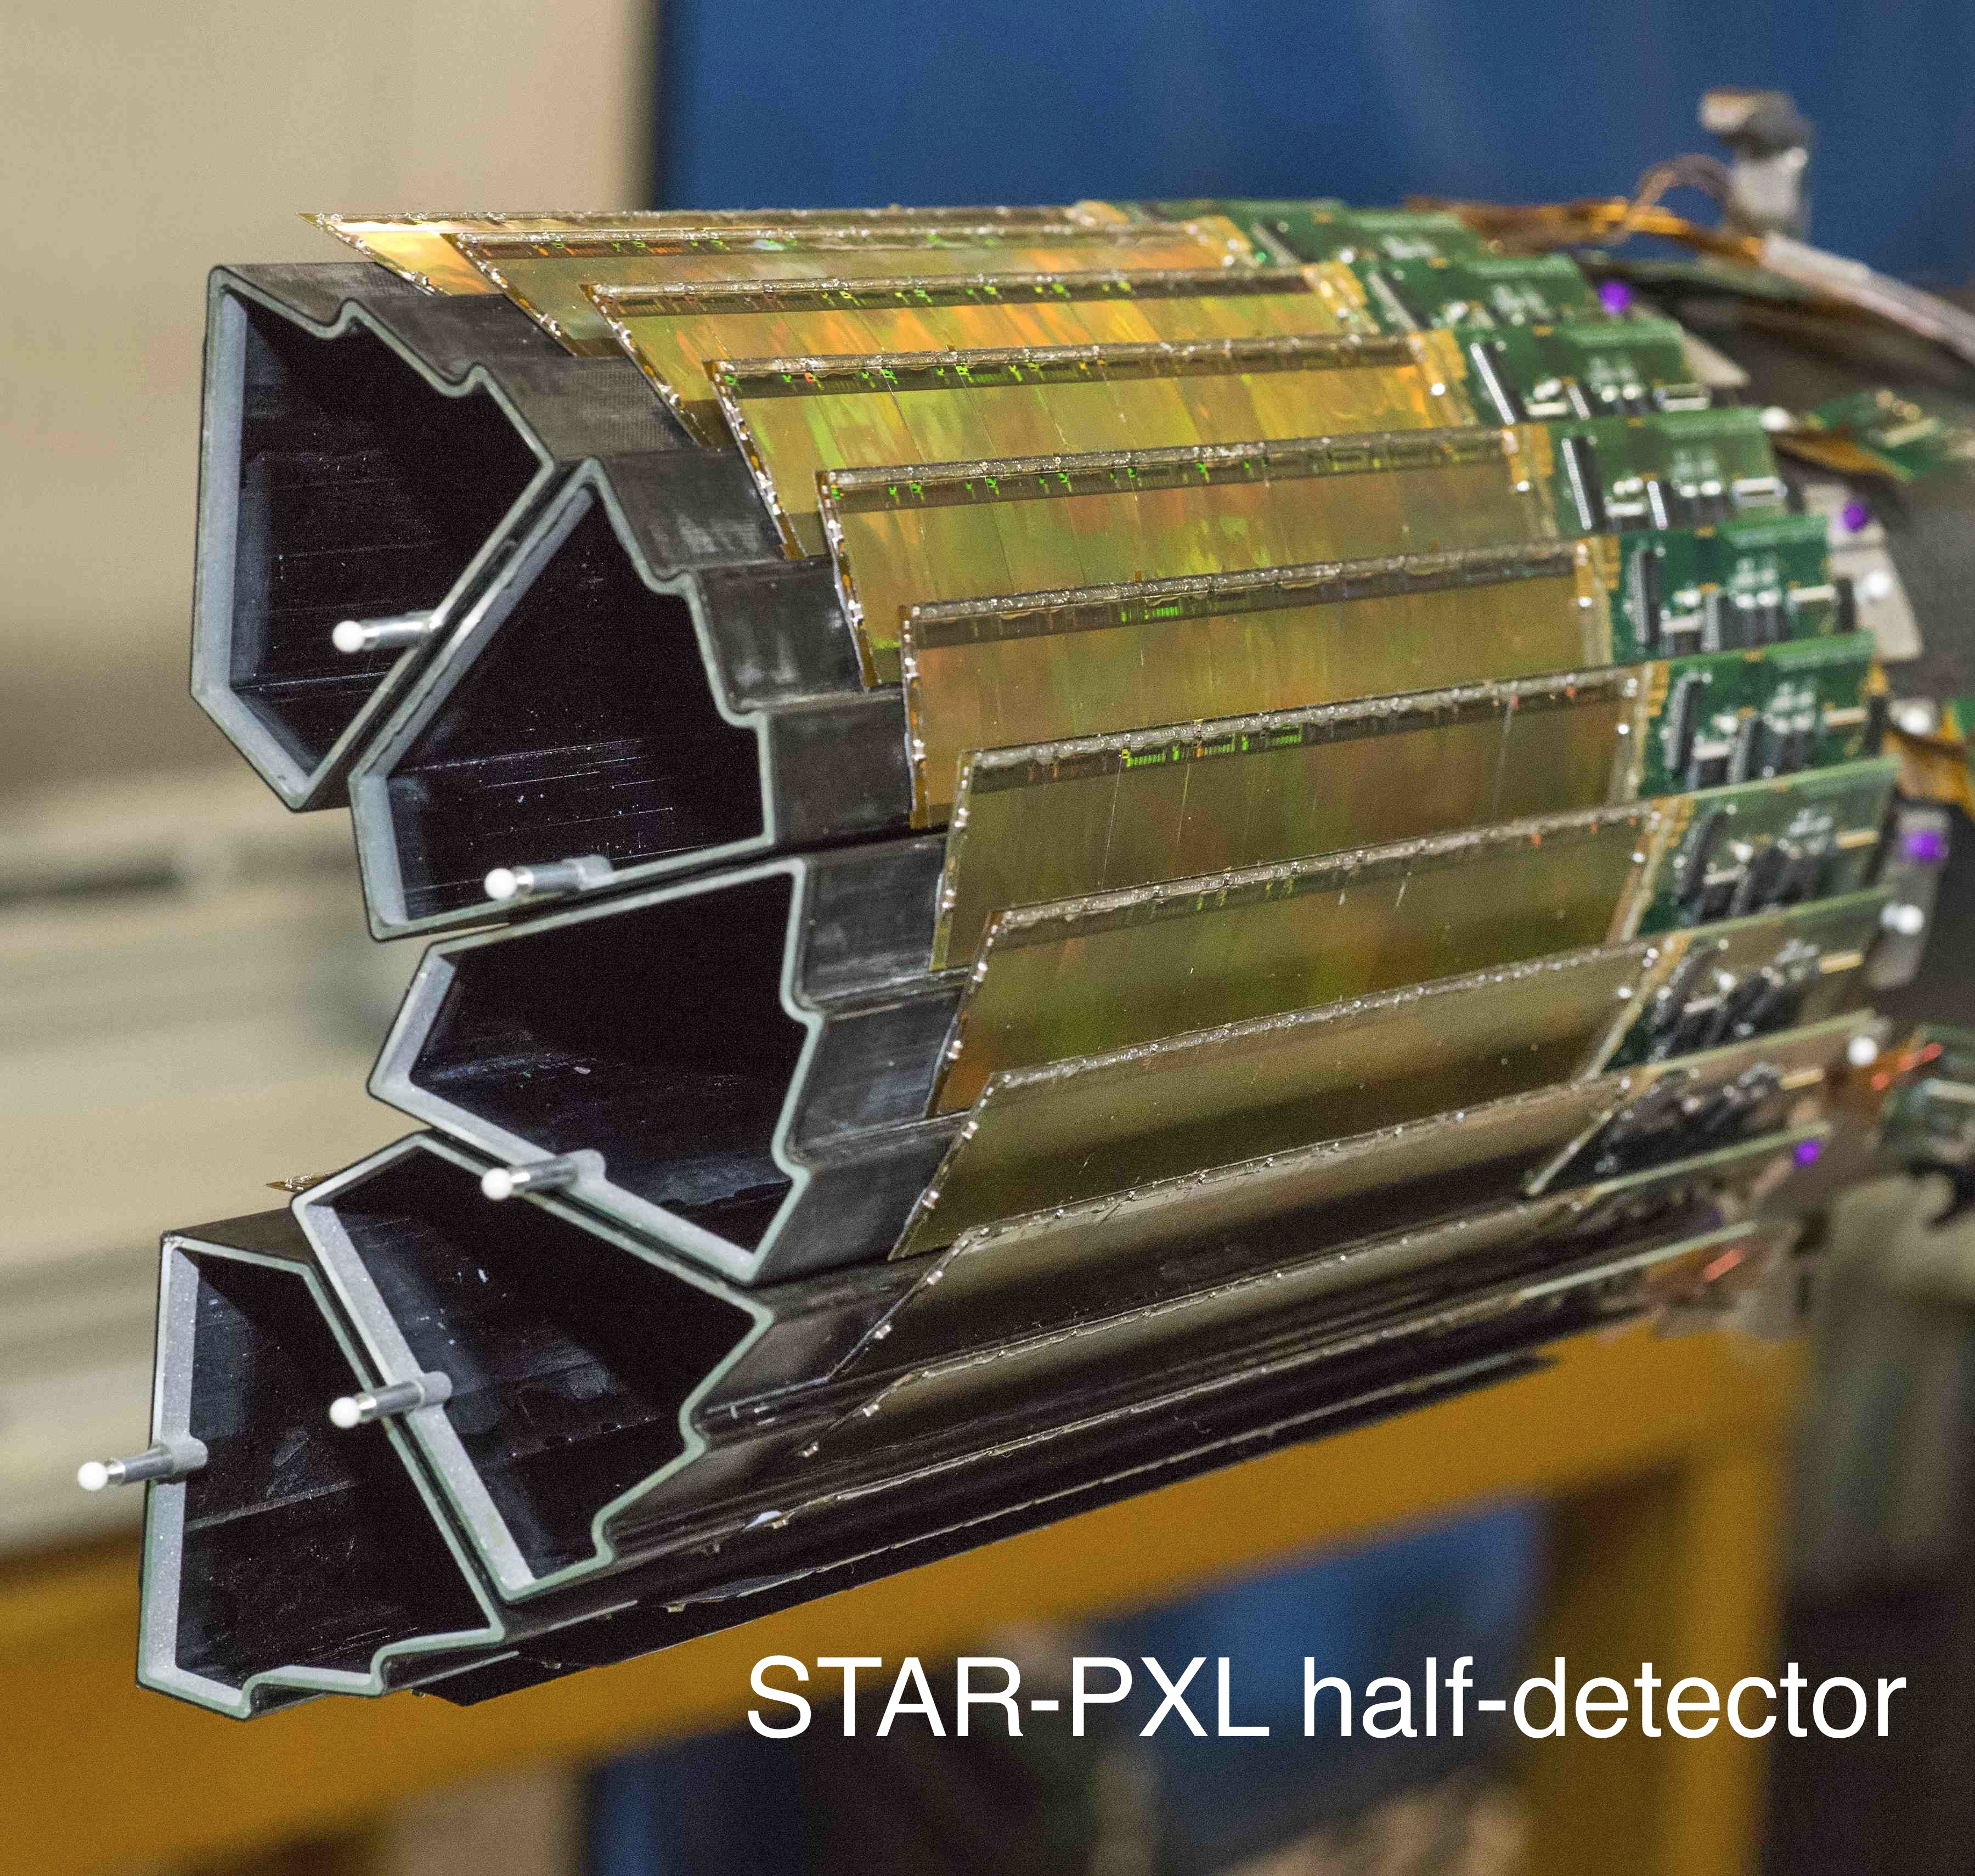
\includegraphics[width = 4.0cm, height=3.6cm]{Pictures/pxlFinal_sideView_smallSize.jpg}
      \end{center}
    \end{column}
  \end{columns}

  \vspace{-0.2cm}
  \begin{block}{Monolithic Active Pixels Sensor (MAPS)}
    \scriptsize{
    \begin{itemize}
      \item Well known sensors $\Rightarrow$ used for EUDET telescope
      \item Extended to MIMOSA-28 exploited in STAR-PXL vertex detector @ RHIC-BNL since 2014
      \item Thickness: $50~\mu\text{m}$
      \item Pitch: $18.4~\mu\text{m}$ (square pixels)
      \item Active area: $10.6 \times 21.2 \text{mm}^2$ (576 rows x 1152 columns)
      \item Integration time: $115.2~\mu\text(s)$ ($200~\text{ns}$ per line)
      \item Binary output with \hyperlink{suze}{Zero suppression}
    \end{itemize}
   }
  \end{block}

  %\vspace{-0.2cm}
  %\scriptsize{
  %  \begin{itemize}
  %    \item Monolithic Active Pixels Sensor 
  %    \item Pitch of 18.4 $\mu m$ (square pixels)
  %    \item Active area: 10.6 x 21.2 mm$^2$ (576 rows x 1152 columns)
  %    \item Column-parallel readout: integration time of 115.2 $\mu$s (200 ns per line) for 80 MHz clock
  %    \item \hyperlink{suze}{Zero suppression} (to optimize data bandwith) with binary output
  %    \item Well known sensors $\Rightarrow$ used for EUDET telescope
  %    \item Extended to MIMOSA-28 exploited in STAR-PXL vertex detector @ RHIC-BNL since 2014
  %  \end{itemize}
  %}
  %\grille
\end{frame}

  \subsection{Test beam}

  \begin{frame}
    \frametitle{Test beam}

    \begin{block}{Motivation}
      Test detector under real conditions to determine its performance
    \end{block}
      
    \begin{exampleblock}{Set-up}
      \centering
      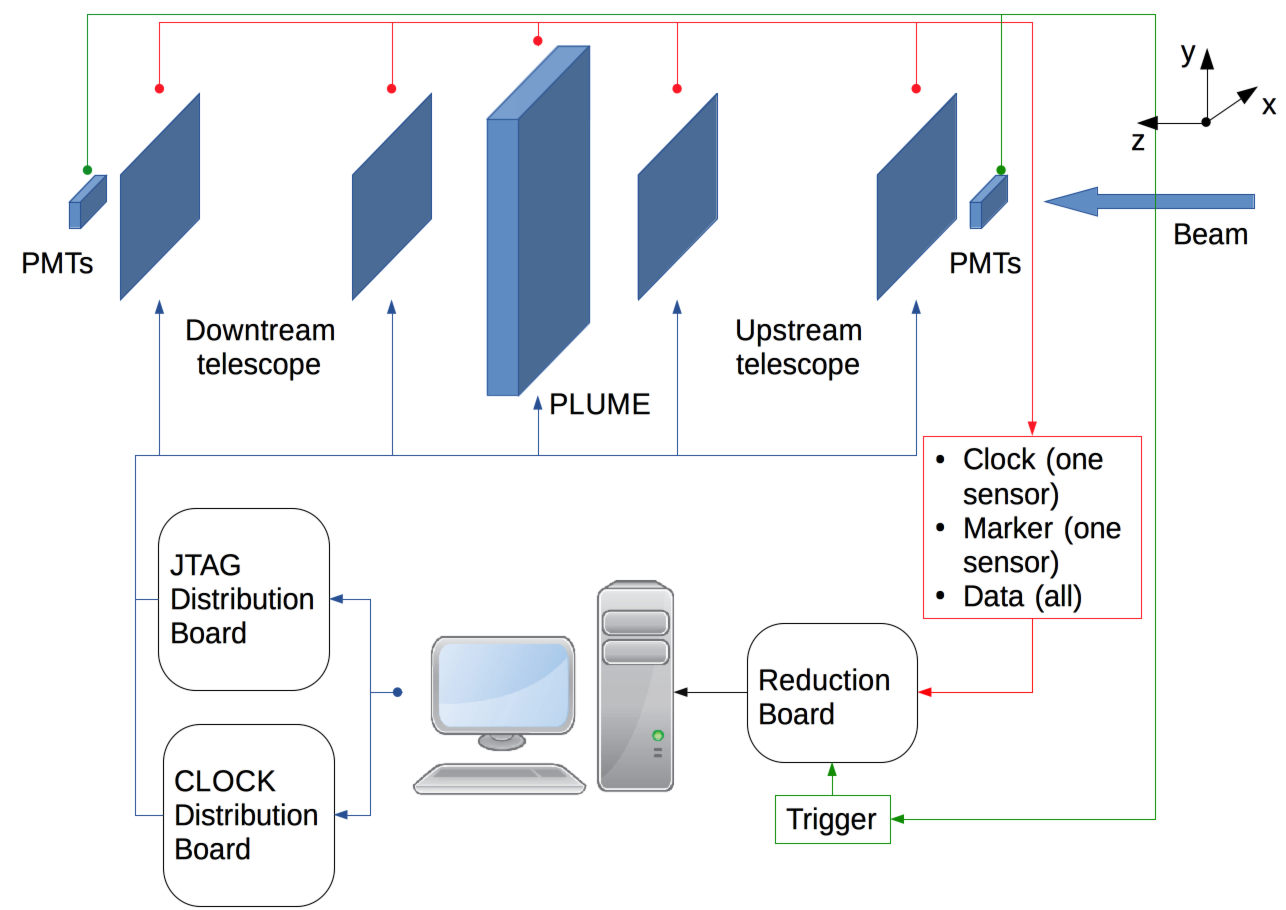
\includegraphics[width = 0.6\textwidth]{Pictures/testBeamAcquisition.png}
    \end{exampleblock}
  
  \end{frame}

\begin{frame}
    \frametitle{Track-hit residual}

    \begin{columns}[c]
    \hspace{-0.8cm}
      \begin{column}{7cm}
        \begin{flushleft}
          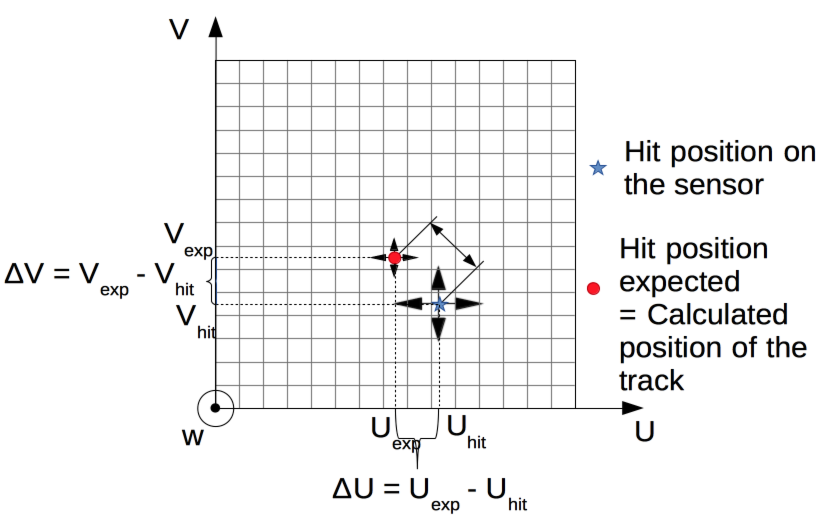
\includegraphics[width = 7cm]{Pictures/residual_explanation.png}
        \end{flushleft}
      \end{column}
    \hspace{-0.8cm}
      \begin{column}{4cm}
        \centering
        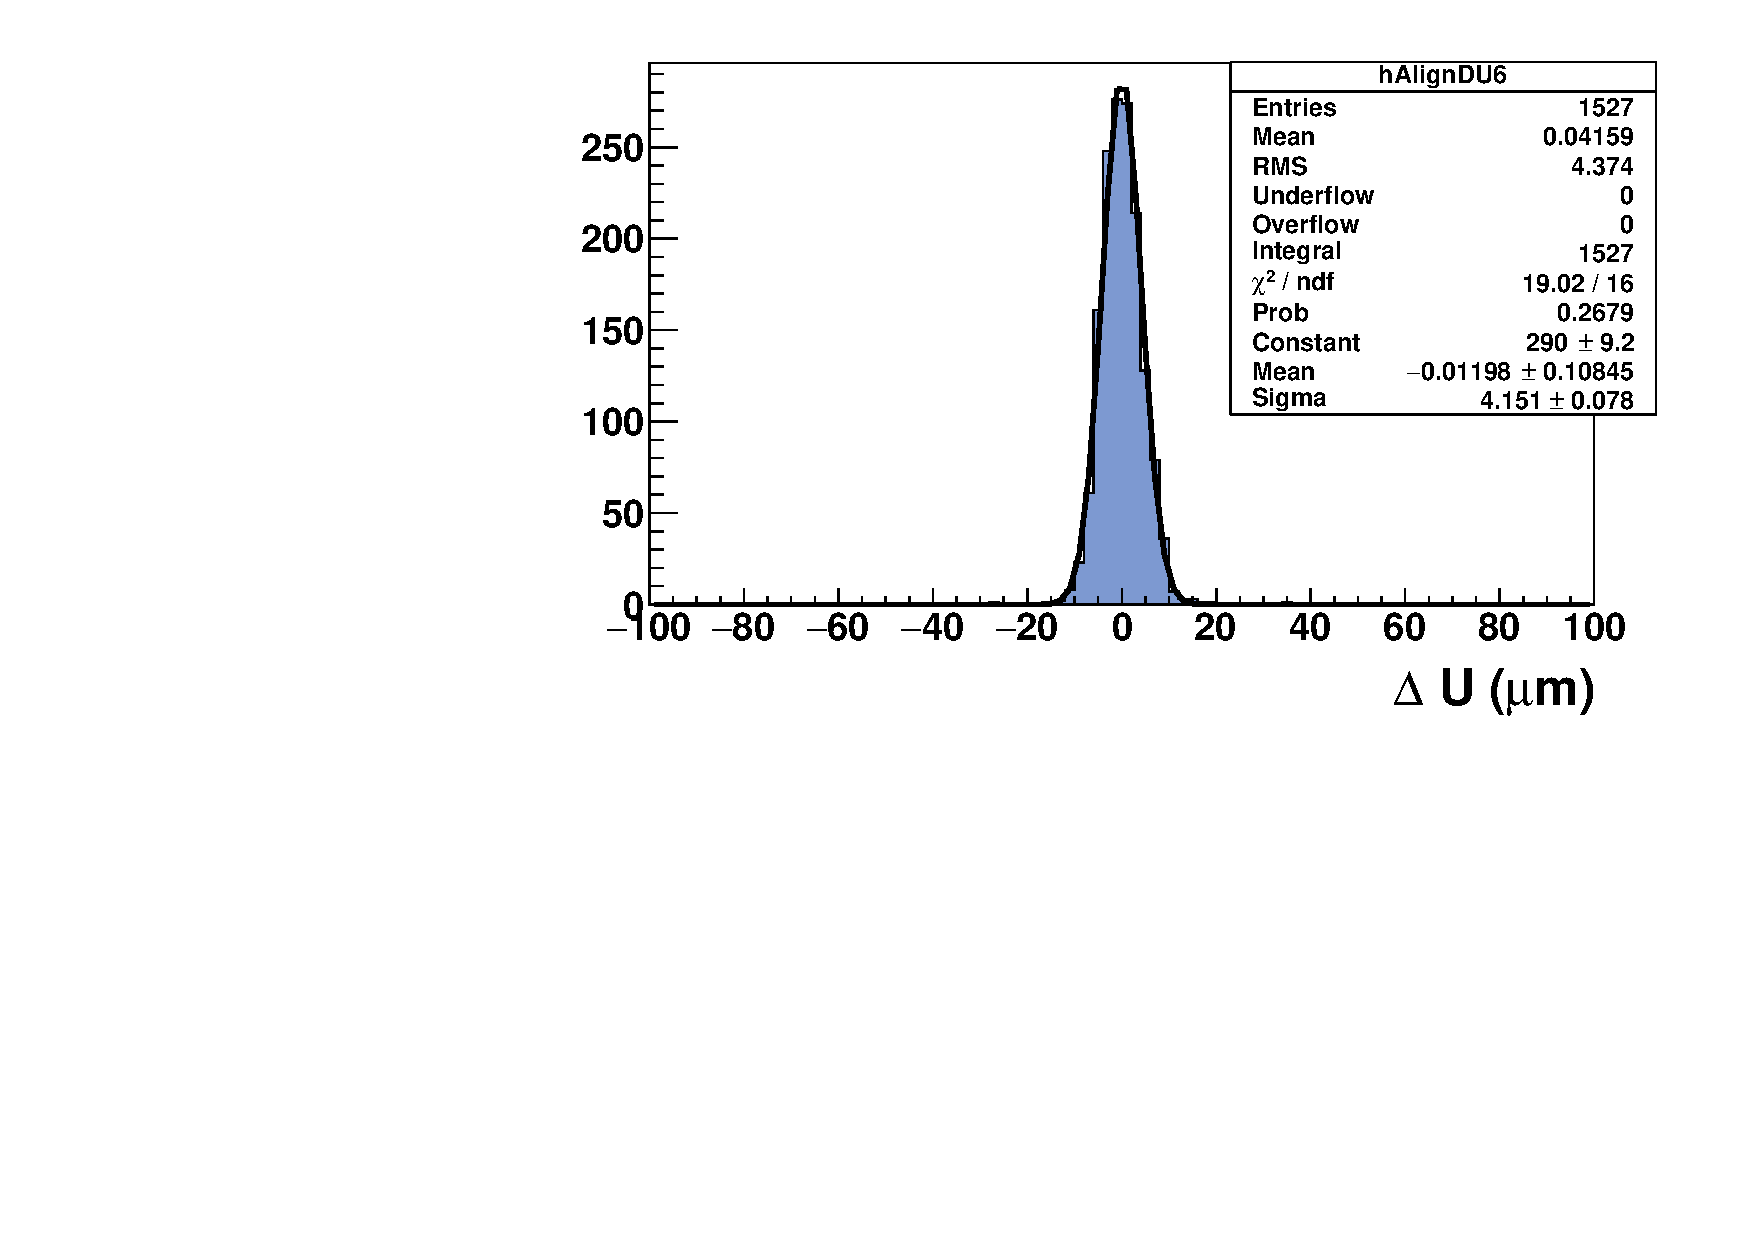
\includegraphics[width = 1.2\textwidth ]{Pictures/deltaU_6_normal_incidence.pdf}
      \end{column}
    \end{columns}
\end{frame}

\section{Mechanical deformation}
\begin{frame}
  \frametitle{Outlines}
  \begin{minipage}{\textwidth}
    \tableofcontents[currentsection,hideothersubsections, 
    sectionstyle=show/shaded]
  \end{minipage}
\end{frame}

  \subsection{Surface's survey}
  \begin{frame}
    \frametitle{Metrology of module's surface}

    \begin{block}{Are our ladders completely flat?}
     
     \begin{center}
        Peak-to-peak flatness $\sim 100~\mu$m
     \end{center}

      \vspace{-0.2cm}
      \begin{columns}[c]
        \begin{column}{5cm}
          \begin{center}
            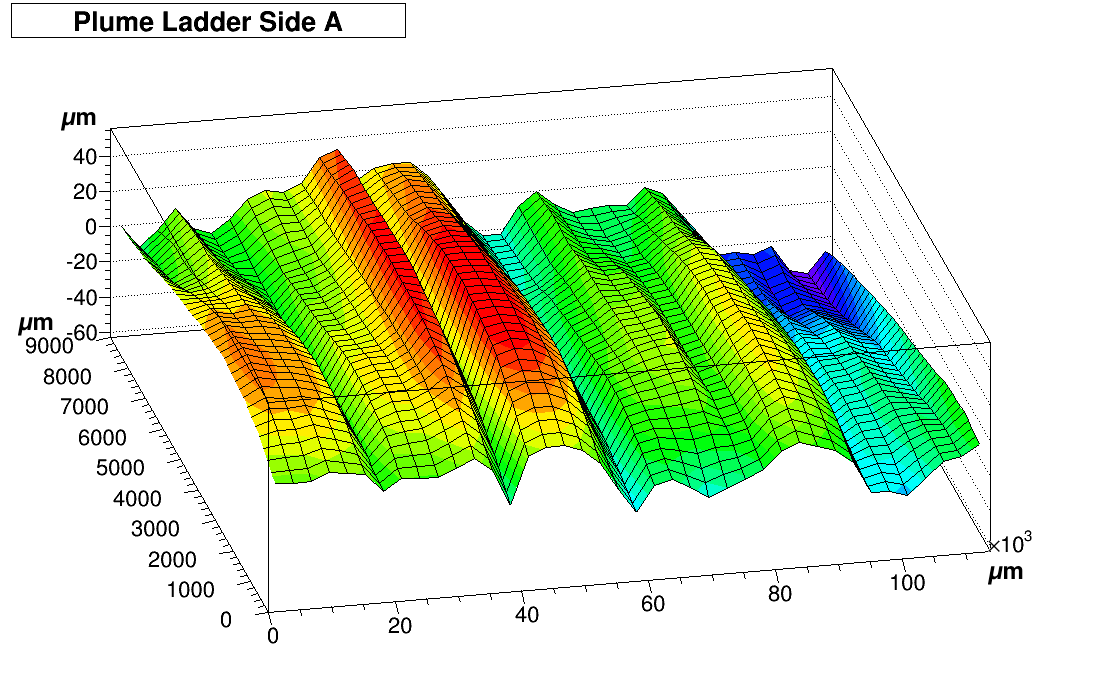
\includegraphics[width = 0.95\textwidth]{Pictures/SideAPlumeLadder2010_M20.png}
          \end{center}
        \end{column}

        \begin{column}{5cm}
          \begin{center}
            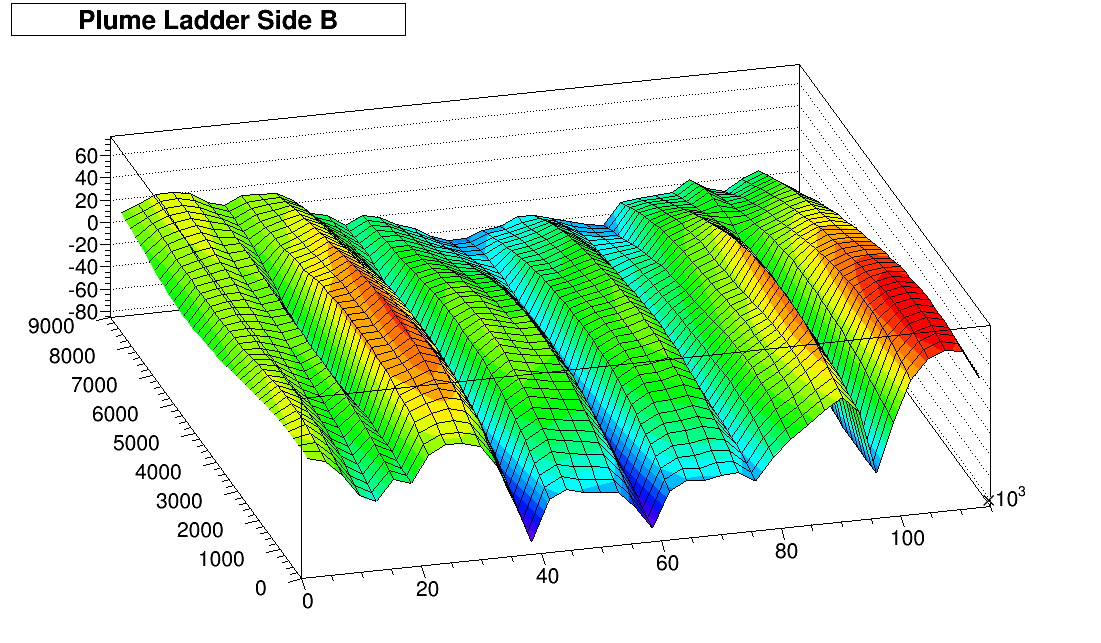
\includegraphics[width = \textwidth]{Pictures/SideBPlumeLadder2010_M20.png}
          \end{center}
        \end{column}
      \end{columns}
      
      \begin{center}

        \footnotesize{Test performed at Bristol with a dummy ladder}
      \end{center}

    \end{block}
    
    \begin{alertblock}{Question}
      What is the impact of such deformations on ladder's performance?
    \end{alertblock}
  \end{frame}

%-------------------------------
%   TB
%-------------------------------
  %\subsection{Test Beam @ SPS}
  \begin{frame}
    \frametitle{Test of the first fully functional prototype}
    %\frametitle{Test beam @ SPS with 120 GeV $\pi^-$ in November 2011}

    \vspace{-0.5cm}
    \begin{columns}[t]
      \begin{column}{4cm}
        \begin{center}
          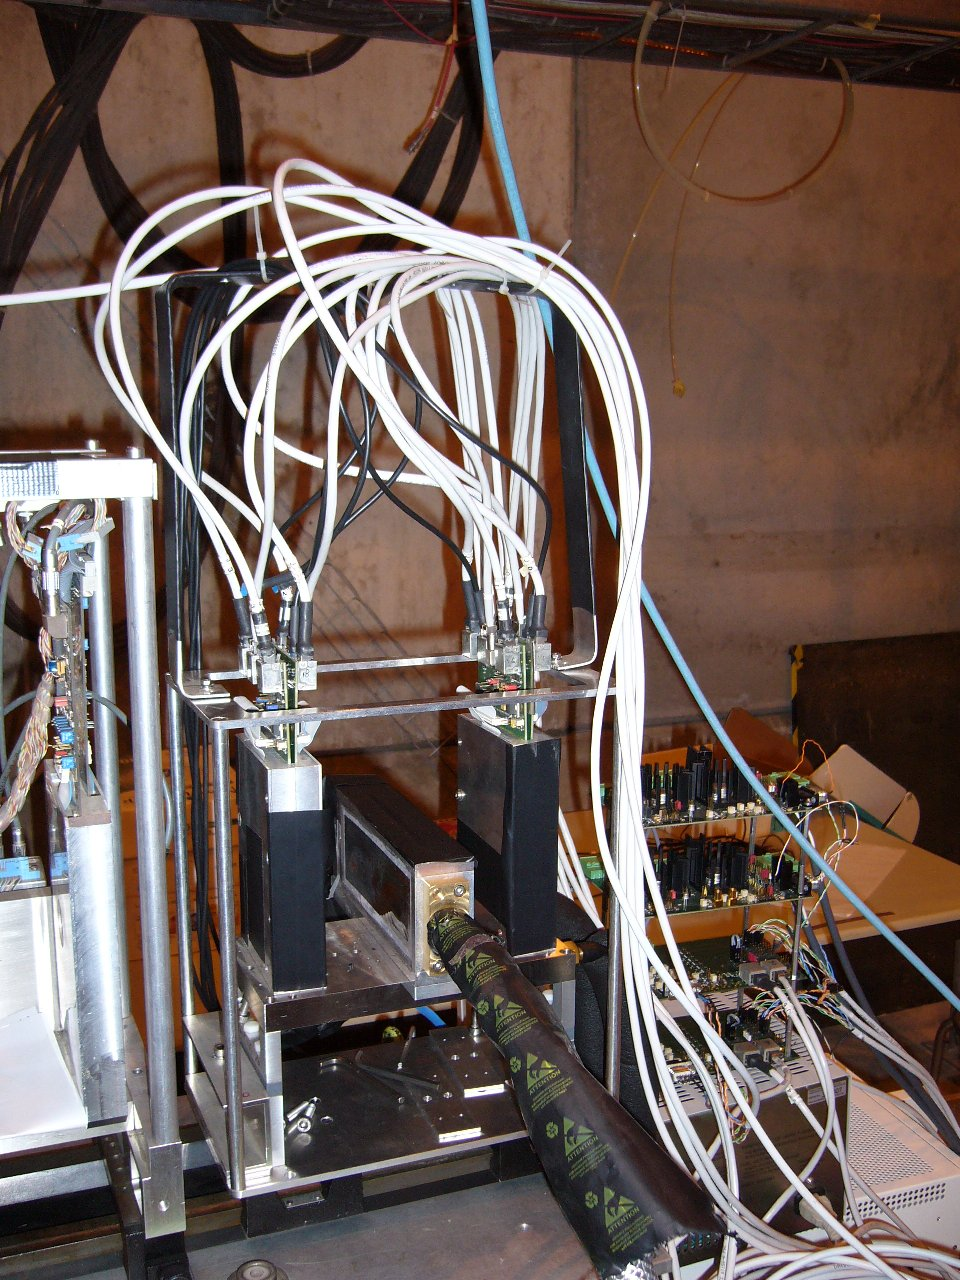
\includegraphics[width = 4 cm]{Pictures/plume_testBeam_nov2011.jpg}
        \end{center}
      \end{column}

      \begin{column}{7cm}
        \begin{block}{Test beam 2011}
          \footnotesize{
          \begin{itemize}
            \item CERN-SPS with 120 GeV $\pi^{-}$
            \item Reference plane: 4 MIMOSA-26
            \item DUT: first double-sided ladder equipped with 12 MIMOSA-26 sensors
            \item Ladder performance studies with different configurations
          \end{itemize}
          }
        \end{block}

        \vspace{-0.3cm}
        \begin{block}{Impact of deformations}
          \footnotesize{
          \begin{itemize}
            \item Already observed and studied by 2 Ph. D. students
            \item Method to correct manually and locally these deviations
          \end{itemize}
          }
        \end{block}
      \end{column}
    \end{columns}
          
    \centering{Is it possible to include the deformations observed during the offline analysis?}

    %\vspace{0.1cm}
    %\footnotesize{
    %\centering{Jérôme Baudot, Gilles Claus, Loic Cousin, Mathieu Goffe, Rohrry Gold, Joel Goldstein, Ingrid Gregor, Robert Maria.}}
  \end{frame}

  \begin{frame}
    \frametitle{Geometrical configurations studied}

    \vspace{-0.1cm}
    \begin{columns}[t]
      \begin{column}{4cm}
        \begin{center}
          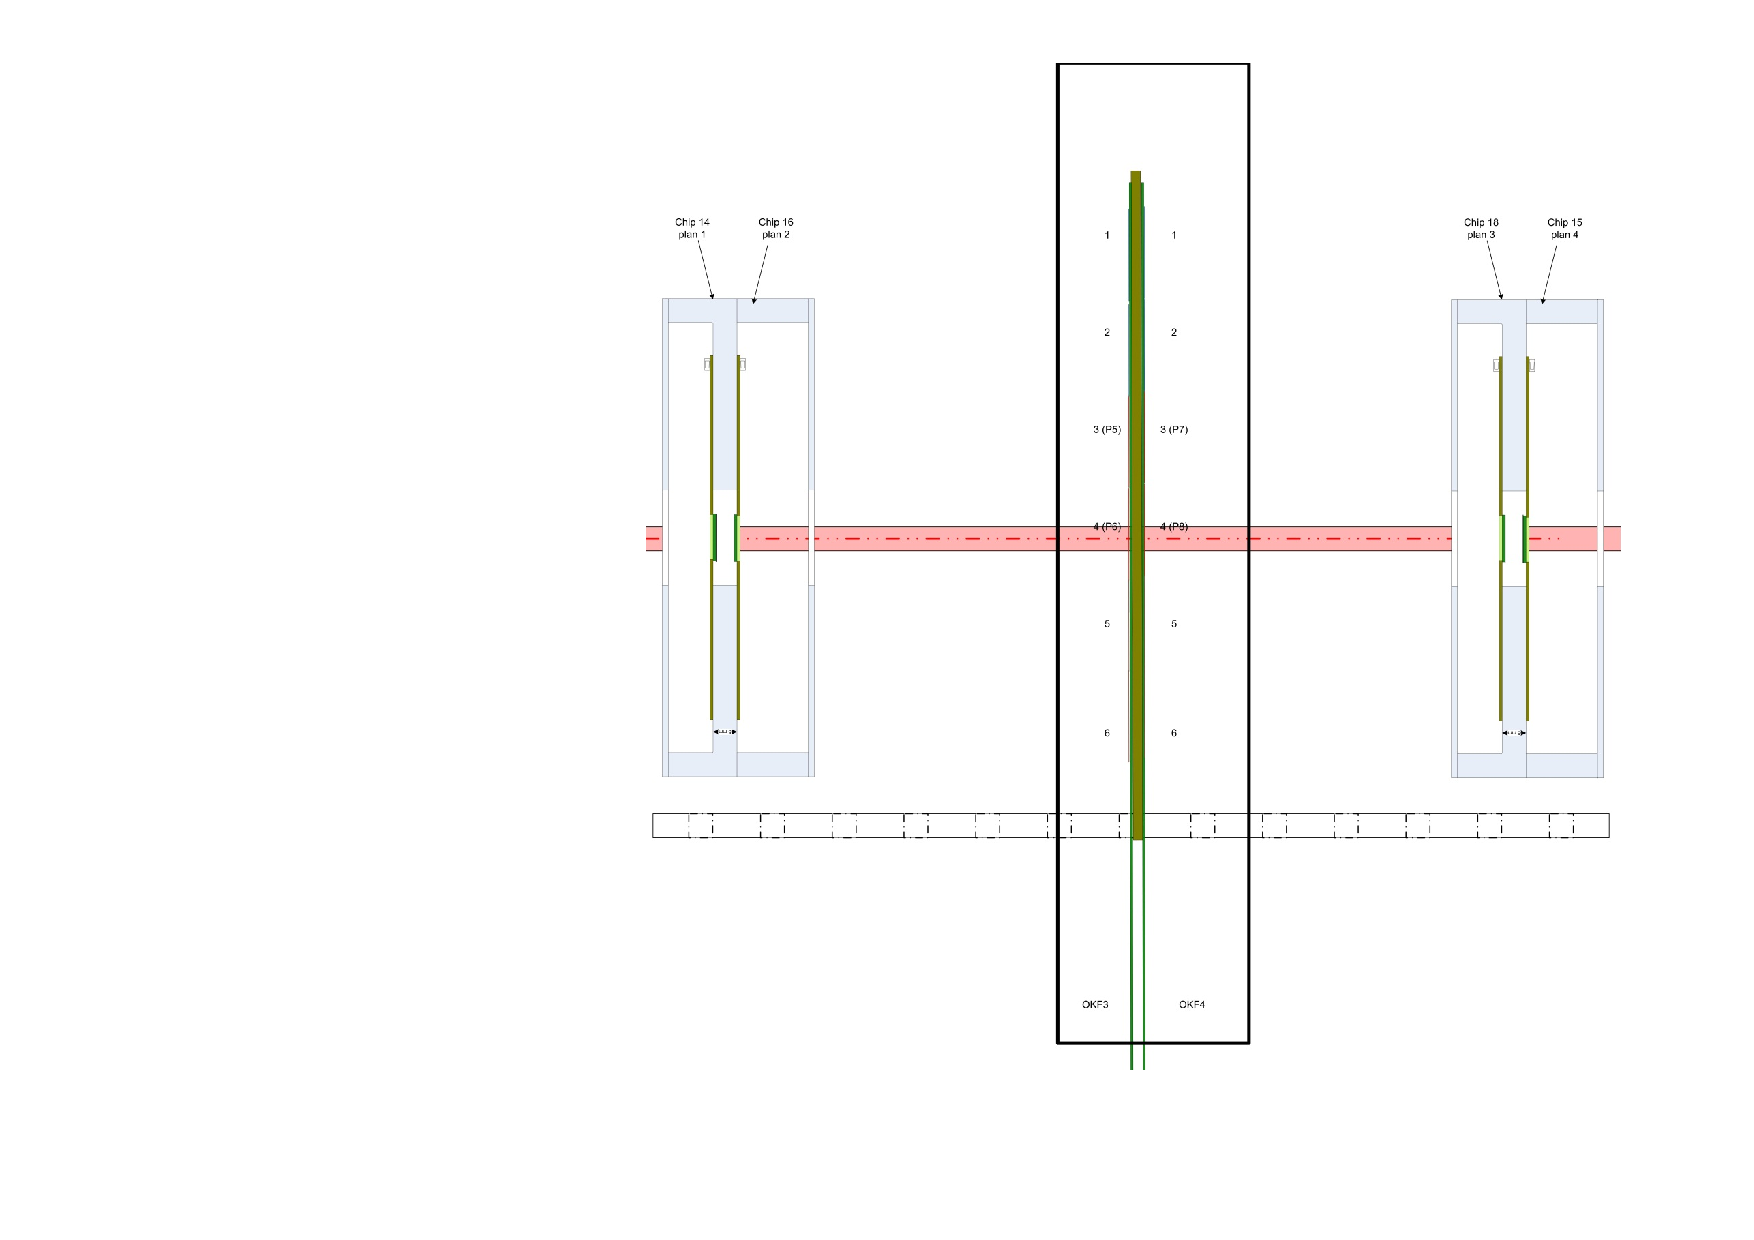
\includegraphics[width = 4cm,height = 3.9cm]{Pictures/tb_cern_11_sketch_normal.pdf}

          \footnotesize{\textbf{Module perpendicular to the beam.}}
        \end{center}
      \end{column}

      \begin{column}{4cm}
        \begin{center}
          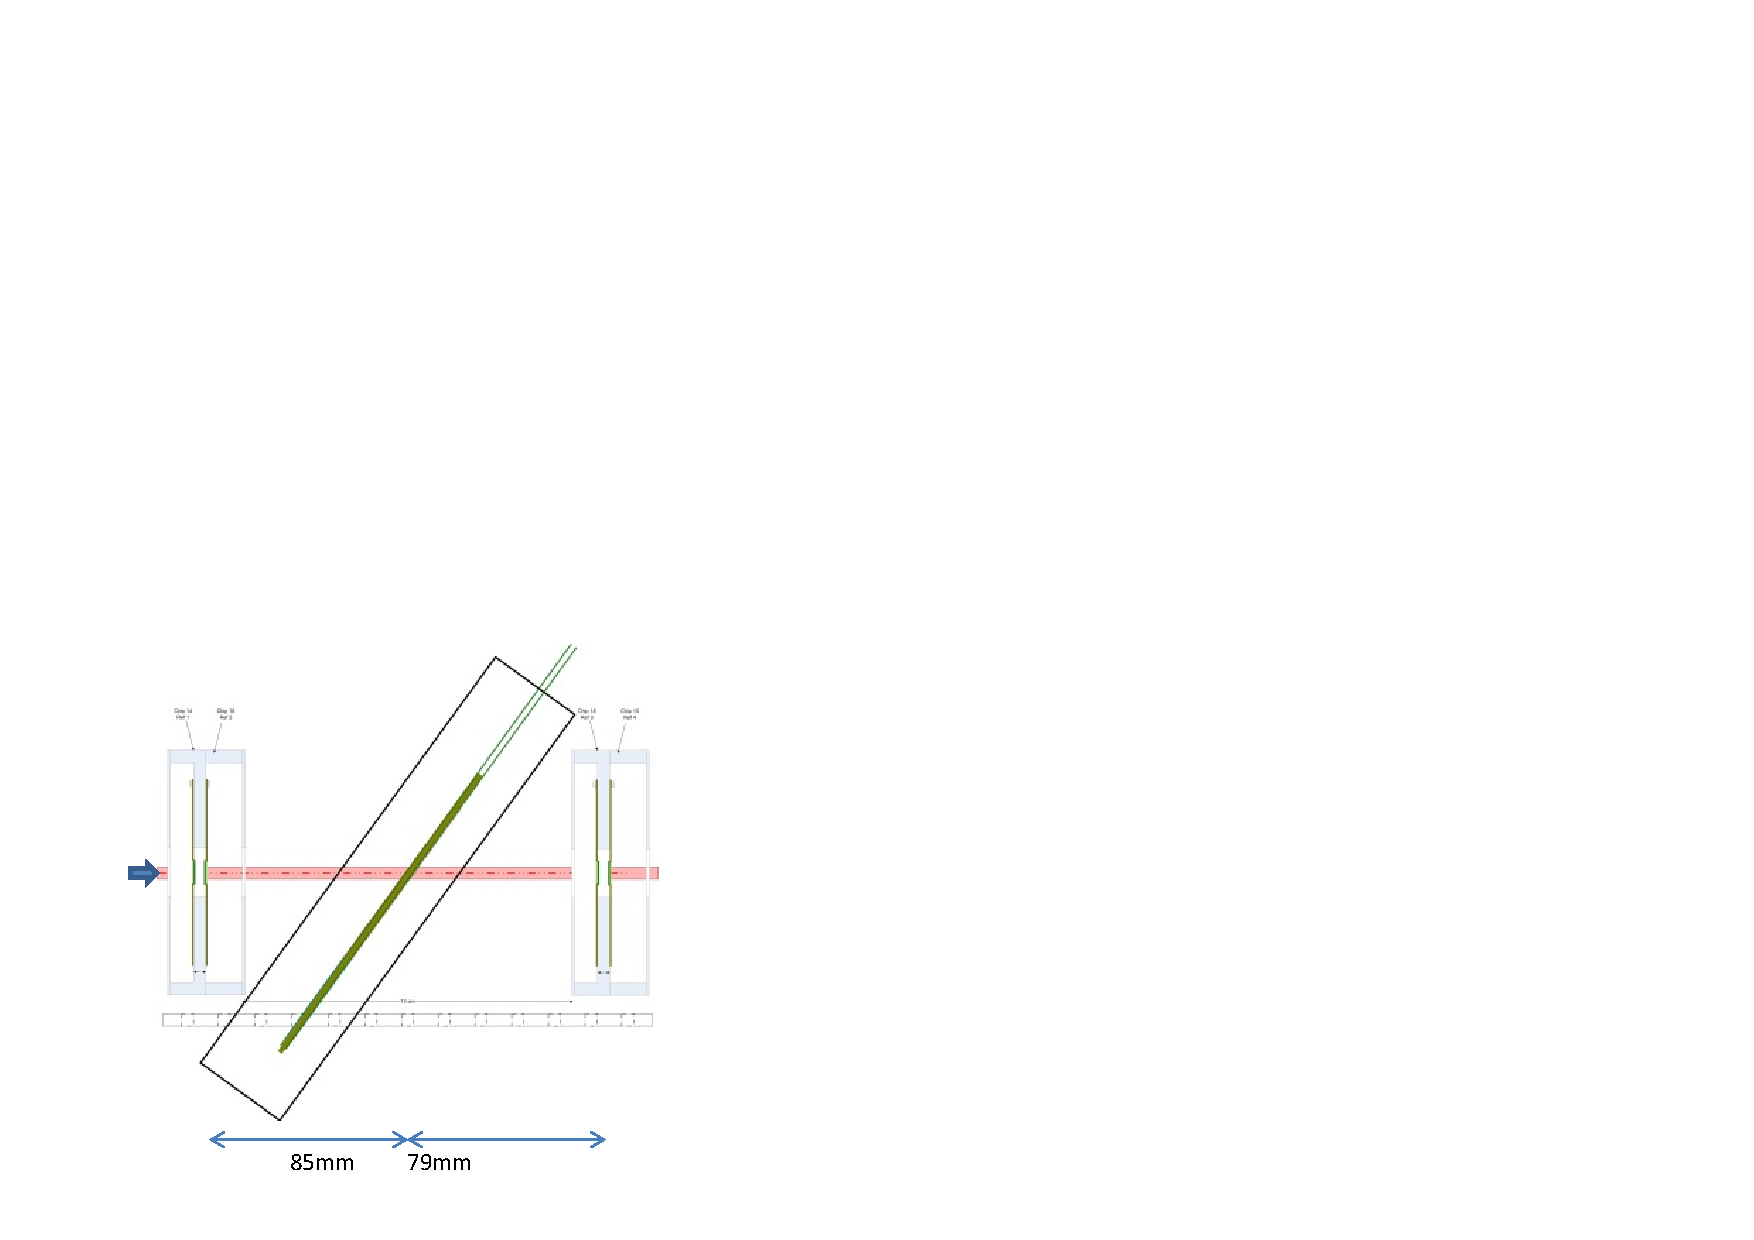
\includegraphics[width = 4cm,height = 4.1cm]{Pictures/tb_cern_11_sketch_tilted.pdf}

          \vspace{-0.2cm}
          \footnotesize{\textbf{Module tilted (between 28\degres and 40\degres).}}
        \end{center}
      \end{column}

      \begin{column}{4cm}
        \begin{center}
          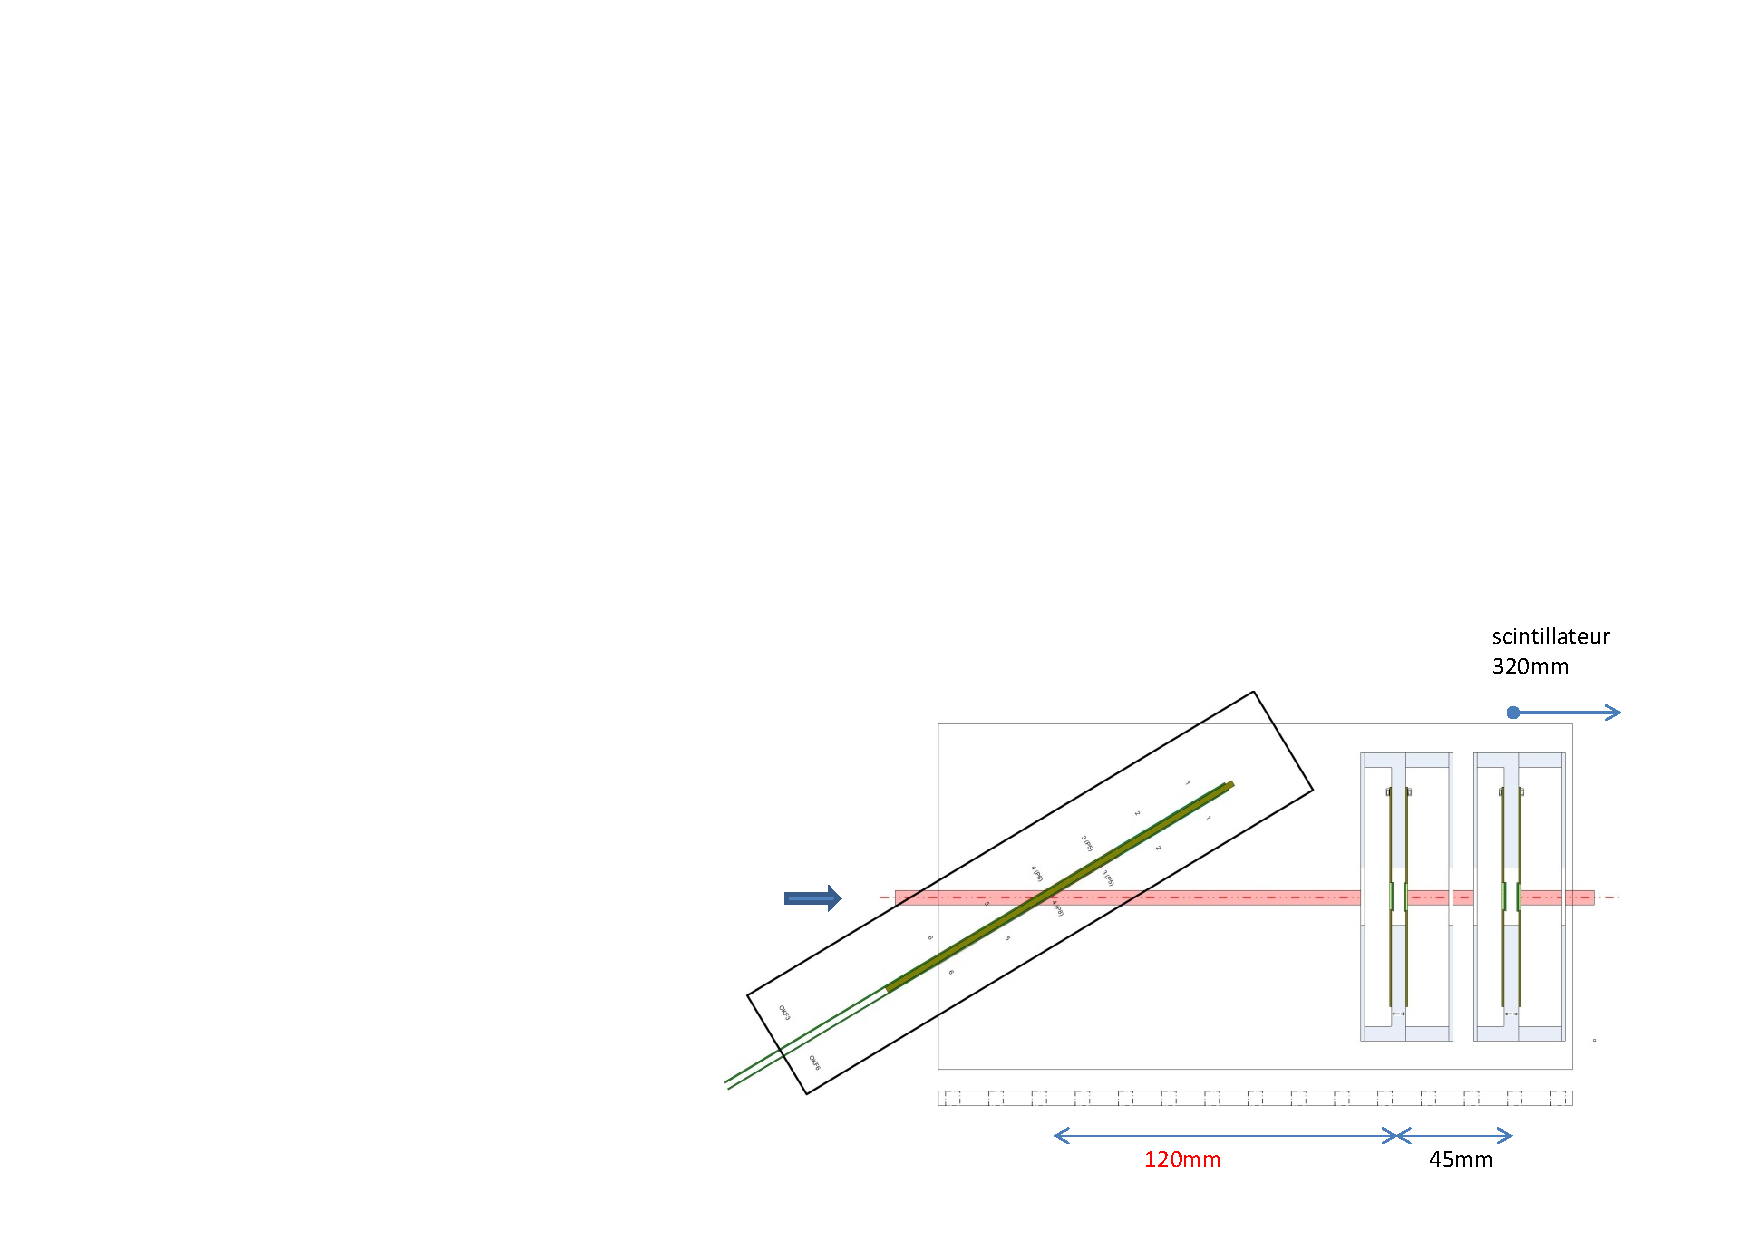
\includegraphics[width = 4cm,height = 4.0cm]{Pictures/tb_cern_11_sketch_tilted120mm.pdf}

          \footnotesize{Module tilted ($\simeq$ 60\degres).}
        \end{center}
      \end{column}
    \end{columns}

    \vspace{0.1cm}
    \footnotesize{$\Rightarrow$ Study track-hit residual and the distribution of this residual as a function of the relative position of the beam on the sensor.

    \vspace{0.1cm}
    \centering{\textbf{Analysis performed with TAF (TAPI Analysis Framework). }}}
    %\grille
\end{frame}

%-------------------------------
%                           RUN Normal incidence
%-------------------------------
\begin{frame}
  \frametitle{Module perpendicular to the beam}

  \begin{center}
    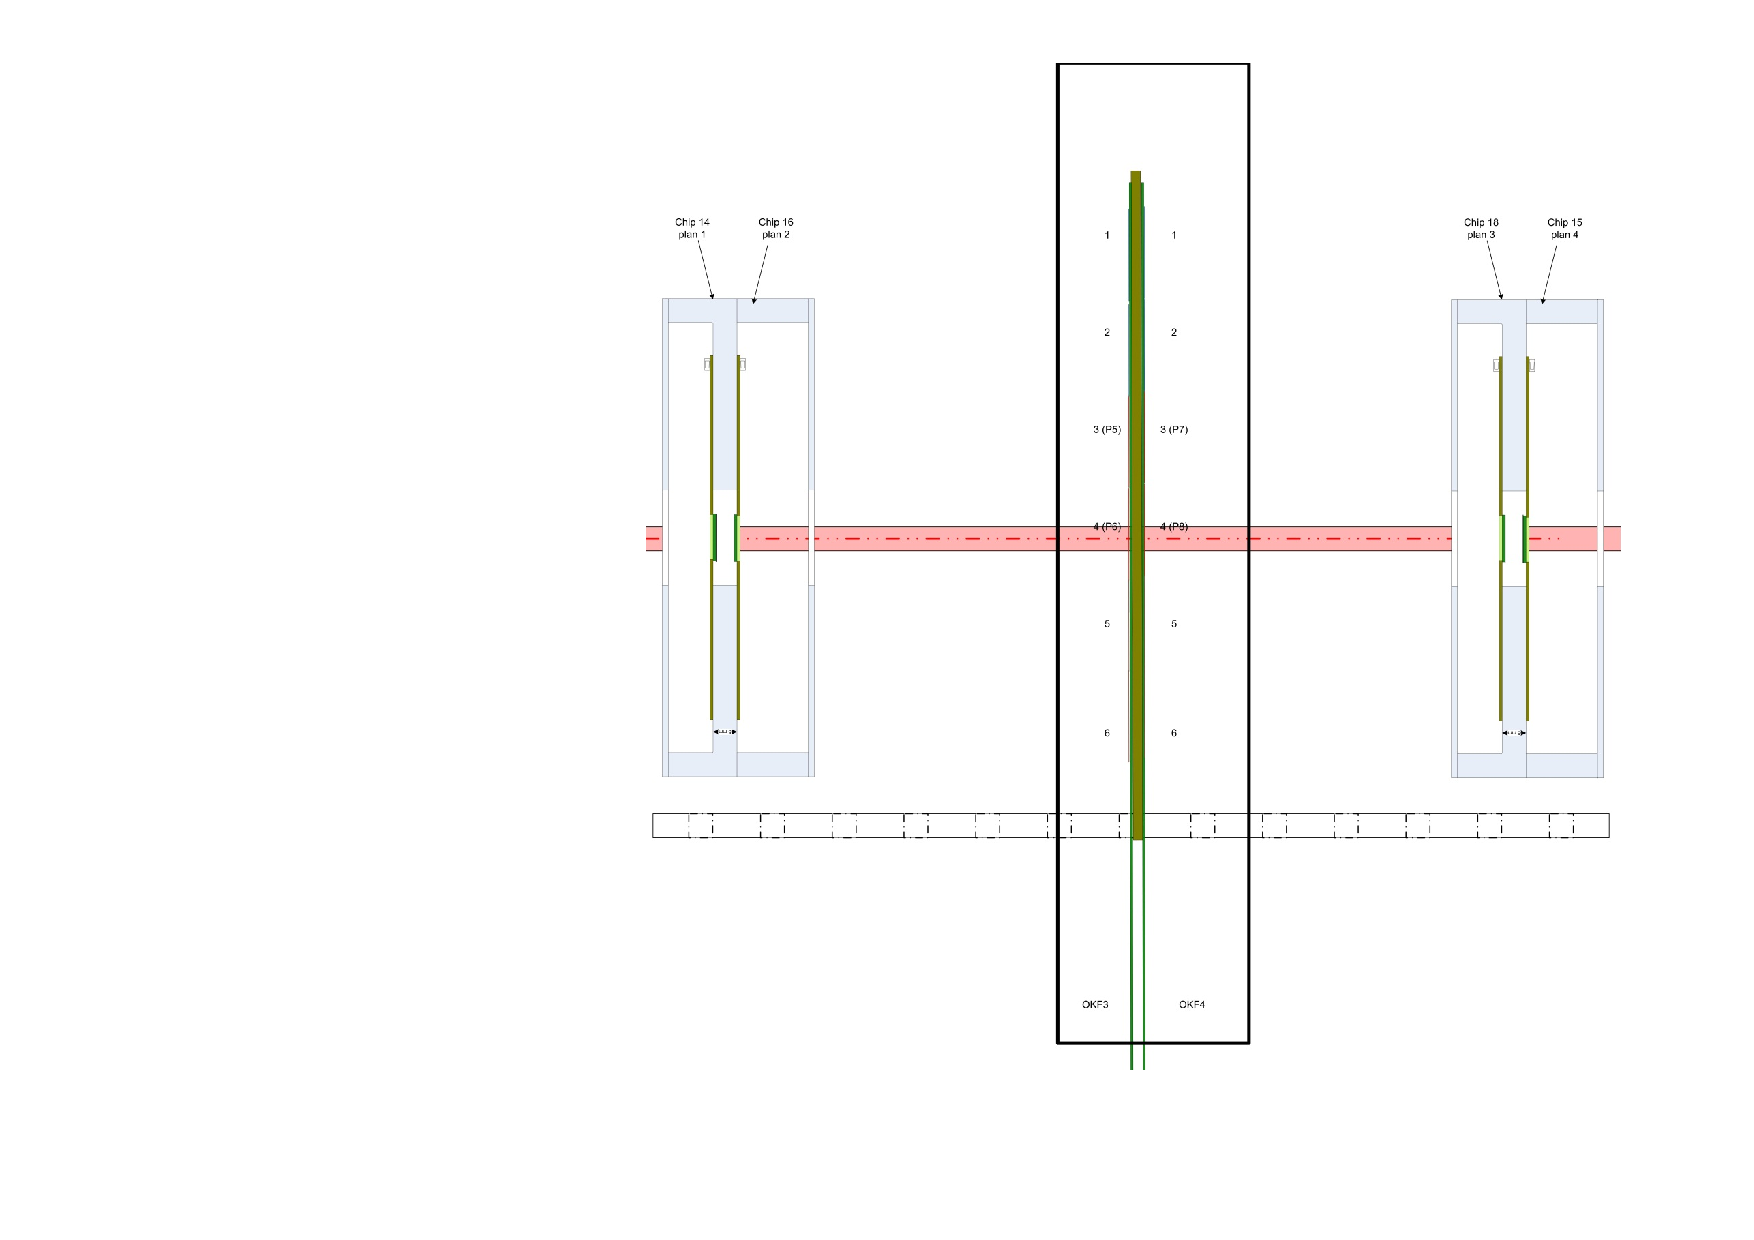
\includegraphics[width = 0.7\textwidth, height = 5cm]{Pictures/tb_cern_11_sketch_normal.pdf}
  \end{center}
\end{frame}

\begin{frame}
  \frametitle{Module perpendicular to the beam}

  \vspace{-0.2cm}
  \centering{Threshold 6 $\sigma$, air flow speed < 5m/s and 1.8M events.}

  \vspace{-0.2cm}
  \begin{center}
    \begin{columns}[t]
      \begin{column}{4cm}
        \centering
        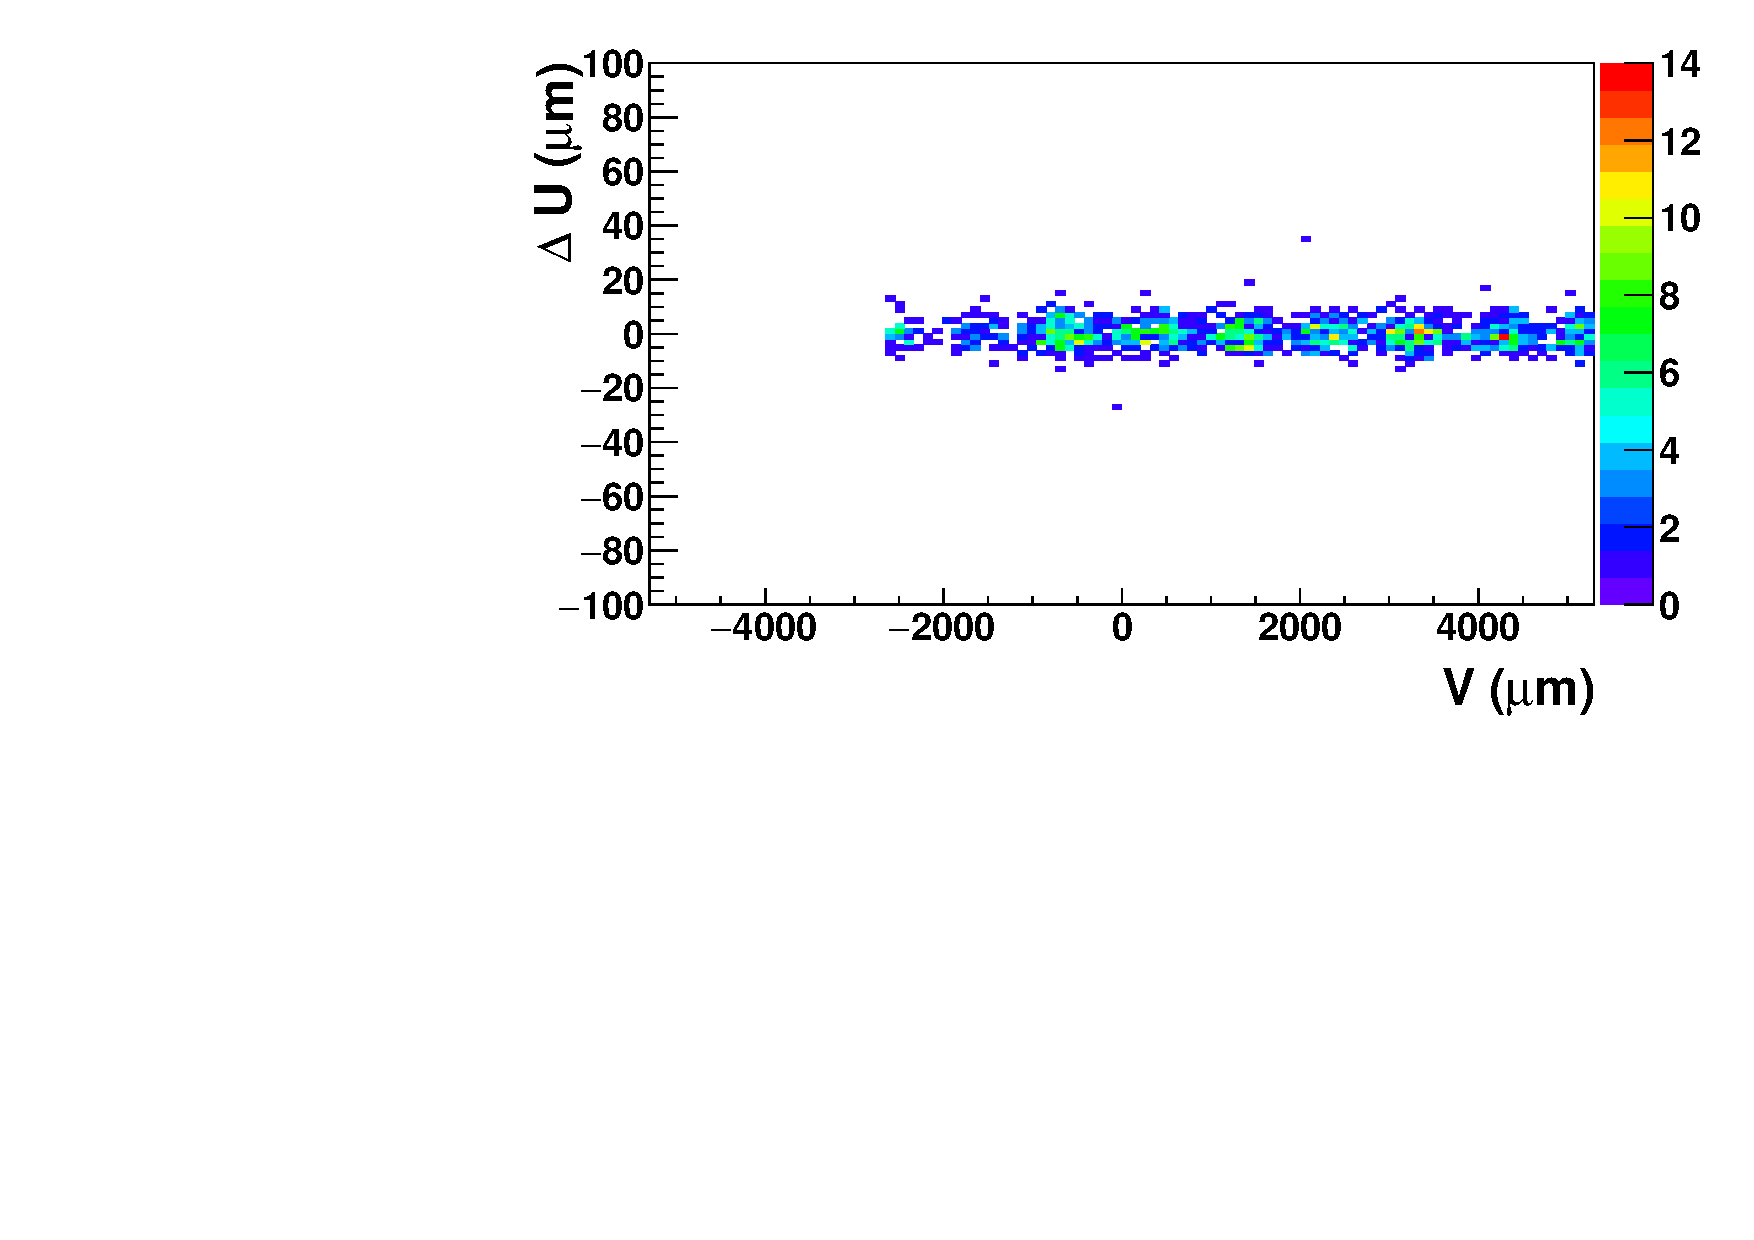
\includegraphics[width = 4cm, height = 1.8cm]{Pictures/deltaUV_6_normal_incidence.pdf}
        \
        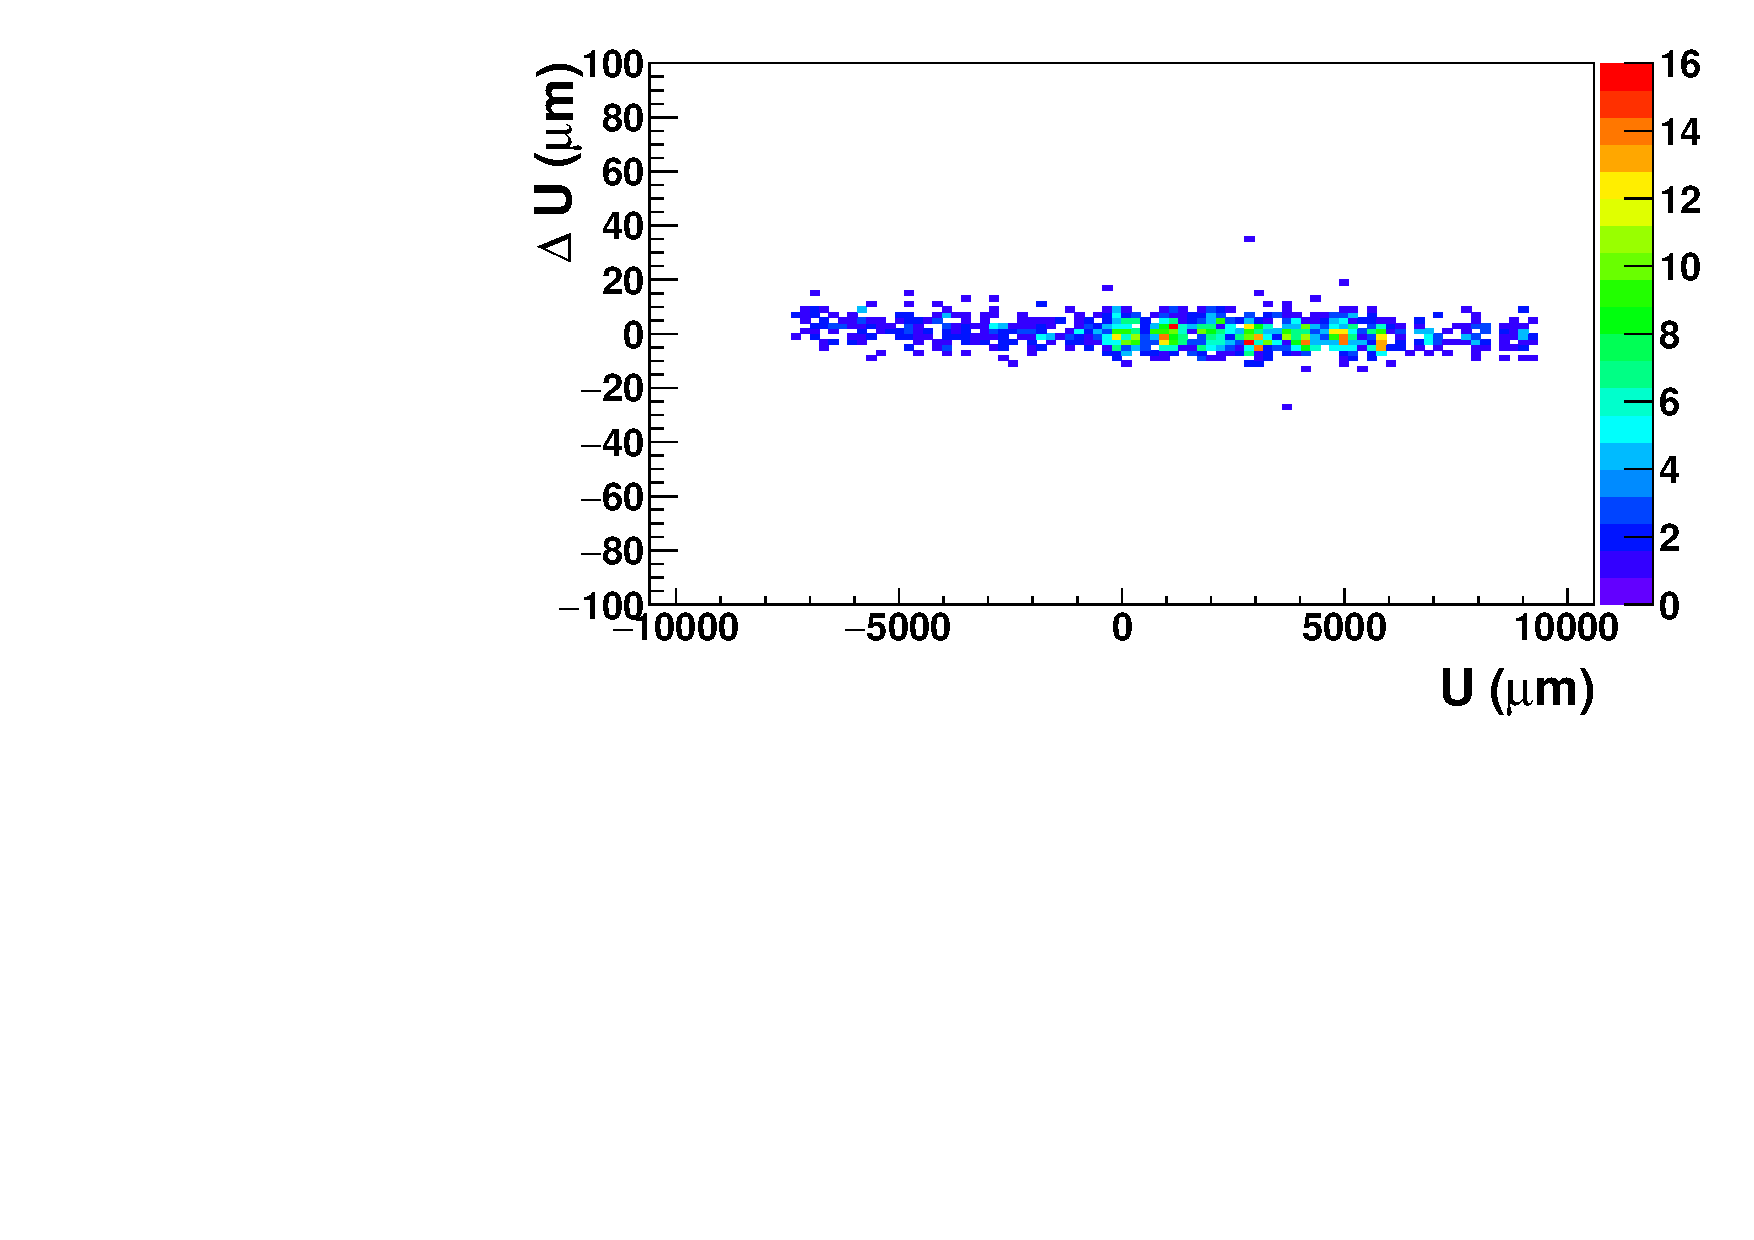
\includegraphics[width = 4cm, height = 1.8cm]{Pictures/deltaUU_6_normal_incidence.pdf}
        \
        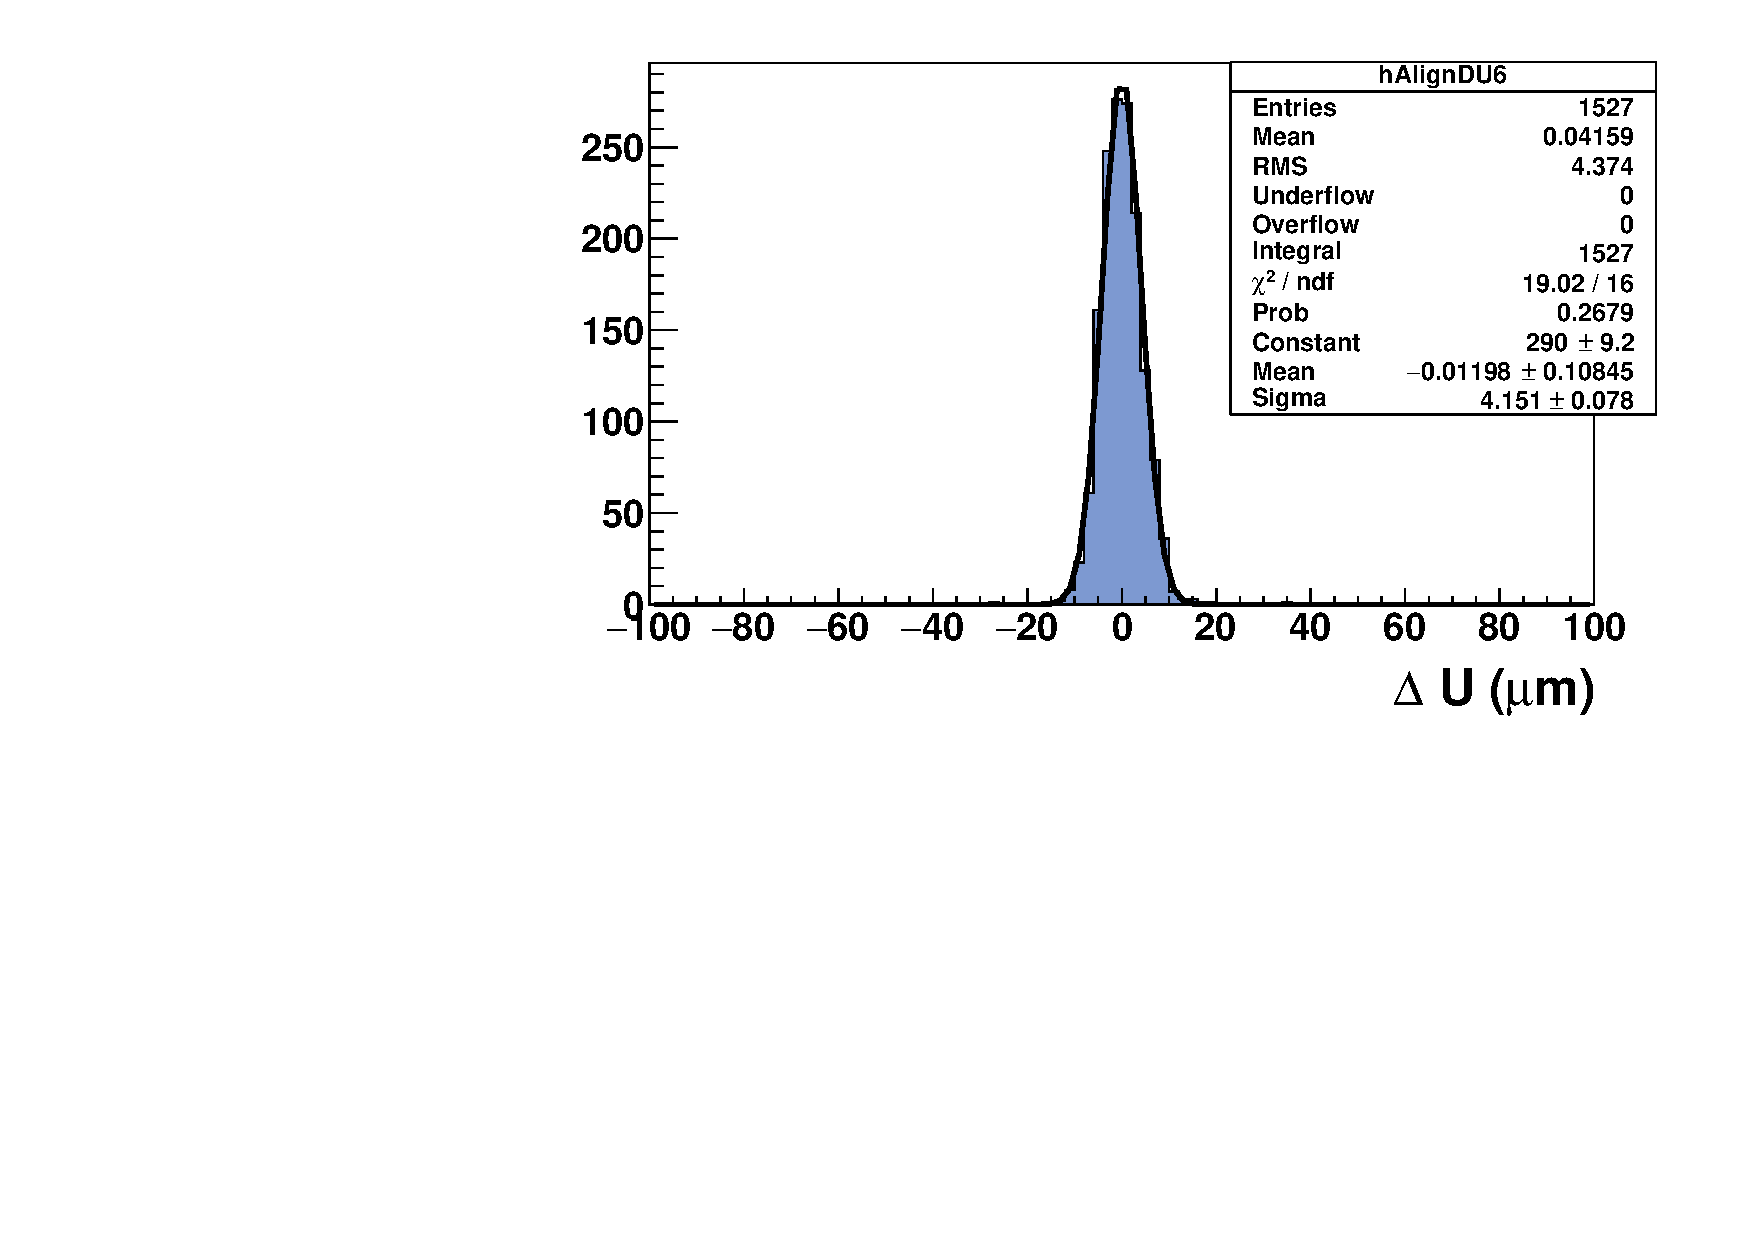
\includegraphics[width = 4cm, height = 1.8cm]{Pictures/deltaU_6_normal_incidence.pdf}
      \end{column}
      \begin{column}{4cm}
        \centering
        \includegraphics[width = 4cm, height = 1.8cm]{Pictures/deltaVU_6_normal_incidence.pdf}
        \
        \includegraphics[width = 4cm, height = 1.8cm]{Pictures/deltaVV_6_normal_incidence.pdf}
        \
        \includegraphics[width = 4cm, height = 1.8cm]{Pictures/deltaV_6_normal_incidence.pdf}
      \end{column}
    \end{columns}
      %\includegraphics[width = 10cm]{Pictures/RsAlign_226056_pl6.png}
  \end{center}

  \vspace{-0.35cm}
  \centering{Spatial residual obtained after alignment:}

  \centering{$ \sigma_U \simeq 4.2~\mu\text{m and } \sigma_V \simeq 4.1~\mu\text{m}$}
\end{frame}

%-------------------------------
%                           RUN Tilt of 36 degres
%-------------------------------
\begin{frame}
  \frametitle{Module tilted in one direction (36\degres)}

  \begin{center}
    \includegraphics[width = 0.6\textwidth]{Pictures/tb_cern_11_sketch_tilted.pdf}
  \end{center}
\end{frame}
\begin{frame}
  \frametitle{Module tilted in one direction (w.r.t. to the beam axis)}

  \vspace{-0.2cm}
  \centering{Threshold 6 $\sigma$, air flow speed <  5m/s, 720k events and 36\degres tilt.}

  \vspace{-0.2cm}
  \begin{center}
    \begin{columns}[t]
      \begin{column}{4cm}
        \centering
        \includegraphics[width = 4cm, height = 1.8cm]{Pictures/deltaUV_8_deformed.pdf}
        \
        \includegraphics[width = 4cm, height = 1.8cm]{Pictures/deltaUU_8_deformed.png}
        \
        \includegraphics[width = 4cm, height = 1.8cm]{Pictures/deltaU_8_deformed.png}
      \end{column}
      \begin{column}{4cm}
        \centering
        \includegraphics[width = 4cm, height = 1.8cm]{Pictures/deltaVU_8_deformed.pdf}
        \
        \includegraphics[width = 4cm, height = 1.8cm]{Pictures/deltaVV_8_deformed.png}
        \
        \includegraphics[width = 4cm, height = 1.8cm]{Pictures/deltaV_8_deformed.png}
      \end{column}
    \end{columns}
      %\includegraphics[width = 10cm]{Pictures/RsAlign_226057_pl6.png}
  \end{center}

  \vspace{-0.35cm}
  \centering{Spatial residual obtained after alignment: }

  \centering{$ \sigma_U \simeq 6.8~\mu\text{m and } \sigma_V \simeq 4.0~\mu\text{m}$}

\end{frame}

%-------------------------------
%                           Origin of deviations
%-------------------------------
  \subsection{Origin of deviations and how to take them into account}
  \begin{frame}
    \frametitle{Origin of deviations}

    \vspace{-0.2cm}
    \begin{block}{Consequence of the ladder's characteristics}
      \begin{itemize}
        \item Use of ultra-thin (50 $\mu\text{m}$) and precise sensors (spatial resolution less than $4~\mu\text{m}$)
        \item Mechanical constraints induce permanent deformations ($\simeq 100~\mu\text{m}$) which can not be flattened during the ladder assembly
      \end{itemize}
    \end{block}

    %\vspace{-0.2cm}
    %\centering{Metrology of the module's surface (performed at Bristol)}

    %\vspace{-0.3cm}
    %\begin{columns}[c]
    %  \begin{column}{6cm}
    %    \begin{center}
    %      \includegraphics[width = 5.7cm]{Pictures/SideAPlumeLadder2010_M20.png}
    %    \end{center}
    %  \end{column}

    %  \begin{column}{6cm}
    %    \begin{center}
    %      \includegraphics[width = 6cm]{Pictures/SideBPlumeLadder2010_M20.png}
    %    \end{center}
    %  \end{column}
    %\end{columns}

  \end{frame}

  \begin{frame}
    \frametitle{Origin of the deviations}
    
    \begin{block}{Artefacts from the modelling of our sensors during the analysis}
      \begin{itemize}
        \item Sensors modeled as completely flat planes
        \item The track extrapolation is sensitive to the exact position of the hit on the plane and the angle of incidence
      \end{itemize}
    \end{block}

    \begin{columns}[c]
      \begin{column}{5cm}
        \vspace{-0.2cm}
        \begin{center}
          \includegraphics[width = 4.8cm]{Pictures/origin_deformation.png}
        \end{center}
      \end{column}

      \begin{column}{5cm}
        \begin{alertblock}{Deviations of the residual}
          \[ \delta W \ = \ \frac{\delta U}{\tan \theta}\]
        \end{alertblock}
      \end{column}
    \end{columns}

  \end{frame}

  %-------------------------------
  %                           How to take into account shape
  %-------------------------------
  \begin{frame}
    \frametitle{How to describe deviations from the flat plane?}

    \vspace{-0.3cm}
    \begin{block}{arXiv:1403.2286 [physics.ins-det] CMS paper}
      \begin{itemize}
        \item Sensor shape parametrised as a sum of products of modified Legendre polynomials:
      \end{itemize}
      \vspace{-0.2cm}
      \[
        \begin{array}{rl}
            w(u_r,v_r) &= w \\ 
                       &+ w_{10} \cdot u_r + w_{01} \cdot v_r \\ 
                       &+ w_{20} \cdot (u_r^2-1/3) + w_{11} \cdot (u_r \cdot v_r) + w_{02} \cdot (v_r^2 - 1/3) \\
        \end{array}
      \]
      \vspace{-0.5cm}
      \begin{itemize}
        \item In our case, we used Legendre polynomials of the $11^{th}$ order only in the direction of the deformation. 
      \end{itemize}
    \end{block}

    \vspace{-0.3cm}
    \begin{center}
      \includegraphics[width = 10.5cm]{Pictures/lagrangianPlynomials.png}
    \end{center} 

  \end{frame}

  %-------------------------------
  %                           Parametrization of the deformation
  %-------------------------------
  \begin{frame}
    \frametitle{Deformation's parametrisation for 36\degres}

    \centering{Possibility to parametrise the deformation with Legendre polynomials of the $11^{th}$ order .} 

    \begin{center}
      \includegraphics[width = 0.8\textwidth]{Pictures/profileFitted_pl8.png}
    \end{center}

    \vspace{-0.8cm}
    \[ \delta W \ = \ \frac{\delta U}{\tan \theta}\]
    %\grille

    \begin{tikzpicture}[overlay,remember picture, red, shift={(current page.south west)}]
      \begin{scope}
        \draw[line width = 2pt,-latex] (8.1,4.05) ellipse (1.2cm and 1.0cm);
      \end{scope}
    \end{tikzpicture}

  \end{frame}

  \subsection{Results on the correction of deviations}
  \begin{frame}
    \frametitle{Summary before/after correction at 36\degres}

    \vspace{-0.35cm}
    \begin{columns}[c]
      \begin{column}{5cm}
        \begin{block}{Before correction}
          \begin{center}
            \includegraphics[width = 0.99\textwidth]{Pictures/deltaUU_8_deformed.png}
            \
            \includegraphics[width = 0.99\textwidth]{Pictures/deltaU_8_deformed.png}
          \end{center}

          \vspace{-0.54cm}
          \centering{\footnotesize{$ \sigma_{u} = 6.8~\mu m$}}
        \end{block}
      \end{column}

      \begin{column}{5cm}
        \begin{block}{After correction}
          \begin{center}
            \includegraphics[width = 1.01\textwidth]{Pictures/deltaUU_8_corrected1.png}
          \
          \includegraphics[width = 1.01\textwidth]{Pictures/deltaU_8_corrected1.png}
          \end{center}

          \vspace{-0.52cm}
          \centering{\footnotesize{$ \sigma_{u} = 5.9~\mu m $}}
        \end{block}
      \end{column}
    \end{columns}

  \end{frame}

  \begin{frame}
    \frametitle{Summary of correction for different angles and same planes}

    \vspace{-0.28cm}
    \begin{block}{Spatial residuals}
      \begin{center}
        \begin{tabular}{c K{1cm} c c K{2cm}}
          \hline %----------------------------------------------------------------------------------------------------------------
          Side &  Tilted angle ($^{\circ}$)  &   $\sigma_{U}^{Def}~(\mu m$) &   $\sigma_{U}^{Cor}~(\mu m$) & Improvement \\
          \hline %----------------------------------------------------------------------------------------------------------------
          \hline %----------------------------------------------------------------------------------------------------------------
          Front &      28       & $ 9.0 \ \pm \ 0.1 $ & $ 4.9 \ \pm \ 0.1 $ &    $46.6 \ \%$  \tabularnewline
          Back  &      28       & $ 5.7 \ \pm \ 0.1 $ & $ 4.7 \ \pm \ 0.1 $ &    $17.5 \ \%$  \tabularnewline
          \hline %----------------------------------------------------------------------------------------------------------------
          Front &      36       & $ 14.1 \ \pm \ 0.1 $ & $ 6.1 \ \pm \ 0.1 $ &    $56.0 \ \%$ \tabularnewline
          Back  &      36       & $ 6.8 \ \pm \ 0.1 $ & $ 5.9 \ \pm \ 0.1 $ &    $13.2 \ \%$  \tabularnewline
          \hline %----------------------------------------------------------------------------------------------------------------
          Front &      60       & $ 41.2 \ \pm \ 0.15$ & $25.8 \ \pm \ 0.2$  &    $37.4 \ \%$ \tabularnewline
          Back  &      60       & $ 23.3 \ \pm \ 0.13$ & $21.7 \ \pm \ 0.1$  &    $6.8 \ \%$  \tabularnewline
          \hline %----------------------------------------------------------------------------------------------------------------
        \end{tabular}
      \end{center}
      \vspace{-0.35cm}
      \centering{$\sigma_{tel} = 2.2 \mu m$ for 36\degres and $\sigma_{tel} = 18.8 \mu m$ for 60\degres.}
    \end{block}

  \end{frame}

\section{Material budget measurement}
\begin{frame}
  \frametitle{Outlines}
  \begin{minipage}{\textwidth}
  \footnotesize
    \tableofcontents[currentsection,hideothersubsections, 
    sectionstyle=show/shaded]
  \end{minipage}
\end{frame}

  \subsection{Motivation}

  \begin{frame}
    \frametitle{Multiple scattering}
    
    \vspace{-0.4cm} 
    \begin{block}{Charged particles traveling through matter}
      \vspace{-0.3cm}
      \begin{columns}[c]
        \begin{column}{5cm}
          \footnotesize
          \begin{itemize}
            \item Lose energy via inelastic collisions with atomic electrons
            \item Deflection by many small angles (Coulomb scattering from nuclei)
            \item Standard deviation of the scattering angle distribution described by Highland formula
          \end{itemize}
          \vspace{-0.1cm}
          \centering
            \[ \theta_0 = \frac{13.6 (MeV)}{p}\left( \frac{x}{X_0}\right)^{0.555}\]
        \end{column}
        \begin{column}{6cm}
          \centering
          \includegraphics[width = 5cm]{Pictures/multiple_scattering.jpg}
        \end{column}
      \end{columns}
    \end{block}

    \vspace{-0.3cm}
    \begin{block}{Motivation of measuring the material budget}
      \footnotesize
      \begin{itemize}
        \item Key parameter for tracking algorithm: has to take into account multiple scattering and energy degradation
        \item Compare material budget prediction to its result after construction
        \item Goal: mapping in $uv$ of X$_0$
      \end{itemize}
    \end{block}
  \end{frame} 
  
  \subsection{Test beam @ DESY}

  \begin{frame}
    \frametitle{Test beam @ DESY with 5 GeV $e^-$ (April 2016)}
    
    \begin{columns}[c]
      \begin{column}{5cm}
        \begin{center}
          \includegraphics[width = \textwidth]{Pictures/testBeam.png}
        \end{center}
      \end{column}
      \begin{column}{5cm}
        \begin{itemize}
          \item Test Beam 21
          \item Reference plane: 4 EUDET telescope planes
          \item Goal: material budget measurement
        \end{itemize}
      \end{column}
    \end{columns}
  \end{frame}

  \subsection{Theoretical estimation}
  
 
  \begin{frame}
    \frametitle{Kink angle measurement}

    \begin{center}
      \includegraphics[width = 0.7\textwidth]{Pictures/kinkAngleTB.png}
    \end{center}
  \end{frame}

  \subsection{Results}

  \begin{frame}
    \frametitle{Kink angle measurement at 4 GeV}

      \begin{center}
        \includegraphics[width = 0.7\textwidth]{Pictures/kinkAngle4GeV.png}
      \end{center}
      \vspace{-0.2cm}
      \begin{block}{Determination of projected scattering angle $\theta_0$}
        \centering{$\theta_0 = \sqrt{sigma^2 - F}$}
        \begin{itemize}
          \item $sigma$ = sigma of the kink angle distribution fit
          \item $F$ = Offset parameter from the GBL track fitting algorithm
        \end{itemize}
      \end{block}
  \end{frame}

  \begin{frame}
    \frametitle{Material budget}

    \vspace{-0.3cm}
    \begin{center}
      \includegraphics[width = 0.8\textwidth]{Pictures/theta0VsP_2-4GeV.png}
    \end{center}

    \vspace{-0.4cm}
    \begin{block}{Measurement}
      \begin{center}
      Highland formula: $\theta_0 = \frac{13.6 (MeV)}{p}\left( \frac{x}{X_0}\right)^{0.555}$
      \ 
       $\frac{\text{x}}{\text{X}_0}\left|_{measured} \simeq 0.47 \pm 0.02~\%~\text{X}_0 \right.$
      \end{center}
    \end{block}

  \end{frame}

   \begin{frame}
    \frametitle{Estimation of the radiation length}

    \begin{columns}[c]
      \begin{column}{4cm}
        \centering
        \includegraphics[width = 0.9\textwidth]{Pictures/X0.pdf}
        
      \end{column}
      \begin{column}{5cm}
        \centering
        \includegraphics[width = 1.1\textwidth]{Pictures/flexPCB-2009.jpg}

        %\includegraphics[width = \textwidth]{Pictures/X02.pdf}
        %\begin{block}{Beam passes through}
        %  %\begin{itemize}
        %  %  \item $2 \times$ Mi-26 (thinned down to $\sim 50~\mu$m): $0.053~\%$ X$_0$
        %  %  \item $4 \times$ glue layers: $\sim 0.01~\%$ X$_0$
        %  %  \item $1 \times$ SiC foam: $\sim 0.184~\%$ X$_0$
        %  %  \item $2 \times$ flex-cable: $\sim 0.084 - 0.092~\%$ X$_0$
        %  %  %\item $2 \times$ flex cable: $\sim 0.084~-~0.092~\%$ X$_0$
        %  %\end{itemize}
        %  %$\Rightarrow \frac{\text{x}}{\text{X}_0} \simeq 0.498~-~0.515~\%~\text{X}_0$
        %\end{block}
      \end{column}
    \end{columns}

    \begin{block}{Total material budget}
      \centering 
      Depends on flex-cable fill factor (25~\% or 30~\%)
      $\Rightarrow \frac{\text{x}}{\text{X}_0} \simeq 0.498~-~0.515~\%~\text{X}_0$
      \\
      \only<2>{$\frac{\text{x}}{\text{X}_0}\left|_{measured} \simeq 0.47 \pm 0.02~\%~\text{X}_0 \right.$}
    \end{block}
  \end{frame}


  \begin{frame}
    \frametitle{Lower estimation of X$_0$}

    \begin{columns}[c]
      \begin{column}{5cm}
        \begin{center}
          \includegraphics[width = 1.2\textwidth]{Pictures/SignalReconstructionMi26.png}
        \end{center}
      \end{column}
      
      \begin{column}{4.5cm}
        \begin{block}{Possible explanation}
          \begin{itemize}
            \item During analysis, hit position is located in middle of the epitaxial layer
            \item Missing $6~\mu$m of the electronic layers and $7~\mu$m of epitaxial layer
            \item For 2 sensors $\Rightarrow$ $ \sim 0.028~\%$ X$_0$ not included in the calculation
          \end{itemize}
        \end{block}
      \end{column}
    \end{columns}

  \end{frame}

    
\section{Conclusion and outlook} 
\begin{frame}
  \frametitle{Outlines}
  \begin{minipage}{\textwidth}
  \footnotesize
    \tableofcontents[currentsection,hideothersubsections, 
    sectionstyle=show/shaded]
  \end{minipage}
\end{frame}

\begin{frame}
  \frametitle{Conclusion 1/2}

  \begin{block}{Context}
    \begin{itemize}
      \item The ILC is the next colliding machine to study precisely EWSB (and other physics scenarios)
      \item The Higgs boson will be more precisely characterised
      \item Physics performance to achieve requires a new R\&D detector development 
    \end{itemize}
  \end{block}

  \begin{block}{Higgs boson study}
    To achieve a precision of $\sim 1~\%$ in the Higgs boson branching ratio measurement a simple sequential cuts is not the best option
  \end{block}

  \vspace{-0.23cm}

\end{frame}

\begin{frame}
  \frametitle{Conclusion 2/2}

    \begin{block}{PLUME development}
    PLUME is the first double-sided layers developed according to the ILD requirements
    \begin{itemize}
      \item Impact of the mechanical structure
      \begin{itemize}
        \item Mechanical structure induces permanent deformations which have an impact on ladder's performance
        \item Algorithm based on Legendre polynomials is able to reduce the impact of these deformations on ladder's performance
      \end{itemize}
      \item Material budget
      \begin{itemize}
        \item Material budget is predicted from construction
        \item Measurement of this material budget for PLUME-1 gives:
      \end{itemize}
    \end{itemize}
    \begin{center}
      $\frac{\text{x}}{\text{X}_0}\left|_{measured} \simeq 0.47 \pm 0.02~\%~\text{X}_0 \right.$

      $\frac{\text{x}}{\text{X}_0}\left|_{estimated} \simeq 0.498~-~0.515~\%~\text{X}_0 \right.$
     \end{center}
  \end{block}
\end{frame}

\begin{frame}
  \frametitle{Outlook 1/2}

  \vspace{-0.25cm}
  \begin{block}{Test beam 2016}
    \begin{itemize}
      \item Mapping in $uv$ of X$_0$
      \item Study ladder performance at low energy
    \end{itemize}
  \end{block}

  \vspace{-0.15cm}
  \begin{block}{PLUME-2}
    New prototype with a material budget of $0.35~\%$ X$_0$ has been built and tested in the laboratory but not yet in real conditions
  \end{block}

  \vspace{-0.15cm}
  \begin{block}{Next PLUME ladder}
    \begin{itemize}
      \item Higher constraint on material budget ($0.3~\%$ X$_0$)
      \item Enriching double-sided layer concept with sensors having different characteristics (fast integration time VS good spatial resolution)
      \item Adapt sensor technology and cooling system to the \hyperlink{power-pulsing}{ILC beam structure}
    \end{itemize}
  \end{block}


\end{frame}

\begin{frame}
  \frametitle{Outlook 2/2}

    \begin{block}{BEAST project}
    PLUME-2 will be used in the BEAST project at SuperKEKB
    \vspace{-0.2cm}
    \begin{center}
      \includegraphics[width = 0.7\textwidth]{Pictures/plumeInTableDesySetup.jpg}
    \end{center}
  \end{block}
\end{frame}

\begin{frame}
  \begin{center}
    \huge
    \textbf{Thanks for your attention !!!}
  \end{center}
\end{frame}
%-------------------------------
%   BACK-UP
%-------------------------------

  \appendix
%-------------------------------
%   STOP FRAME COUNTING
%-------------------------------
  \newcounter{lastframe}
  \setcounter{lastframe}{\insertframenumber}
  %\setbeamertemplate{footline}[default]  % vide

%-------------------------------
%   BACK-UP: HIGGS POTENTIAL
%-------------------------------
  \begin{frame}[plain]
    \frametitle{Higgs boson potential}

    \begin{center}
      \includegraphics[width = 0.8\textwidth]{Pictures/higgsPotential.png}
    \end{center}
  \end{frame}

%-------------------------------
%   BACK-UP: HIGGS POTENTIAL
%-------------------------------
  \begin{frame}[plain]
    \frametitle{Higgs boson physics at the ILC}

    \begin{itemize}
      \item Same measurements as LHC: couplings, mass and spin
      \item Model independent measurement: no dependence on theory
      \item Total Higgs width
      \item $H \rightarrow c\overline{c}/gg$
      \item Higgs self couplings
    \end{itemize}
  \end{frame}

  \begin{frame}[plain]
    \frametitle{Higgs branching ratio}

    \begin{center}
      \includegraphics[width = 5cm]{Pictures/higgsbr.jpg}
    \end{center}
  \end{frame}

%-------------------------------
%   BACK-UP: Ladder assembly
%-------------------------------
  \begin{frame}[plain]
    \frametitle{Ladder assembly}

    \begin{center}
      \uncover<1->{\includegraphics[width = 0.8\textwidth]{Pictures/plumeLadderAssembly_step1.png}}
      \
      \uncover<2>{\includegraphics[width = 0.8\textwidth]{Pictures/plumeLadderAssembly_step2.png}}
    \end{center}

  \end{frame}

%-------------------------------
%   BACK-UP: PLUME history
%-------------------------------
  \begin{frame}[plain]
    \frametitle{PLUME history}

    \begin{columns}[t]
      \begin{column}{5cm}
        \centering
        PLUME-V0 (2009)

        \includegraphics[width = \textwidth]{Pictures/plume_ladder2009_1.jpg}
      \end{column}
      \begin{column}{5cm}
        \centering
        PLUME-V1 (2010)

        \includegraphics[width = \textwidth]{Pictures/plume_ladder2010_frontView.jpg}
      \end{column}
    \end{columns}
  \end{frame}

%-------------------------------
%   BACK-UP: FOAM
%-------------------------------
\begin{frame}[plain]
  \frametitle{Silicon-Carbide foam support structure}

  \vspace{-0.6cm}
  \begin{columns}[t]

    \begin{column}{4cm}
      \begin{center}
        \includegraphics[width = 4cm]{Pictures/foam1.png}
      \end{center}
    \end{column}

    \begin{column}{4cm}
      \begin{center}
        \includegraphics[width = 4cm]{Pictures/foam2.png}
      \end{center}
    \end{column}

    \begin{column}{4cm}
      \vspace{-0.2cm}
      \begin{center}
        \begin{block}{Properties}
          \begin{itemize}
            \item Open-cell foam
            \item Macroscopically uniform
            \item No tensioning needed
            \item Density: 4 to 8~\% \\ (2-3~\% possible)
            \item Low thermal and electrical conductivity \\ (50 W/m/K)
          \end{itemize}
        \end{block}
      \end{center}
    \end{column}

  \end{columns}

\end{frame}

%-------------------------------
%   BACK-UP: Mi26
%-------------------------------

  \begin{frame}[plain]
    \frametitle{MIMOSA-26 description}

    \begin{center}
      \includegraphics[width = \textwidth]{Pictures/mimosa26_shortDescription.png}
    \end{center}
  \end{frame}

  \begin{frame}[plain]
    \frametitle{MIMOSA-26 architecture}

    \begin{center}
      \includegraphics[width = \textwidth]{Pictures/mi26_architecture.pdf}
    \end{center}
  \end{frame}
%-------------------------------
%   BACK-UP: SUZE
%-------------------------------
  \begin{frame}[plain, label=suze]
    \frametitle{Zero Suppression logic (SUZE)}

    \vspace{-0.4cm}
    \begin{center}
        \includegraphics[width = 7 cm]{Pictures/suze_hitDetection.png}

        \includegraphics[width = 7cm]{Pictures/suze_hit2.png}
    \end{center}

    \vspace{-0.3cm}
    \scriptsize

    SUZE logic split in 3 blocks:
    \begin{itemize}
        \item \textbf{Sparse Data Scan (SDS)} Hit detection per line and data encoding, until 6 states consecutive pixels (1 to 4 pixels) per block of 64 columns;
        \item \textbf{Multiplexing Logic (Mux)} giving up to 9 states;
        \item \textbf{Memory storage} 2 blocks to store the states of the full frame, switching to avoid dead time (during one acquire states of event N, the other one transfer the information of frame N-1).
    \end{itemize}
    %\grille

  \end{frame}

%-------------------------------
%   BACK-UP: Column parallel readout
%-------------------------------

  \begin{frame}[plain]
    \frametitle{Column parallel readout}

    \begin{center}
      \includegraphics[width = 0.8\textwidth]{Pictures/parallelColumnPrinciple_2bis.png}
    \end{center}
  \end{frame}

%-------------------------------
%   BACK-UP: MAPS principle
%-------------------------------

  \begin{frame}[plain]
    \frametitle{MAPS principle}

    \begin{center}
      \includegraphics[width = \textwidth]{Pictures/collectionEfield.png}
    \end{center}
  \end{frame}


  \begin{frame}[plain]
    \frametitle{Young Modulus}

    \begin{center}
      \includegraphics[width = \textwidth]{Pictures/youngModulus_vs_radiationLength-004.jpg}
    \end{center}
  \end{frame}
%-------------------------------
%   BACK-UP: Spatial resolution VS pitch
%-------------------------------

  \begin{frame}[plain]
    \frametitle{Spatial resolution for different pitch (IPHC-Strasbourg)}

    \vspace{-0.3cm}
    \begin{center}
        \includegraphics[width = 10cm]{Pictures/resolution_pitch_10to40_withBinary.png}
    \end{center}
  \end{frame}

%-------------------------------
%   Threshold scan + noise and offset 
%-------------------------------

\begin{frame}[plain]
  \frametitle{Characterization of one sensor}

  \begin{columns}[t]
    \begin{column}{6cm}
      \includegraphics[width = 6cm, height = 4.4cm]{Pictures/transfer_A.png}
      
      \begin{block}{Threshold scan}
        Normalised response of pixels in a sub-matrix (288 discriminators) as a function of threshold applied (mV). 
      \end{block}

    \end{column}

    \begin{column}{6cm}
      \includegraphics[width = 6cm, height = 4.4cm]{Pictures/noise_A.png}

      \begin{block}{Noise performances}
        \footnotesize{
        \begin{itemize}
          \item Temporal noise (derivative of the S-curve): 0.79 mV
          \item Fixed pattern noise (thresholds' dispersion for a mid-point): 0.2 mV
          \item Offset: 0.16 mV
        \end{itemize}
        }
      \end{block}
    \end{column}
  \end{columns}

  \vspace{0.2cm}
  \textbf{$\Rightarrow$ Can now define different thresholds}

  %\grille

  \begin{tikzpicture}[overlay,remember picture, red, shift={(current page.south west)}]
    \begin{scope}
      \draw[line width = 2pt,-latex] (6,6) node[above] {Noise} node[below] {estimation} (5.5,6) -- (6.5,6) ;
    \end{scope}
  \end{tikzpicture}
\end{frame}


  %\begin{frame}
  %  \frametitle{Correction of the deviations between real hits and extrapolated ones}
  %
  %  \vspace{-0.35cm}
  %  \begin{center}
  %    \begin{columns}[t]
  %      \begin{column}{4cm}
  %        \centering
  %        \includegraphics[width = 1.2\textwidth]{Pictures/deltaUV_8_corrected1.png}
  %        \
  %        \includegraphics[width = 1.2\textwidth]{Pictures/deltaUU_8_corrected1.png}
  %      \end{column}
  %      \begin{column}{4cm}
  %        \centering
  %        \includegraphics[width = 1.2\textwidth]{Pictures/deltaVU_8_corrected1.png}
  %        \
  %        \includegraphics[width = 1.2\textwidth]{Pictures/deltaU_8_corrected1.png}
  %      \end{column}
  %    \end{columns}
  %    %\includegraphics[width = 10cm]{Pictures/RsAlign_226057_pl6_corrected.png}
  %  \end{center}
  %
  %  \vspace{-0.35cm}
  %  \centering{Spatial residual obtained after correction: }
  %
  %  \vspace{-0.15cm}
  %  \centering{$\sigma_U \simeq 5.9~\mu\text{m}$ instead of $ \sigma_U \simeq 6.1~\mu\text{m}$}
  %\end{frame}


  \begin{frame}
    \frametitle{Kink angle measurement between 1 and 4 GeV}

    \begin{block}{Fitted kink angle distributions}
      \begin{columns}[c]
        \begin{column}{5cm}
          \centering
          \includegraphics[width = \textwidth]{Pictures/kinkAngle1GeV.png}
          \
          \includegraphics[width = \textwidth]{Pictures/kinkAngle2GeV.png} 
        \end{column} 
        \begin{column}{5cm}
          \centering
          \includegraphics[width = \textwidth]{Pictures/kinkAngle3GeV.png}
          \ 
          \includegraphics[width = \textwidth]{Pictures/kinkAngle4GeV.png}
        \end{column} 
      \end{columns}
    \end{block}
  \end{frame}



%-------------------------------
%   BACK-UP: Physics
%-------------------------------

  \begin{frame}[plain]
    \frametitle{Higgs Strahlung kinematics}

    \[ E_H = \frac{s - \rm{M}_Z^2 + \rm{M}_H^2}{2\sqrt{s}} \]
    \[ E_Z = \frac{s - \rm{M}_H^2 + \rm{M}_Z^2}{2\sqrt{s}} \]
    \[ | \overrightarrow{p_H} | = | \overrightarrow{p_Z} | = \frac{\sqrt{\left[ s - (\rm{M}_H + \rm{M}_Z)^2 \right] \cdot \left[s - (\rm{M}_H - \rm{M}_Z)^2 \right]}}{2\sqrt{s}} \]

    If $\rm{M}_H = 125~\rm{GeV}$, $\rm{M}_Z = 91.2~\rm{GeV}$ and $\sqrt{s} = 350~\rm{GeV}$, then:
    \[ E_H \simeq 185.4~\rm{GeV} \]
    \[ E_Z \simeq 164.6~\rm{GeV} \]
    \[  | \overrightarrow{p_H} | = | \overrightarrow{p_Z} | \simeq 68.5~\rm{GeV}\]

  \end{frame}

%-------------------------------
%   BACK-UP: ILC-ILD
%-------------------------------
  \begin{frame}[plain]
    \frametitle{Detector performances}

    \begin{block}{Vertexing}
      \[ \sigma_{IP} \ = \ 5 \oplus \frac{10}{p\sin^{3/2}\theta} (\mu\rm{m})\]
    \end{block}

    \begin{block}{Tracking}
      \[ \sigma (1/p) \ = \ 2x10^{-5} (\rm{GeV}^{-1})\]
    \end{block}
      
    \begin{block}{Jet ernergy}
      \[\sigma_E / E \ = \ 0.3/\sqrt{\rm{E(GeV)}}\]
    \end{block}

  \end{frame}

%-------------------------------
%   BACK-UP: PFA
%-------------------------------
  \begin{frame}[plain]
    \frametitle{Particle Flow Algorithm}

    \begin{itemize}
      \item Typical jet:
        \begin{itemize}
          \item Charged hadrons $\simeq~60~\%$
          \item Photons $\simeq~30~\%$
          \item Neutral $\simeq~10~\%$
        \end{itemize}
      \item Standard approch
        \begin{itemize}
          \item All jet components energy measured in ECAL/HCAL
          \item $E_{jet} = E_{ECAL} + E_{HCAL}$
        \end{itemize}
      \item Particle flow calorimetry
        \begin{itemize}
          \item Measurement of charged particles in tracker
          \item Measurement of photon in ECAL
          \item Measurement of hadrons in HCAL
          \item $E_{jet} = E_{Track} + E_{\gamma} + E_n$
        \end{itemize}
    \end{itemize}
  \end{frame}

%-------------------------------
%   BACK-UP: WHY LINEAR COLLIDER
%-------------------------------
  \begin{frame}[plain]
    \frametitle{Why a linear collider?}

    \begin{block}{Limitations of $e^+e^-$ colliders}
      \begin{itemize}
        \item Synchroton radiation loss $\sim E^{4}/r$
        \item Synchroton cost: $\sim$ quadratically with energy
        \item Power consumption
      \end{itemize}
    \end{block}
    
    \begin{block}{Avantages of linear colliders}
      \begin{itemize}
        \item Not limited by synchrotron radiation
        \item Cost: $\sim$ linear with energy
        \item Polarisation of both beams
        \item Detectors close to the IP $\Rightarrow$ optimum for $c$-tagging
      \end{itemize}
    \end{block}
  \end{frame}

%-------------------------------
%   BACK-UP: ILC INTERACTION REGION
%-------------------------------
  \begin{frame}[plain]
    \frametitle{ILC interaction region}

    \begin{itemize}
      \item 1 interaction region for 2 detectors
      \item Push-pull:
      \begin{itemize}
        \item Detectors mounted on movable platforms
        \item Sharing of beam time
        \item Switching time: 24h to 48h
        \item Allow cross-checking
      \end{itemize}
    \end{itemize}
  \end{frame}

%-------------------------------
%   BACK-UP: ILC ENVIRONMENT
%-------------------------------
  \begin{frame}[plain]
    \frametitle{ILC environment}

    \begin{center}
    \includegraphics[width = \textwidth]{Pictures/bunchTrainILC.png}
    \end{center}

    \begin{itemize}
      \item Bunch spacing of $\sim 554$ ns
      \item 1312 bunches in a 1 ms long pulse (train)
      \item Quiet time: 199 ms
      \item Occupancy dominated by beam background and noise
      \item Reading during quiet time possible
    \end{itemize}

  \end{frame}

\begin{frame}[plain,label=Xsec]
  \frametitle{Higgs production cross-section}

  \begin{center}
    \includegraphics[width = 0.7\textwidth]{Pictures/higgs_xsec_P-8_3.png}
  \end{center}
\end{frame}


\begin{frame}[plain]
    \frametitle{Overview of the ILD}

    \begin{center}
        \includegraphics[width = 11cm]{Pictures/ild-detector-ilc.jpg}
    \end{center}
\end{frame}

\begin{frame}[plain,label=cuts]
  \frametitle{Sequential cuts strategy}
      \begin{enumerate}
          \item [cut0:] Number of isolated lepton (niso): niso = 0 %-1 < niso < 1
          \item [cut1:] Transverse Momentum visible (Ptvis): 35 < $\rm{P_{t}^{vis}}$ < 155 GeV
          \item [cut2:] Visible mass (mvis): 95 < $\rm{m_{vis}}$ < 140 GeV
          \item [cut3:] Angle between the momentum axis of both jets ($\cos{\alpha}$): -1 < $\cos{\alpha}$ < 0.22
          \item [cut4:] Number of reconstructed particle 
          \item [cut5:] D2YM
          \item [cut6:] Visible longitudial momentum ($\rm{abs(P_{z}^{vis})}$)
          \item [cut7:] $\rm{E_{miss}}$
      \end{enumerate}
\end{frame}

%-------------------------------
%   BACK-UP: ILC Polarisation
%-------------------------------
  \begin{frame}[plain]
    \frametitle{Beam polarisation}

    \begin{block}{Simulated data: $100~\%$ left or right events}
      \footnotesize{
      \[ \sigma_{P_{(e^+,e^-)}} = \left( \frac{1-P_{e^-}}{2} \right) \left( \frac{1+P_{e^+}}{2} \right) \sigma_{RL} + \left( \frac{1+P_{e^+}}{2} \right) \left( \frac{1-P_{e^-}}{2} \right) \sigma_{LR} \]
      \[ \sigma_{P_{(e^+,e^- = 0.3, -0.8)}} = 0.585 \cdot \sigma{RL} + 0.035 \cdot \sigma_{LR} \]
      }
    \end{block}
  \end{frame}


   % \begin{frame}[plain]
   %     \frametitle{Detector performances}

   %     \begin{itemize}
   %         \item Vertexing 
   %             \[ \sigma_{IP} \ = \ 5 \oplus \frac{10}{p\sin^{3/2}\theta} (\mu m)\]
   %         \item Tracking
   %             \[ \sigma (1/p) \ = \ 2x10^{-5} (GeV^{-1})\]
   %         \item Jet ernergy
   %             \[\sigma_E / E \ = \ 0.3/\sqrt{E(GeV)}\]
   %     \end{itemize}
   % \end{frame}

   % \begin{frame}[plain]
   %     \frametitle{Particle Flow Algorithm}

   %     \begin{itemize}
   %         \item Typical jet:
   %             \begin{itemize}
   %                 \item Charged hadrons $\simeq \ 60 \%$
   %                 \item Photons $\simeq \ 30 \%$
   %                 \item Neutral $\simeq \ 10 \%$
   %             \end{itemize}
   %         \item Standard approch
   %             \begin{itemize}
   %                 \item All jet components energy measured in ECAL/HCAL
   %                 \item $E_{jet} = E_{ECAL} + E_{HCAL}$
   %             \end{itemize}
   %         \item Particle flow calorimetry
   %             \begin{itemize}
   %                 \item Measurement of charged particles in tracker
   %                 \item Measurement of photon in ECAL
   %                 \item Measurement of hadrons in HCAL
   %                 \item $E_{jet} = E_{Track} + E_{\gamma} + E_n$
   %             \end{itemize}
   %     \end{itemize}
   % \end{frame}

   % \begin{frame}[plain]
   %     \frametitle{Define cuts value}

   %     For one parameter, do a scan to calculate the significance and get an estimation of the cut value

   %     \begin{columns}[c]
   %         \begin{column}{6cm}
   %             \begin{block}{\only<1>{Significance for Ptvis > 35 GeV}
   %                     \only<2>{Bg reduction for Ptvis > 35 GeV}
   %                 \only<3>{Signal reduction Ptvis > 35 GeV}}
   %                 \centering{
   %                     \only<1>{\includegraphics[width = 5cm]{Pictures/PtvisGt_significance.png}}
   %                     \only<2>{\includegraphics[width = 5cm]{Pictures/PtvisGt_bgReduction.png}}
   %                     \only<3>{\includegraphics[width = 5cm]{Pictures/PtvisGt_SignalReduction.png}}
   %                 }
   %             \end{block}
   %         \end{column}
   %         \begin{column}{6cm}
   %             \begin{block}{\only<1>{Significance for Ptvis < 155 GeV}
   %                     \only<2>{Bg reduction for Ptvis < 155 GeV}
   %                 \only<3>{Signal reduction Ptvis < 155 GeV}}
   %                 \centering{
   %                     \only<1>{\includegraphics[width = 5cm]{Pictures/PtvisLt_significance.png}}
   %                     \only<2>{\includegraphics[width = 5cm]{Pictures/PtvisLt_bgReduction.png}}
   %                     \only<3>{\includegraphics[width = 5cm]{Pictures/PtvisLt_SignalReduction.png}}
   %                 }
   %             \end{block}
   %         \end{column}
   %     \end{columns}

   % \end{frame}

   % \begin{frame}[plain]
   %     \frametitle{ZH production}

   %     Z boson will decay yo:
   %     \begin{itemize}
   %         \item Charged leptons $\simeq 10 \%$
   %         \item Neutrinos $\simeq 20 \%$
   %         \item Hadrons $\simeq 70\%$
   %     \end{itemize}

   %     Hadronic decay channel has large statistics but model dependency and large background
   % \end{frame}
 %\againframe<2->[noframenumbering]{signalReconstruction}

    \setcounter{framenumber}{\thelastframe}

\end{document}

